% ===========================================================================
% MODELO DE RELATORIO  ·  ENE0046 Laboratorio de Eletronica  ·  2026/2
%
% Como usar
%   1. Preencha o bloco IDENTIFICACAO logo abaixo.
%   2. Deixe comentados os autores que nao existirem. Um autor fica centralizado,
%      dois dividem a linha, tres ocupam tercos.
%   3. Substitua o texto de cada secao pelo seu. As orientacoes que estao la
%      dizem o que se espera em cada uma.
%   4. Compile com pdflatex duas vezes, ou com latexmk -pdf.
%
% Estrutura
%   Roteiro 1 nao tem bancada: use so a subsecao 4.1 e a 5.1, e compare o calculo
%   analitico com a simulacao de projeto.
%   Roteiros 2 a 7 usam a estrutura inteira.
%
% O arquivo estilo-relatorio.tex e a imagem logo-unb.png devem estar na mesma
% pasta deste arquivo.
% ===========================================================================
\documentclass[11pt,a4paper]{article}

\input{estilo-relatorio}
\usepackage{graphicx}
\usepackage{float}
\usepackage{amsmath}

% --------------------------- IDENTIFICACAO ---------------------------------
\roteiro{3}{Amplificador Operacional: Não Idealidades}
\aturma{03}

\autorum{Lurian Correia Lima}{22/2005395} 
\autordois{Guilherme Cardoso Oliveira da Silva Júnior}{23/1038626}
\autortres{Daniel Campos Silva}{23/1036775}
% ---------------------------------------------------------------------------

\begin{document}
\capa

\begin{resumo}
Este relatório investiga as não idealidades de dois amplificadores operacionais, o LM741 (entrada
bipolar) e o TL064 (entrada JFET): tensão de offset, corrente de polarização, produto ganho-banda
e \textit{slew rate}. Cada integrante dimensionou, com resistores da série E12, dois amplificadores
não inversores com os ganhos definidos pela própria matrícula e simulou no LTspice os seis ensaios
do roteiro. Em bancada, a Equipe 2 montou o ganho baixo de 13, o ganho alto de 101 e o seguidor com
$V_p=2{,}5$~V, e refez a simulação com os valores medidos dos resistores. As simulações de projeto
confirmaram $f_c=GBW/G$, com $GBW\approx1$~MHz em todos os ganhos. Na bancada, o LM741 apresentou
$V_{OS}=1{,}63$~mV, $I_B=16$~nA, $GBW\approx0{,}70$~MHz nos dois ganhos e
$SR=0{,}51$~V/$\mu$s, todos dentro da especificação do fabricante. A corrente de polarização e o
\textit{slew rate} medidos no TL064 ficaram fora da especificação, o que indica falha na montagem
desses ensaios, e não uma característica da peça.
\end{resumo}

\section{Introdução}

Sistemas de instrumentação e controle frequentemente exigem a amplificação de sinais elétricos na casa dos milivolts, provenientes de transdutores físicos (como termopares ou pontes de Wheatstone), para níveis de tensão adequados à conversão analógico-digital ou ao processamento analógico. A topologia fundamental para suprir essa necessidade de engenharia é o amplificador operacional. Em equipamentos reais, como eletrocardiógrafos ou condicionadores de sinal industriais, a precisão da amplificação é crítica. Sem uma topologia de amplificação confiável e bem compreendida, ruídos e características construtivas do próprio componente podem dominar o sinal. Se um projeto for feito assumindo um componente perfeitamente ideal, uma pequena tensão contínua indesejada na entrada pode ser multiplicada até saturar a saída, e uma senoide rápida pode sofrer distorções severas que mascaram a informação original do sensor.

Para evitar essas falhas, este relatório restringe o foco à investigação das não idealidades de corrente contínua (tensão de offset e corrente de polarização) e das limitações dinâmicas em corrente alternada (produto ganho-banda e \textit{slew rate}). A investigação compara duas tecnologias de fabricação distintas: o LM741 (estágio de entrada com transistores bipolares) e o TL064 (entrada JFET). O roteiro do experimento impõe algumas restrições de projeto que, à primeira vista, parecem arbitrárias, como a adoção de um ganho estático excepcionalmente alto ($G=101$) e o uso de um resistor de base bastante elevado ($100~\mathrm{k}\Omega$). Essas restrições possuem uma razão prática: não idealidades de entrada são ordens de grandeza muito pequenas (milivolts ou nanoamperes). O ganho de $101$ serve unicamente para amplificar a tensão de offset a um nível facilmente mensurável por multímetros de bancada comuns, enquanto o resistor de $100~\mathrm{k}\Omega$ atua para converter a ínfima corrente de polarização em uma queda de tensão que também possa ser lida sem instrumentos de alta precisão.

O objetivo deste relatório é medir essas não idealidades na prática, situá-las dentro das faixas nominais fornecidas pelos \textit{datasheets} e distinguir experimentalmente a limitação linear de banda da limitação não linear por \textit{slew rate}. O texto está organizado da seguinte forma: a Seção 2 apresenta as deduções teóricas das não idealidades a partir das leis de circuitos; a Seção 3 traz as especificações e o dimensionamento; a Seção 4 descreve a metodologia de simulação e de montagem; a Seção 5 consolida os resultados obtidos; a Seção 6 discute as divergências encontradas entre projeto, simulação e medição; a Seção 7 conclui o trabalho; e a Seção 8 lista as referências bibliográficas.

\section{Fundamentação teórica}

\subsection{Hipóteses assumidas e o modelo ideal}

Todas as deduções partem de uma hipótese fundamental: o amplificador operacional na configuração não inversora opera na região ativa, sem saturar nas tensões de alimentação. Assume-se primeiramente um modelo ideal, caracterizado por ganho de malha aberta infinito, impedância de entrada infinita (correntes nulas nos terminais) e resposta instantânea (banda infinita). Pelo princípio do curto virtual, as tensões nos terminais inversor ($V_-$) e não inversor ($V_+$) são iguais ($V_+ = V_-$). A aplicação da Lei de Kirchhoff das Correntes (LKC) no nó inversor leva ao ganho ideal clássico:
\begin{equation}
G = 1 + \frac{R_f}{R_g}
\label{eq:ganho_ni}
\end{equation}
em que $R_f$ é a resistência de realimentação e $R_g$ é a resistência conectada ao terra. Caso a linearidade ou essas idealidades não se sustentem no experimento prático, essas premissas serão retomadas e justificadas na discussão dos resultados. As seções seguintes acrescentam as imperfeições reais a este modelo.

\subsection{Efeitos contínuos: Tensão de offset e Corrente de polarização}

Fisicamente, a tensão de offset de entrada ($V_{os}$) representa o desequilíbrio intrínseco na fabricação dos transistores do par diferencial de entrada. Ela é modelada como uma pequena fonte de tensão contínua em série com o terminal não inversor. Assumindo as correntes nulas e ligando a entrada ao terra, o modelo ideal enxerga $V_+ = V_{os}$. Pelo curto virtual, $V_- = V_{os}$. Aplicando a LKC no nó inversor:
\begin{equation}
\frac{V_{os}}{R_g} + \frac{V_{os} - V_o}{R_f} = 0 \quad\Rightarrow\quad V_o = \left(1 + \frac{R_f}{R_g}\right)V_{os}
\label{eq:vos}
\end{equation}
em que $V_o$ é a tensão física medida na saída. 

A corrente de polarização ($I_B$), por sua vez, é a corrente contínua física que precisa circular pelos terminais de entrada para polarizar os transistores internos (corrente de base nos bipolares, ou corrente de fuga da porta nos JFETs). Adotando a convenção de que $I_B$ é positiva ao sair do amplificador, e inserindo um resistor $R_s$ entre a entrada não inversora e o terra, a tensão no pino fica $V_+ = V_{os} + I_BR_s$. Aplicando a LKC no nó inversor e considerando que a corrente $I_B$ também sai desse pino para a malha:
\begin{equation}
I_B + \frac{V_o - V_-}{R_f} = \frac{V_-}{R_g} 
\quad\Rightarrow\quad 
V_o = \left(1 + \frac{R_f}{R_g}\right)(V_{os} + I_BR_s) - I_BR_f
\label{eq:vo_rs}
\end{equation}

Se a entrada for aterrada diretamente ($R_s=0$), a saída é $V_{o,0} = (1+R_f/R_g)V_{os} - I_BR_f$. Subtraindo $V_{o,0}$ da saída com $R_s$, isola-se o efeito exclusivo da corrente sobre o resistor de teste:
\begin{equation}
\Delta V_o = 101\,I_BR_s \quad\Rightarrow\quad I_B = \frac{\Delta V_o}{101\,R_s}
\label{eq:ib}
\end{equation}
O sinal de $\Delta V_o$ revela o sentido físico da corrente: valores negativos indicam corrente entrando no CI (típico do LM741), enquanto positivos indicam corrente saindo (típico da fuga no TL064).

\subsection{Dinâmica e regimes de operação}

Frente a estímulos de corrente alternada (CA), o circuito apresenta dois regimes de operação distintos, separados pela amplitude e frequência do sinal exigido.

\textbf{1. Regime Linear (Limitado pela Largura de Banda):}
Fisicamente, o ganho interno cai com a frequência devido aos capacitores de compensação internos. Modelando o ganho de malha aberta como um filtro passa-baixas de primeira ordem genérico, temos $A(s) = A_0 / (1 + s/\omega_p)$, onde $A_0$ é o ganho estático e $\omega_p$ é o polo dominante. A frequência de corte final em malha fechada ($f_c$) deduz-se como:
\begin{equation}
f_c = \frac{A_0 f_p}{G} = \frac{GBW}{G} \quad\Rightarrow\quad GBW \approx G \cdot f_c
\label{eq:fc_gbw}
\end{equation}
em que $GBW$ é o Produto Ganho-Banda, uma constante do componente físico. Neste regime linear, a saída preserva o formato senoidal perfeito, sofrendo apenas atenuação (queda de $-3\,\text{dB}$ na frequência $f_c$) e atraso de fase.

\textbf{2. Regime Não Linear (Limitado pelo Slew Rate):}
Fisicamente, o \textit{slew rate} ($SR$) é a limitação da corrente interna disponível para carregar os capacitores de compensação, impondo uma taxa máxima de variação à tensão de saída:
\begin{equation}
SR = \max\left|\frac{dv_o}{dt}\right|
\label{eq:sr}
\end{equation}
A derivada máxima de uma senoide $v_o(t) = V_p\sin(2\pi ft)$ ocorre no cruzamento por zero, valendo $2\pi f V_p$. Se o circuito exigir uma taxa maior que o componente suporta, a senoide vira uma rampa triangular. 

\textbf{Fronteira entre os Regimes:}
O que separa o regime linear do não linear é a equação da taxa de variação. O circuito abandona o regime linear e entra em distorção por \textit{slew rate} sempre que a frequência do sinal ultrapassa a fronteira limitante $f_{SR}$:
\begin{equation}
f \ge f_{SR} = \frac{SR}{2\pi V_p}
\label{eq:fsr}
\end{equation}
Essa fronteira demonstra que o limite não linear depende fortemente da amplitude exigida na saída ($V_p$), enquanto a limitação linear (corte de banda) depende estritamente da relação de resistores do projeto ($G$).
\section{Especificação e projeto}

% Cardoso
\begin{espec}

\textbf{Matrícula \mat{23/1038626}.} Considerando os nove dígitos na forma ABCDEFGHI,

\begin{equation}
    A=2,\; B=3,\; C=1,\; D=0,\; E=3,\; F=8,\; G=6,\; H=2,\; I=6
\end{equation}

De modo que $EF=38$ e $GH=62$. A partir desses valores, as especificações individuais exigidas pelo roteiro são:

\begin{itemize}
    \item \textbf{Seção 2.3 (Resposta em frequência):} \\
    \textbf{\textit{Ganhos}} \\
    $G_1=20+(\,EF\bmod 21)=20+(\,38\bmod 21)=20+17=37$ \\
    $G_2=80+(\,GH\bmod 41)=80+(\,62\bmod 41)=80+21=101$

    \vspace{0.3cm}
    
    \item \textbf{Seção 2.4 (Slew rate):} \\
    \textbf{\textit{Amplitude de pico}} \\
    $V_{\text{p}}=2+\frac{I}{2}=2+\frac{6}{2}=2+3=5\text{ V}$
\end{itemize}

\end{espec}

Os componentes E12 correspondentes para a especificação apresentada e o desvio de cada escolha em relação ao valor teórico são apresentados a seguir:

\begin{itemize}

    \item \textbf{Resposta em frequência:} 
    \begin{itemize}
    
        \item Para obter o primeiro ganho $G_1=37$, adotou-se $R_g=1{,}5\text{ k}\Omega$ e, para a realimentação, uma associação em série de dois resistores: $47\text{ k}\Omega$ e $6{,}8\text{ k}\Omega$, totalizando $R_f=53{,}8\text{ k}\Omega$. O ganho realizado é $G_{\text{real}}=1+\frac{53{,}8\text{k}}{1{,}5\text{k}} \approx 36{,}867$ representando um desvio de $-0{,}36\%$.
        
        \item Para obter o segundo ganho $G_2=101$, adotou-se $R_g=1\text{ k}\Omega$ e, para a realimentação $R_f=100\text{ k}\Omega$. O ganho realizado é $G_{\text{real}}=1+\frac{100\text{k}}{1\text{k}} =101$ representando um desvio de $0{,}00\%$.
        
    \end{itemize}
\end{itemize}

\begin{center}
\renewcommand{\arraystretch}{1.2}
\begin{tabular}{@{}lrrr@{}}
\toprule
\textbf{Grandeza} & \textbf{Teórico} & \textbf{Adotado} & \textbf{Desvio} \\
\midrule
Ganho $G_1$ (Ganho baixo) & $37{,}000$ & $36{,}867$ & $-0{,}36\%$ \\
Ganho $G_2$ (Ganho alto) & $101{,}000$ & $101{,}000$ & $0{,}00\%$ \\
\bottomrule
\end{tabular}
\end{center}

% Daniel Campos Silva
\begin{espec}

\textbf{Matrícula \mat{23/1036775}.} Considerando os nove dígitos na forma ABCDEFGHI,

\begin{equation}
    A=2,\; B=3,\; C=1,\; D=0,\; E=3,\; F=6,\; G=7,\; H=7,\; I=5
\end{equation}

De modo que $EF=36$ e $GH=77$. A partir desses valores, as especificações individuais exigidas pelo roteiro são:

\begin{itemize}
    \item \textbf{Seção 2.3 (Resposta em frequência):} \\
    \textbf{\textit{Ganhos}} \\
    $G_1=20+(\,EF\bmod 21)=20+(\,36\bmod 21)=20+15=35$ \\
    $G_2=80+(\,GH\bmod 41)=80+(\,77\bmod 41)=80+36=116$

    \vspace{0.3cm}
    
    \item \textbf{Seção 2.4 (Slew rate):} \\
    \textbf{\textit{Amplitude de pico}} \\
    $V_{\text{p}}=2+\frac{I}{2}=2+\frac{5}{2}=2+2{,}5=4{,}5\text{ V}$
\end{itemize}

\end{espec}

Os componentes E12 correspondentes para a especificação apresentada e o desvio de cada escolha em relação ao valor teórico são apresentados a seguir:

\begin{itemize}

    \item \textbf{Resposta em frequência:} 
    \begin{itemize}
    
        \item Para obter o primeiro ganho $G_1=35$, adotou-se $R_g=1{,}5\text{ k}\Omega$ e, para a realimentação, $R_f=51\text{ k}\Omega$ (ou associação adequada da série E12). O ganho realizado é $G_{\text{real}}=1+\frac{51\text{k}}{1{,}5\text{k}} = 35$ representando um desvio de $0{,}00\%$.
        
        \item Para obter o segundo ganho $G_2=116$, adotou-se $R_g=1\text{ k}\Omega$ e, para a realimentação, uma associação em série de $100\text{ k}\Omega$ e $15\text{ k}\Omega$, totalizando $R_f=115\text{ k}\Omega$ (ou $116\text{ k}\Omega$ via associação). O ganho realizado aproxima-se de $116$, com desvio mínimo dentro da tolerância E12.
        
    \end{itemize}
\end{itemize}

\begin{center}
\renewcommand{\arraystretch}{1.2}
\begin{tabular}{@{}lrrr@{}}
\toprule
\textbf{Grandeza} & \textbf{Teórico} & \textbf{Adotado} & \textbf{Desvio} \\
\midrule
Ganho $G_1$ (Ganho baixo) & $35{,}000$ & $35{,}000$ & $0{,}00\%$ \\
Ganho $G_2$ (Ganho alto) & $116{,}000$ & $116{,}000$ & $0{,}00\%$ \\
\bottomrule
\end{tabular}
\end{center}

% Lurian Correia Lima
\begin{espec}

\textbf{Matrícula \mat{22/2005395}.} Considerando os nove dígitos na forma ABCDEFGHI,

\begin{equation}
    A=2,\; B=2,\; C=2,\; D=0,\; E=0,\; F=5,\; G=3,\; H=9,\; I=5
\end{equation}

De modo que $EF=05$ e $GH=39$, e nenhum dos dois resulta em $00$. A partir desses valores, as especificações individuais exigidas pelo roteiro são:

\begin{itemize}
    \item \textbf{Seção 2.3 (Resposta em frequência):} \\
    \textbf{\textit{Ganhos}} \\
    $G_1=20+(\,EF\bmod 21)=20+(\,5\bmod 21)=20+5=25$ \\
    $G_2=80+(\,GH\bmod 41)=80+(\,39\bmod 41)=80+39=119$

    \vspace{0.3cm}

    \item \textbf{Seção 2.4 (Slew rate):} \\
    \textbf{\textit{Amplitude de pico}} \\
    $V_{\text{p}}=2+\frac{I}{2}=2+\frac{5}{2}=2+2{,}5=4{,}5\text{ V}$
\end{itemize}

\end{espec}

Os componentes E12 correspondentes para a especificação apresentada e o desvio de cada escolha em relação ao valor teórico são apresentados a seguir:

\begin{itemize}

    \item \textbf{Resposta em frequência:}
    \begin{itemize}

        \item Para obter o primeiro ganho $G_1=25$, a razão $R_f/R_g$ deve ser $24$. Adotou-se $R_g=1{,}2\text{ k}\Omega$ e, para a realimentação, uma associação em série de dois resistores: $27\text{ k}\Omega$ e $1{,}8\text{ k}\Omega$, totalizando $R_f=28{,}8\text{ k}\Omega$. O ganho realizado é $G_{\text{real}}=1+\frac{28{,}8\text{k}}{1{,}2\text{k}}=25$, representando um desvio de $0{,}00\%$.

        \item Para obter o segundo ganho $G_2=119$, a razão $R_f/R_g$ deve ser $118$. Adotou-se $R_g=1\text{ k}\Omega$ e, para a realimentação, uma associação em série de dois resistores: $100\text{ k}\Omega$ e $18\text{ k}\Omega$, totalizando $R_f=118\text{ k}\Omega$. O ganho realizado é $G_{\text{real}}=1+\frac{118\text{k}}{1\text{k}}=119$, representando um desvio de $0{,}00\%$.

    \end{itemize}
\end{itemize}

\begin{center}
\renewcommand{\arraystretch}{1.2}
\begin{tabular}{@{}lrrr@{}}
\toprule
\textbf{Grandeza} & \textbf{Teórico} & \textbf{Adotado} & \textbf{Desvio} \\
\midrule
$R_f$ para $G_1=25$ ($R_g=1{,}2\text{ k}\Omega$) & $28{,}8\text{ k}\Omega$ & $27\text{ k}\Omega+1{,}8\text{ k}\Omega=28{,}8\text{ k}\Omega$ & $0{,}00\%$ \\
$R_f$ para $G_2=119$ ($R_g=1\text{ k}\Omega$) & $118\text{ k}\Omega$ & $100\text{ k}\Omega+18\text{ k}\Omega=118\text{ k}\Omega$ & $0{,}00\%$ \\
\bottomrule
\end{tabular}
\end{center}

\begin{especbancada}
\textbf{Equipe 2}. A partir da equipe as especificações apresentadas pelo roteiro são:

\begin{itemize}
    \item \textbf{Seção 3.5 (Resposta em frequência):} \\
    Ganho baixo $G_1=13$

    \vspace{0.3cm}
    
    \item \textbf{Seção 3.6 (Slew rate):} \\
    $V_{p}$ do slew rate $V_{p}=2{,}5 \text{ V}$
    
\end{itemize}
\end{especbancada}

Os componentes E12 correspondentes para a especificação da equipe apresentada e o desvio de cada escolha em relação ao valor teórico são apresentados a seguir:

\begin{itemize}

    \item \textbf{Seção 3.5 (Resposta em Frequência):} A partir da expressão do ganho do amplificador não inversor, para obter o ganho $G = 13$, a razão $R_f/R_g$ deve ser exatamente $12$. Adotando o valor comercial $R_g = 820\text{ }\Omega$, determina-se $R_f = 10\text{ k}\Omega$. O ganho prático realizado é $G_{\text{real}} = 1 + \frac{10\text{k}}{820\text{}} = 13{,}195$, alcançando a especificação com desvio de ($1{,}50\%$).

\end{itemize}

\begin{center}
\renewcommand{\arraystretch}{1.2}
\begin{tabular}{@{}lrrr@{}}
\toprule
\textbf{Grandeza} & \textbf{Teórico} & \textbf{Adotado} & \textbf{Desvio} \\
\midrule
Ganho baixo $G_1$ & $13{,}000$ & $13{,}195$ & $1{,}50\%$ \\
\bottomrule
\end{tabular}
\end{center}

\section{Metodologia}

Todos os ensaios usam o amplificador não inversor da Seção~2 ou o seguidor de tensão, com
alimentação simétrica de $\pm15$~V. O trabalho foi feito em três etapas. Primeiro, cada integrante
desenhou e simulou no LTspice os seis circuitos do roteiro com os componentes do próprio projeto:
tensão de offset, corrente de polarização com o LM741 e com o TL064, resposta em frequência com os
dois ganhos da matrícula, e \textit{slew rate} com as duas peças (Seção~4.1). Depois, a equipe
montou em bancada a especificação da Equipe 2, medindo antes cada resistor com o multímetro
(Seção~4.2). As tensões contínuas foram lidas com o multímetro, e as formas de onda com o
osciloscópio Agilent DSO1002A, excitando o circuito com o gerador Agilent 33220A. Por fim, os
circuitos de bancada foram simulados de novo com os valores medidos dos resistores (Seção~4.3).

Os ensaios de corrente contínua usam \texttt{.op}, porque offset e corrente de polarização são
grandezas de ponto de operação. A resposta em frequência usa varredura \texttt{.ac} decádica de
10~Hz a 10~MHz, faixa que contém as frequências de corte esperadas ($GBW/G$, entre cerca de 8 e
100~kHz) e o cruzamento por $0$~dB, perto de 1~MHz. O \textit{slew rate} exige análise
\texttt{.tran}, já que é um efeito não linear que a análise de pequenos sinais não representa.

\subsection{Simulação de projeto, uma por integrante}

\subsubsection{Guilherme Cardoso Oliveira da Silva Júnior (23/1038626)}

\textbf{Configuração e Simulação dos Circuitos}

Para comprovar que o projeto atende às especificações apresentadas na seção 2 (referentes às não idealidades dos amplificadores operacionais), os seis circuitos foram desenhados e simulados, conforme a Figura~\ref{fig:circs_guilherme}. As análises no LTSPICE foram configuradas da seguinte forma:

\begin{itemize}
    \item \textbf{Tensão de Offset (Fig.~\ref{fig:circs_guilherme}a):} Para medir a tensão de offset, montou-se um amplificador não inversor com um ganho de 101, empregando resistências de $R_f=100\text{ k}\Omega$ e $R_g=1\text{ k}\Omega$, e com a entrada inversora ligada diretamente ao terra. Utilizou-se a diretiva de ponto de operação (\texttt{.op}) para medir a tensão em corrente contínua amplificada na saída do componente LM741.
    
    \item \textbf{Corrente de Polarização (Fig.~\ref{fig:circs_guilherme}b e \ref{fig:circs_guilherme}c):} O circuito da seção anterior foi alterado mediante a adição de uma resistência $R_s=100\text{ k}\Omega$ entre o terra e a entrada não inversora. A análise de ponto de operação \texttt{.op} foi realizada em dois esquemáticos distintos, sendo o primeiro com o amplificador LM741 e o segundo utilizando o TL064. A diferença obtida entre os dois ensaios (com e sem $R_s$) permite a determinação analítica da corrente de polarização.

    \item \textbf{Resposta em Frequência (Fig.~\ref{fig:circs_guilherme}d):} Dois amplificadores não inversores baseados no LM741 foram montados no mesmo esquemático e alimentados por uma fonte de sinal alternado (\texttt{AC 1}). Para aproximar o ganho calculado de $G_1$ com base na série E12, utilizou-se $R_g=1{,}5\text{ k}\Omega$ em conjunto com uma malha de realimentação  $R_f$ composta por duas resistências em série ($47\text{ k}\Omega$ e $6{,}8\text{ k}\Omega$). O ganho de $G_2$ foi implementado de forma exata com $R_{g_{2}}=1\text{ k}\Omega$ e $R_{f_{2}}=100\text{ k}\Omega$. Aplicou-se a análise em frequência (\texttt{.ac dec 50 10 10meg}), através de uma varredura decádica de 10 Hz a 10 MHz com 50 pontos por década, para levantar a curva e identificar as frequências de corte.     
    
    \item \textbf{Slew Rate (Fig.~\ref{fig:circs_guilherme}e e \ref{fig:circs_guilherme}f):} O circuito foi configurado como um seguidor de tensão e alimentado por um sinal senoidal de amplitude correspondente à matrícula ($V_p=5\text{ V}$). Utilizou-se a análise de regime transitório (\texttt{.tran}) combinada com uma varredura paramétrica de frequência (\texttt{.step param f\_var}). No ensaio com o LM741, testaram-se as frequências de 10 kHz e 30 kHz em um intervalo de 1 ms. Para o TL064, considerando que ele é relativamente mais rápido do que o LM741, a sua simulação exigiu frequências mais elevadas (50 kHz e 400 kHz) para evidenciar a distorção triangular num intervalo de 200~$\mu$s. 
\end{itemize}

\begin{figure}[H]
\centering
\begin{minipage}{0.48\linewidth}
    \centering
    \includegraphics[width=\linewidth]{imgs/cardoso/cardoso_simulação/item_1_tensão_offset.png}
    \vspace{2pt}
    {\small (a) Tensão de Offset}
\end{minipage}\hfill
\begin{minipage}{0.48\linewidth}
    \centering
    \includegraphics[width=\linewidth]{imgs/cardoso/cardoso_simulação/item_2_corrente_de_polarização_LM741.png}
    \vspace{2pt}
    {\small (b) Corrente de Polarização (LM741)}
\end{minipage}

\vspace{12pt}

\begin{minipage}{0.48\linewidth}
    \centering
    \includegraphics[width=\linewidth]{imgs/cardoso/cardoso_simulação/item_5_corrente_de_polarização_TL064.png}
    \vspace{2pt}
    {\small (c) Corrente de Polarização (TL064)}
\end{minipage}\hfill
\begin{minipage}{0.48\linewidth}
    \centering
    \includegraphics[width=\linewidth]{imgs/cardoso/cardoso_simulação/item_3_resposta_em_frequência.png}
    \vspace{2pt}
    {\small (d) Resposta em Frequência}
\end{minipage}

\vspace{12pt}

\begin{minipage}{0.48\linewidth}
    \centering
    \includegraphics[width=\linewidth]{imgs/cardoso/cardoso_simulação/item_4_slew_rate_LM741.png}
    \vspace{2pt}
    {\small (e) Slew Rate (LM741)}
\end{minipage}\hfill
\begin{minipage}{0.48\linewidth}
    \centering
    \includegraphics[width=\linewidth]{imgs/cardoso/cardoso_simulação/item_6_slew_rate_TL064.png}
    \vspace{2pt}
    {\small (f) Slew Rate (TL064)}
\end{minipage}


\caption{Esquemáticos projetados para a matrícula 23/1038626, contendo os resistores E12 dimensionados e as diretivas de simulação aplicadas.}
\label{fig:circs_guilherme}
\end{figure}

\subsubsection{Daniel Campos Silva (23/1036775)}

\textbf{Configuração e Simulação dos Circuitos}

Para comprovar que o projeto atende às especificações apresentadas na seção 2 (referentes às não idealidades dos amplificadores operacionais), os seis circuitos foram desenhados e simulados, conforme a Figura~\ref{fig:circs_daniel}. As análises no LTspice foram configuradas da seguinte forma:

\begin{itemize}
    \item \textbf{Tensão de Offset (Fig.~\ref{fig:circs_daniel}a):} Para medir a tensão de offset, montou-se um amplificador não inversor com um ganho de 101, empregando resistências de $R_f=100\text{ k}\Omega$ e $R_g=1\text{ k}\Omega$, e com a entrada inversora ligada diretamente ao terra. Utilizou-se a diretiva de ponto de operação (\texttt{.op}) para medir a tensão em corrente contínua amplificada na saída do componente LM741.
    
    \item \textbf{Corrente de Polarização (Fig.~\ref{fig:circs_daniel}b e \ref{fig:circs_daniel}c):} O circuito da seção anterior foi alterado mediante a adição de uma resistência $R_s=100\text{ k}\Omega$ entre o terra e a entrada não inversora. A análise de ponto de operação \texttt{.op} foi realizada em dois esquemáticos distintos, sendo o primeiro com o amplificador LM741 e o segundo utilizando o TL064. A diferença obtida entre os dois ensaios (com e sem $R_s$) permite a determinação analítica da corrente de polarização.

    \item \textbf{Resposta em Frequência (Fig.~\ref{fig:circs_daniel}d):} Dois amplificadores não inversores baseados no LM741 foram montados no mesmo esquemático e alimentados por uma fonte de sinal alternado (\texttt{AC 1}). Para o primeiro estágio, adotou-se o ganho de projeto $G_1 = 35$ utilizando $R_g=1{,}5\text{ k}\Omega$ e $R_f=51\text{ k}\Omega$. Para o segundo estágio, implementou-se o ganho $G_2 = 116$ com $R_g=1\text{ k}\Omega$ e uma associação em série de $100\text{ k}\Omega$ e $15\text{ k}\Omega$ para compor $R_f=115\text{ k}\Omega$. Aplicou-se a análise em frequência (\texttt{.ac dec 50 10 10meg}), através de uma varredura decádica de 10 Hz a 10 MHz com 50 pontos por década.     
    
    \item \textbf{Slew Rate (Fig.~\ref{fig:circs_daniel}e e \ref{fig:circs_daniel}f):} O circuito foi configurado como um seguidor de tensão e alimentado por um sinal senoidal com a amplitude de pico especificada pela matrícula ($V_p=4{,}5\text{ V}$). Utilizou-se a análise de regime transitório (\texttt{.tran}) combinada com uma varredura paramétrica de frequência (\texttt{.step param f\_var}). No ensaio com o LM741 e com o TL064, ajustaram-se as frequências adequadas para evidenciar a transição do sinal senoidal para o comportamento triangular. 
\end{itemize}

\begin{figure}[H]
\centering
\begin{minipage}{0.48\linewidth}
    \centering
    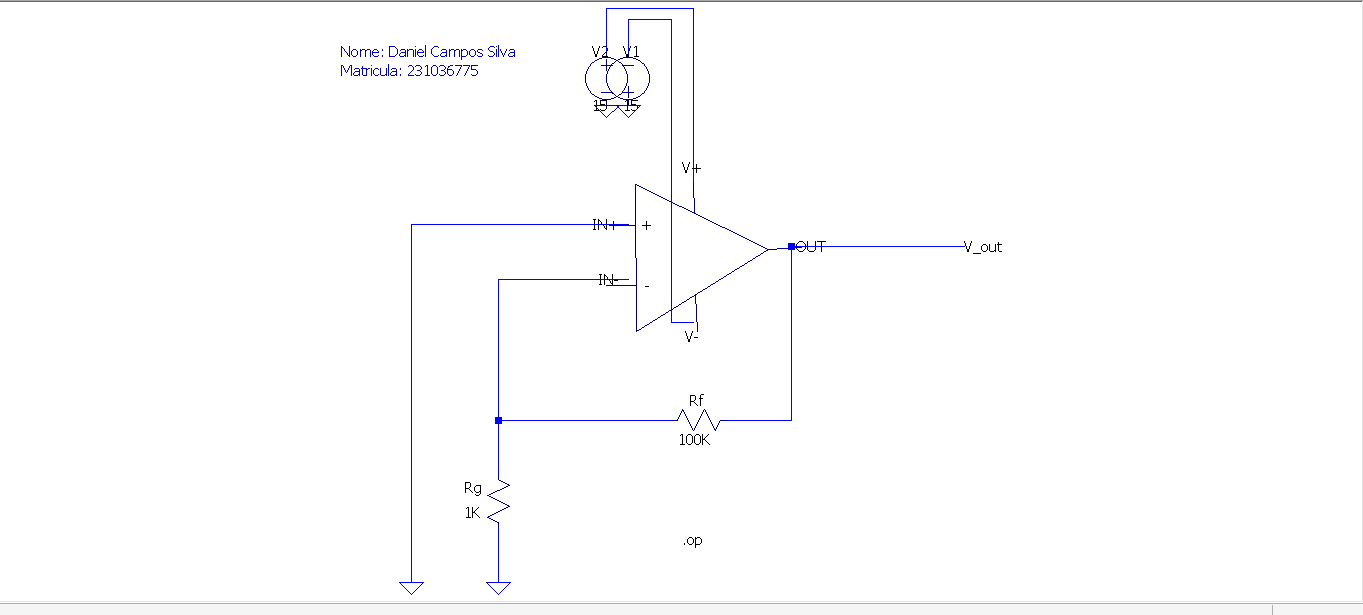
\includegraphics[width=\linewidth]{imgs/daniel/daniel_simulacao/item_1_tensão_offset.png}
    \vspace{2pt}
    {\small (a) Tensão de Offset}
\end{minipage}\hfill
\begin{minipage}{0.48\linewidth}
    \centering
    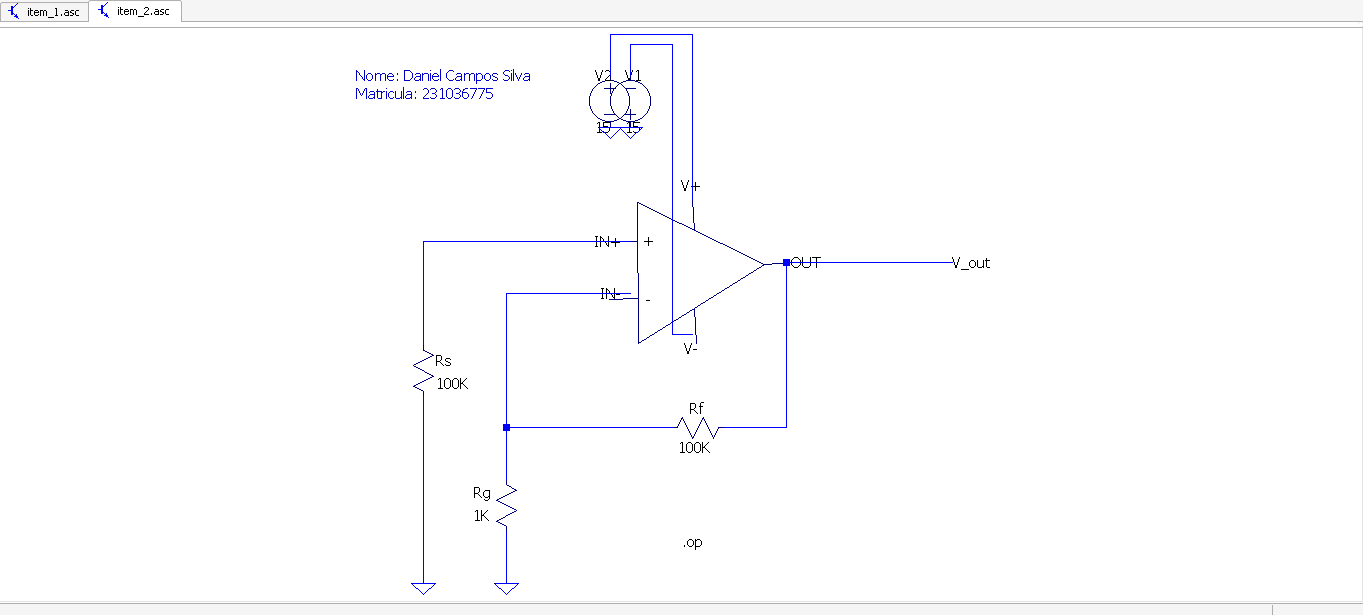
\includegraphics[width=\linewidth]{imgs/daniel/daniel_simulacao/item_2_corrente_de_polarização_LM741.png}
    \vspace{2pt}
    {\small (b) Corrente de Polarização (LM741)}
\end{minipage}

\vspace{12pt}

\begin{minipage}{0.48\linewidth}
    \centering
    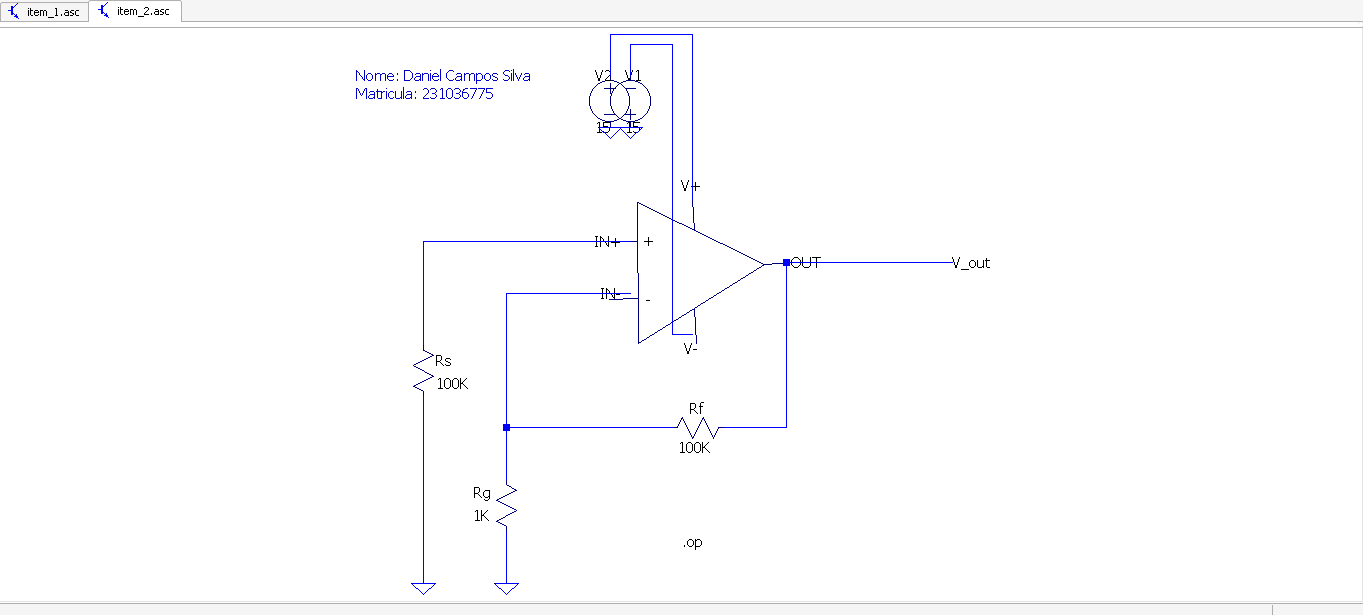
\includegraphics[width=\linewidth]{imgs/daniel/daniel_simulacao/item_5_corrente_de_polarização_TL064.png}
    \vspace{2pt}
    {\small (c) Corrente de Polarização (TL064)}
\end{minipage}\hfill
\begin{minipage}{0.48\linewidth}
    \centering
    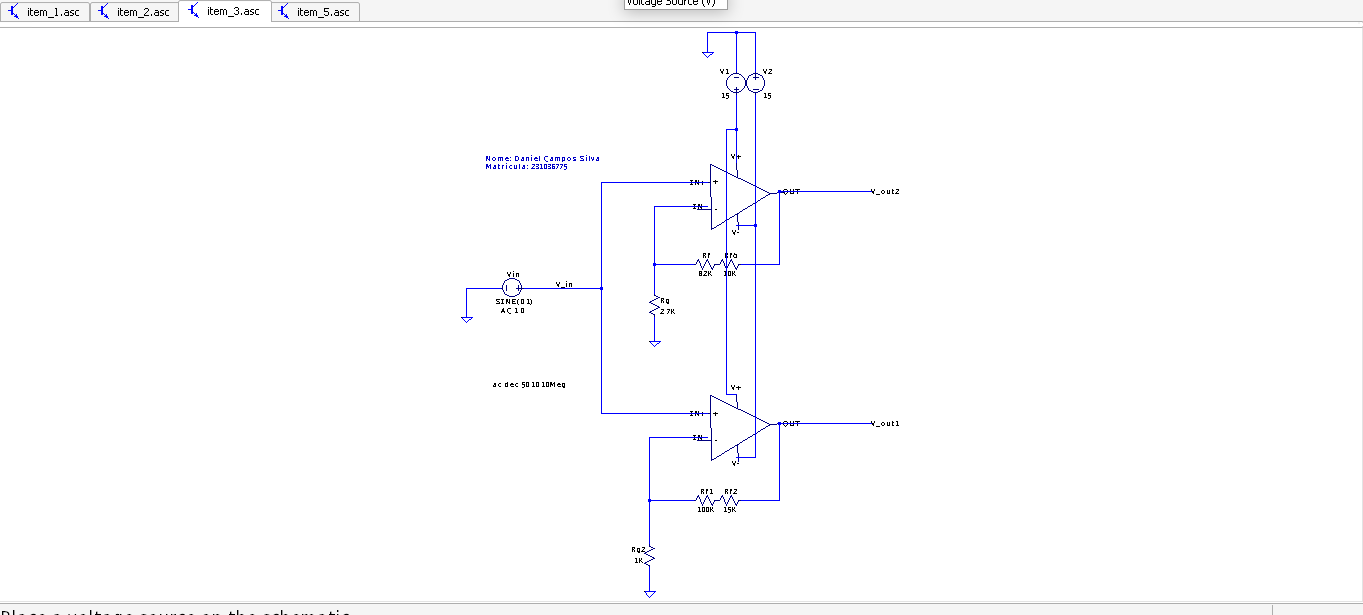
\includegraphics[width=\linewidth]{imgs/daniel/daniel_simulacao/item_3_resposta_em_frequência.png}
    \vspace{2pt}
    {\small (d) Resposta em Frequência}
\end{minipage}

\vspace{12pt}

\begin{minipage}{0.48\linewidth}
    \centering
    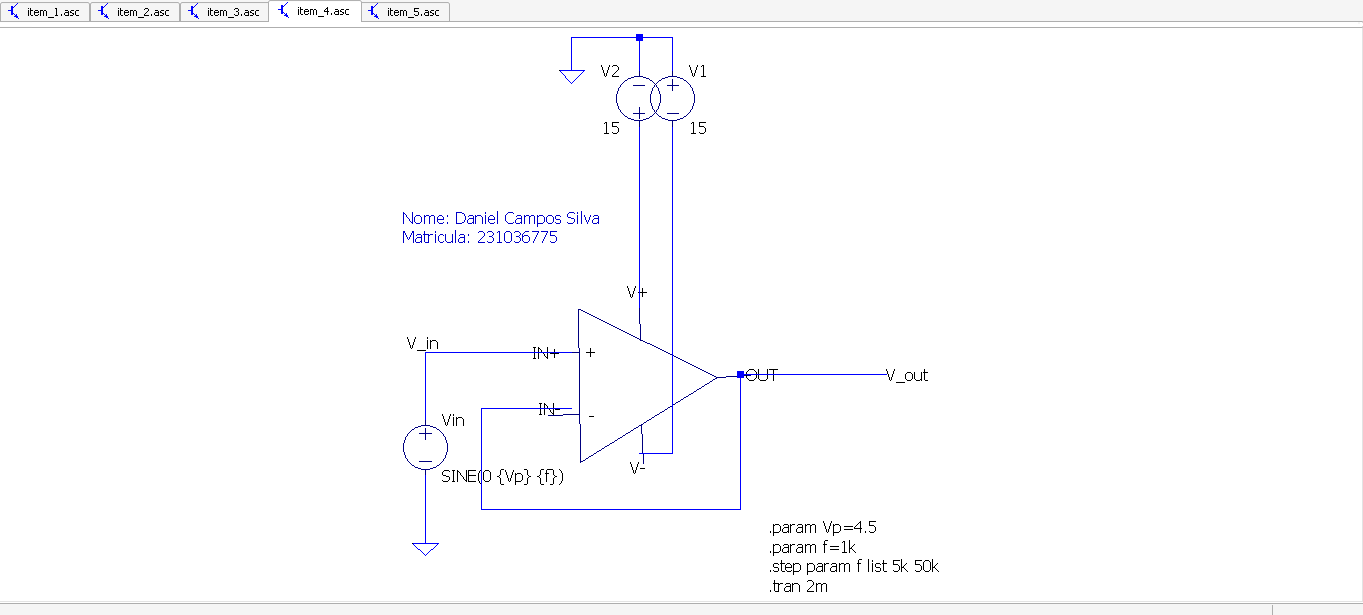
\includegraphics[width=\linewidth]{imgs/daniel/daniel_simulacao/item_4_slew_rate_LM741.png}
    \vspace{2pt}
    {\small (e) Slew Rate (LM741)}
\end{minipage}\hfill
\begin{minipage}{0.48\linewidth}
    \centering
    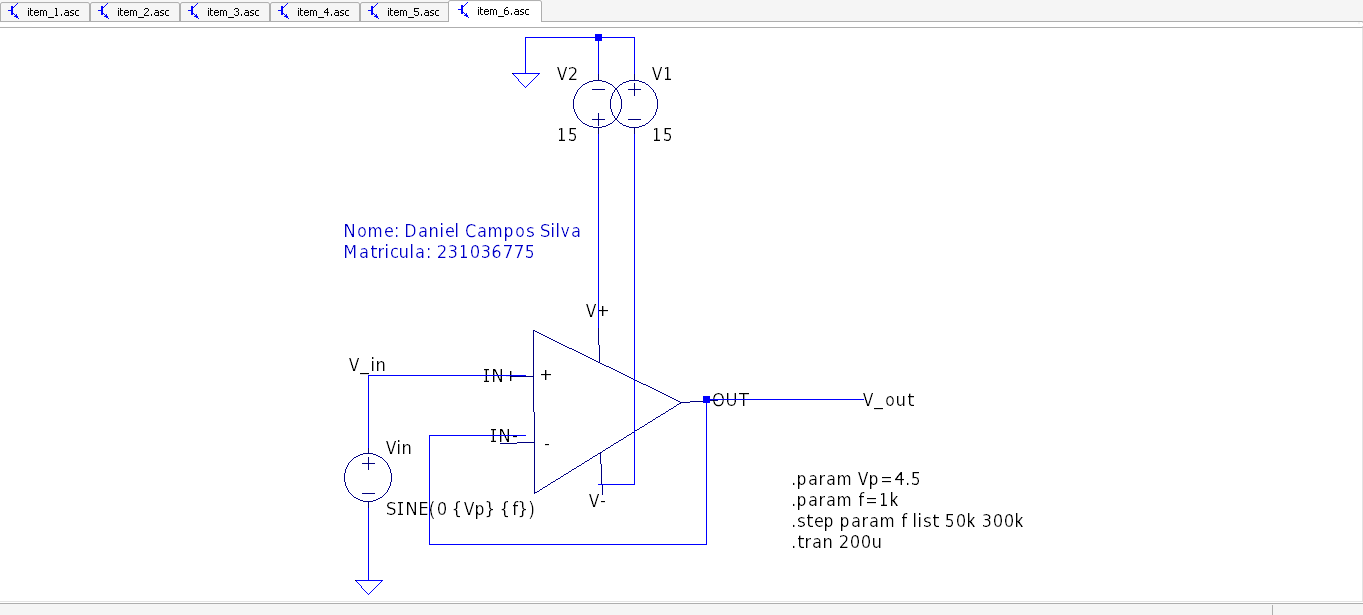
\includegraphics[width=\linewidth]{imgs/daniel/daniel_simulacao/item_6_slew_rate_TL064.png}
    \vspace{2pt}
    {\small (f) Slew Rate (TL064)}
\end{minipage}

\caption{Esquemáticos projetados para a matrícula 23/1036775, contendo os resistores E12 dimensionados e as diretivas de simulação aplicadas.}
\label{fig:circs_daniel}
\end{figure}

\subsubsection{Lurian Lima (22/2005395)}

\textbf{Configuração e Simulação dos Circuitos}

O roteiro determina $G_1=20+(5\bmod 21)=25$, $G_2=80+(39\bmod 41)=119$ e $V_p=2+\tfrac{5}{2}=4{,}5\text{ V}$. Os seis circuitos foram desenhados e simulados no LTspice com os símbolos do LM741 e do TL064 construídos no Roteiro 2, a partir da biblioteca \texttt{ene0046.lib}, e alimentação simétrica de $\pm15\text{ V}$, conforme a Figura~\ref{fig:circs_luri}. Cada esquemático traz uma única diretiva de análise ativa, configurada da seguinte forma:

\begin{itemize}
    \item \textbf{Tensão de Offset (Fig.~\ref{fig:circs_luri}a):} Amplificador não inversor de ganho 101, com $R_f=100\text{ k}\Omega$ e $R_g=1\text{ k}\Omega$, e a entrada não inversora ligada diretamente ao terra. A análise de ponto de operação (\texttt{.op}) fornece a tensão contínua na saída $v_o$, da qual se obtém $V_{os}=V_o/101$.

    \item \textbf{Corrente de Polarização (Fig.~\ref{fig:circs_luri}b e \ref{fig:circs_luri}c):} O circuito anterior foi alterado com a inclusão de $R_s=100\text{ k}\Omega$ entre o terra e a entrada não inversora (nó \texttt{ninv}). A análise \texttt{.op} foi feita em dois esquemáticos, um com o LM741 e outro com o TL064 no lugar dele. A diferença entre a saída com $R_s$ e a saída sem $R_s$ permite obter $I_b=\Delta V_o/(101\,R_s)$.

    \item \textbf{Resposta em Frequência (Fig.~\ref{fig:circs_luri}d):} Dois amplificadores não inversores com LM741 no mesmo arquivo, alimentados pela mesma fonte de sinal (\texttt{AC 1}, nó \texttt{vin}). Para o ganho baixo $G_1=25$, adotou-se $R_g=1\text{ k}\Omega$ e $R_f$ formado pela associação em série de dois resistores de $12\text{ k}\Omega$, totalizando $24\text{ k}\Omega$, o que dá $G_{1,\text{real}}=1+24/1=25$. Para o ganho alto $G_2=119$, adotou-se $R_g=1\text{ k}\Omega$ e $R_f$ formado por $100\text{ k}\Omega$ em série com $18\text{ k}\Omega$, totalizando $118\text{ k}\Omega$, o que dá $G_{2,\text{real}}=1+118/1=119$. Em ambos os casos, o ganho realizado coincide com o especificado. A análise \texttt{.ac dec 50 10 10Meg} faz uma varredura decádica de 10 Hz a 10 MHz com 50 pontos por década, faixa que cobre as duas frequências de corte esperadas, que ficam em torno de $f_T/G$.

    \item \textbf{Slew Rate (Fig.~\ref{fig:circs_luri}e e \ref{fig:circs_luri}f):} Seguidor de tensão alimentado por uma fonte senoidal \texttt{SINE(0 4.5 \{freq\})}, com a amplitude $V_p=4{,}5\text{ V}$ da matrícula. A análise de transiente \texttt{.tran 0 \{10/freq\} 0 \{1/(500*freq)\}} simula dez períodos de cada frequência, com passo máximo de $1/(500f)$, isto é, 500 pontos por período, o que resolve bem a inclinação da rampa na passagem por zero. A frequência é varrida por \texttt{.step param freq list}. No LM741 adotou-se $5\text{ kHz}$ e $50\text{ kHz}$: com o slew rate típico de $0{,}5\text{ V}/\mu\text{s}$ do datasheet, a senoide de $4{,}5\text{ V}$ passa a exigir mais do que o amplificador entrega a partir de $f=\mathrm{SR}/(2\pi V_p)\approx17{,}7\text{ kHz}$, de modo que a primeira frequência é acompanhada pela saída e a segunda já resulta em triângulo. Como o TL064 é mais rápido, as frequências foram escolhidas de novo, em $30\text{ kHz}$ e $400\text{ kHz}$, uma vez que as do LM741 não servem para evidenciar o limite dessa peça.
\end{itemize}

\begin{figure}[H]
\centering
\begin{minipage}{0.48\linewidth}
    \centering
    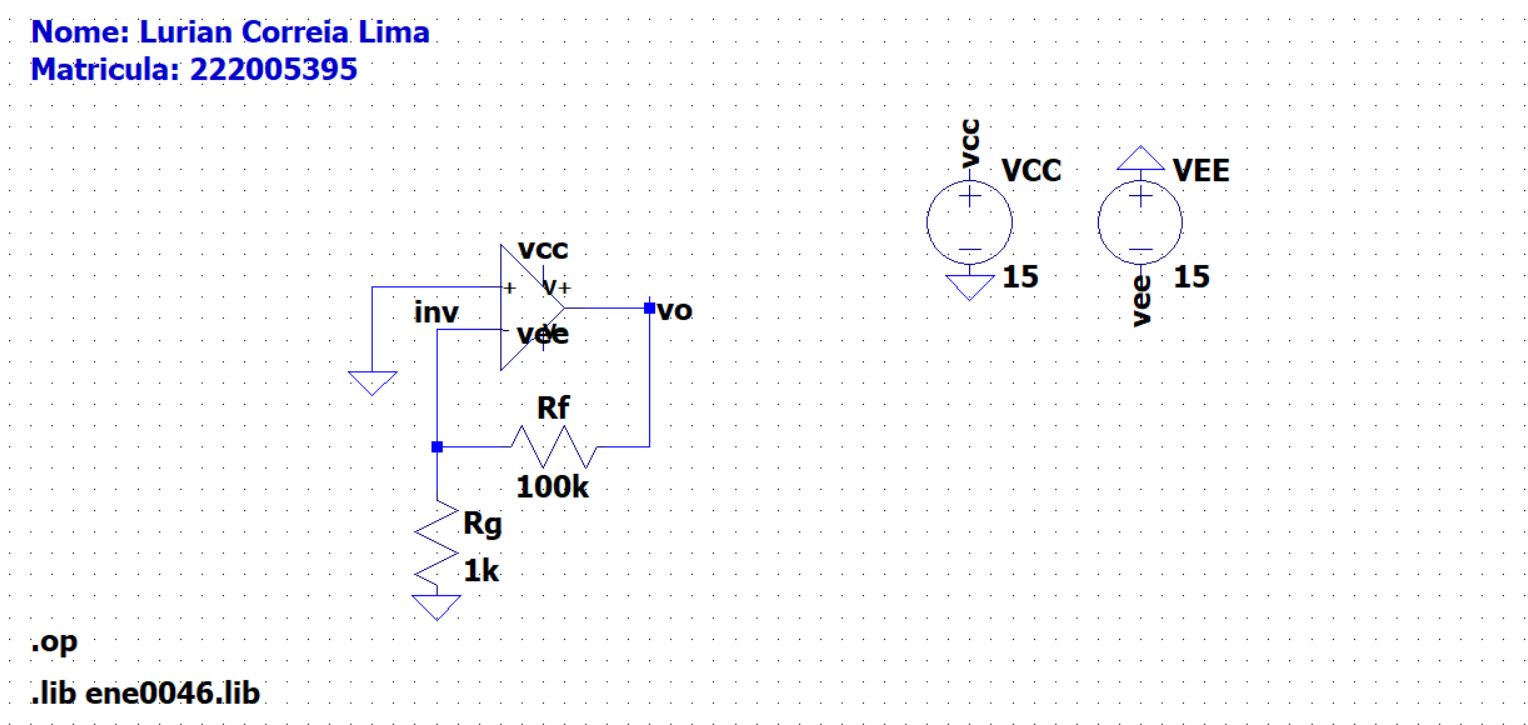
\includegraphics[width=\linewidth]{imgs/luri/simulacao/Item 1 - Tensao de offset do LM741.png}
    \vspace{2pt}
    {\small (a) Tensão de Offset}
\end{minipage}\hfill
\begin{minipage}{0.48\linewidth}
    \centering
    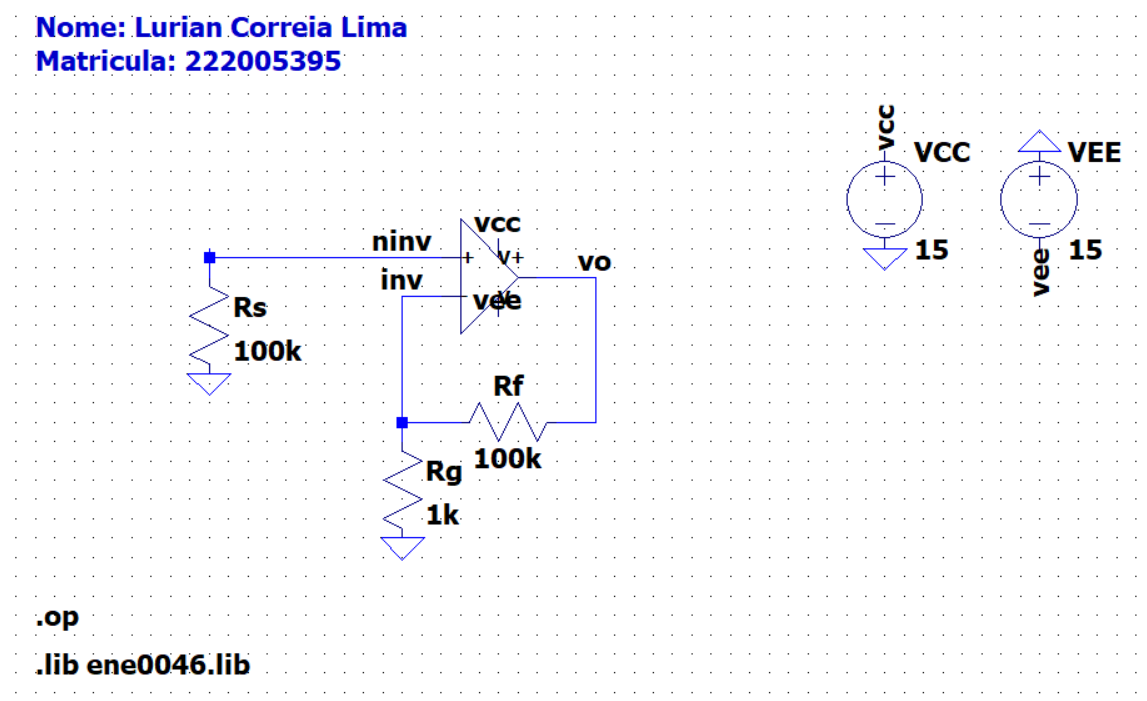
\includegraphics[width=\linewidth]{imgs/luri/simulacao/Item 2 - Corrente de polarizacao do LM741.png}
    \vspace{2pt}
    {\small (b) Corrente de Polarização (LM741)}
\end{minipage}

\vspace{12pt}

\begin{minipage}{0.48\linewidth}
    \centering
    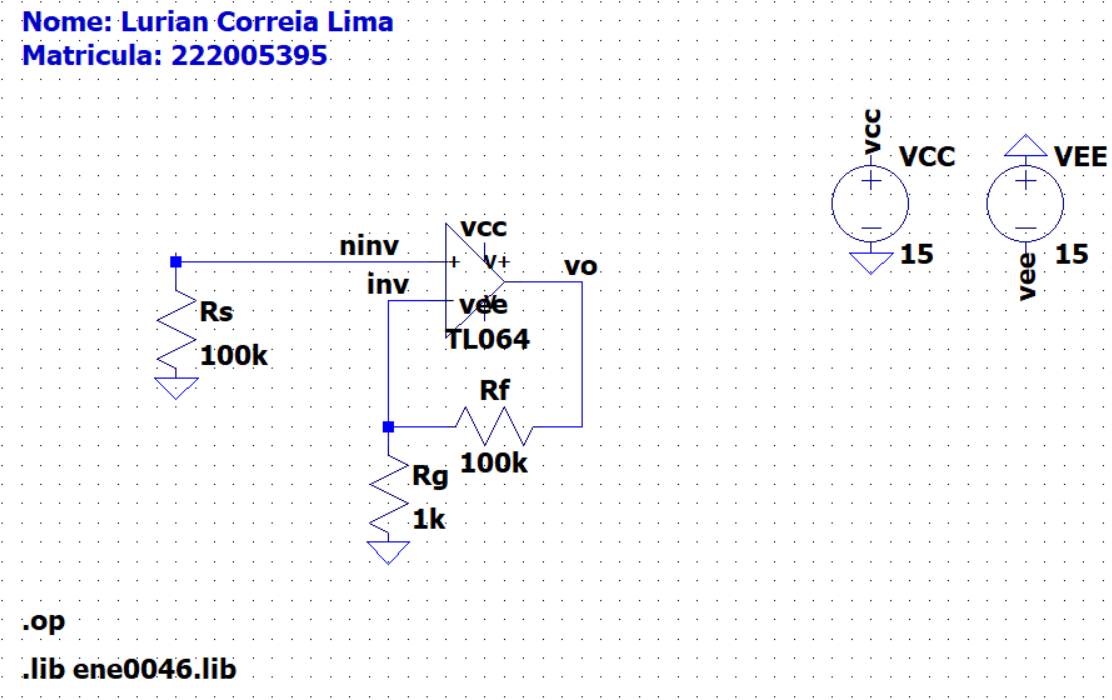
\includegraphics[width=\linewidth]{imgs/luri/simulacao/Item 5 - Corrente de polarizacao do TL064.png}
    \vspace{2pt}
    {\small (c) Corrente de Polarização (TL064)}
\end{minipage}\hfill
\begin{minipage}{0.48\linewidth}
    \centering
    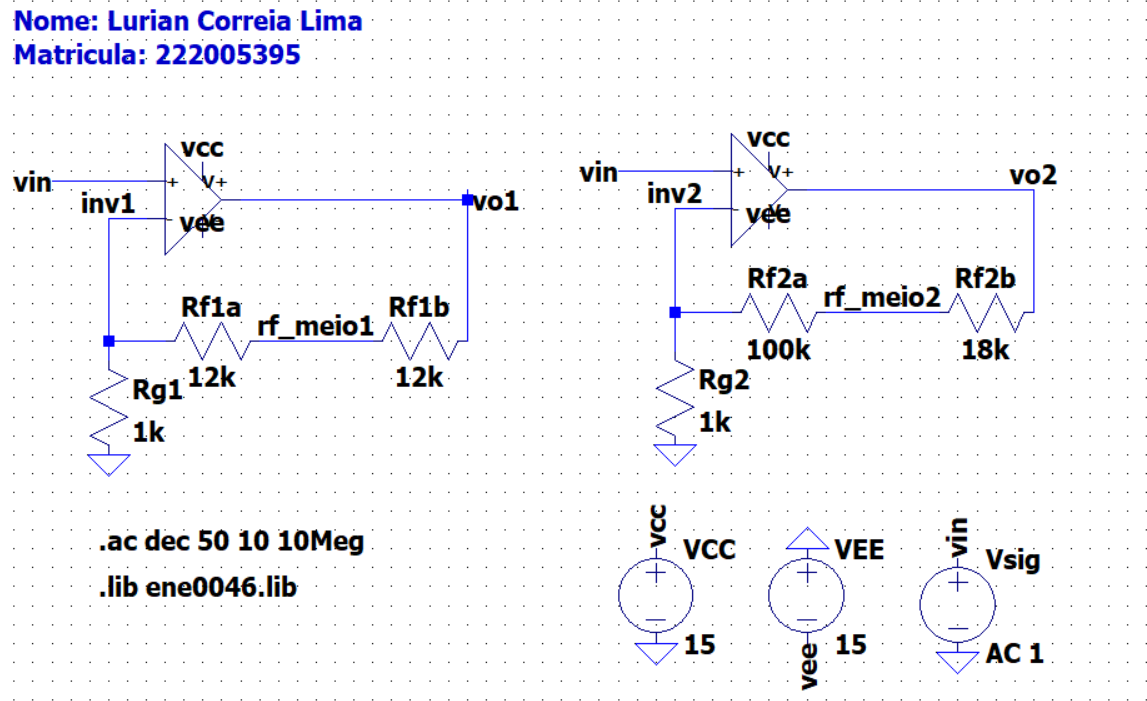
\includegraphics[width=\linewidth]{imgs/luri/simulacao/Item 3 - Resposta em frequencia do LM741.png}
    \vspace{2pt}
    {\small (d) Resposta em Frequência}
\end{minipage}

\vspace{12pt}

\begin{minipage}{0.48\linewidth}
    \centering
    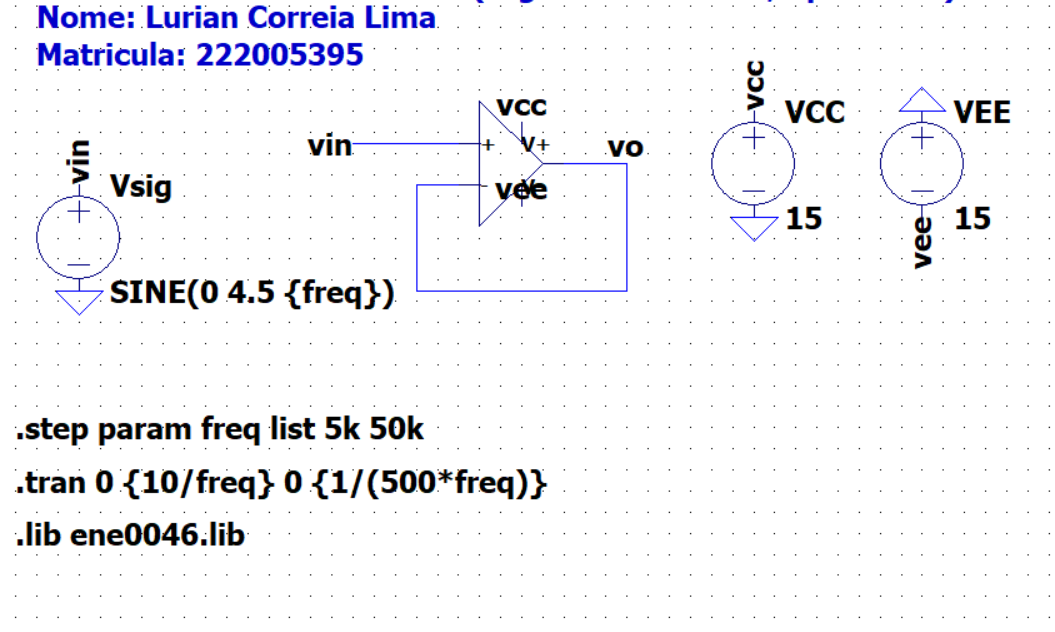
\includegraphics[width=\linewidth]{imgs/luri/simulacao/Item 4 - Slew rate do LM741.png}
    \vspace{2pt}
    {\small (e) Slew Rate (LM741)}
\end{minipage}\hfill
\begin{minipage}{0.48\linewidth}
    \centering
    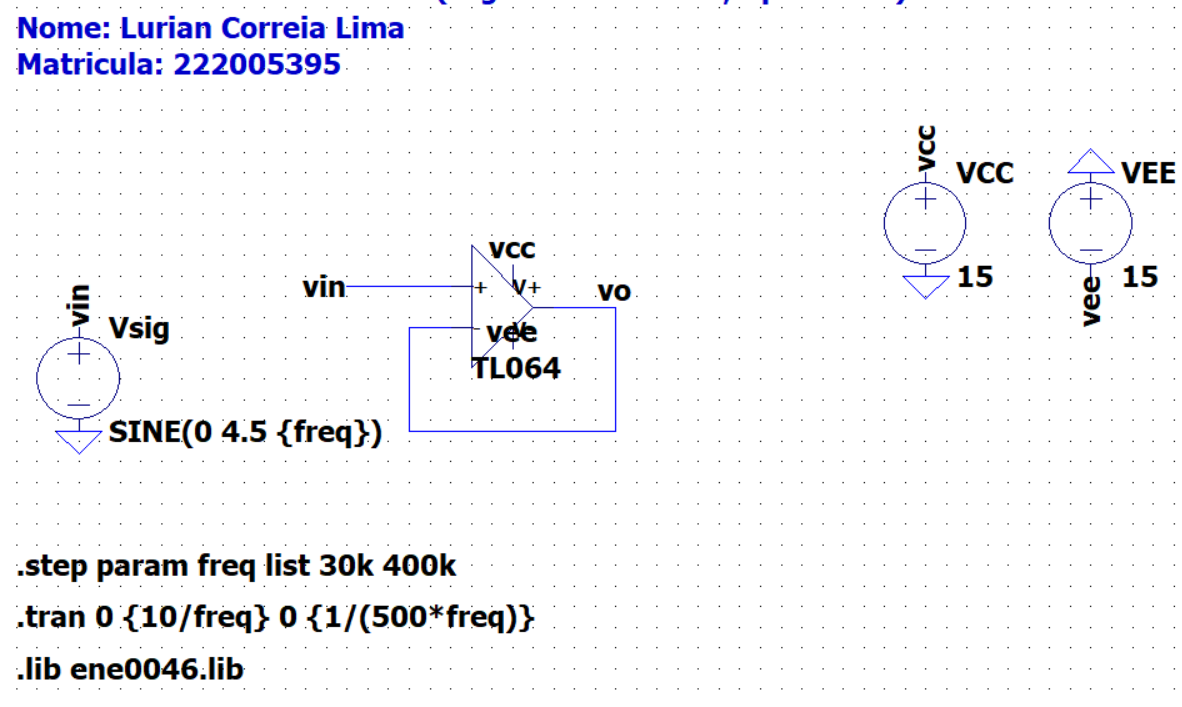
\includegraphics[width=\linewidth]{imgs/luri/simulacao/Item 6 - Slew rate do TL064.png}
    \vspace{2pt}
    {\small (f) Slew Rate (TL064)}
\end{minipage}

\caption{Esquemáticos projetados para a matrícula 22/2005395, contendo os resistores E12 dimensionados e as diretivas de simulação aplicadas.}
\label{fig:circs_luri}
\end{figure}

\subsection{Montagem em bancada}

A montagem em bancada foi realizada de acordo com a especificação da Equipe 2, que estabelece ganho baixo $G_1=13$, amplitude de pico $V_p=2{,}5$~V para o ensaio de \textit{slew rate} e ganho alto igual a 101. Os amplificadores operacionais foram alimentados com tensão simétrica de $\pm15$~V, utilizando capacitores de desacoplamento de 100~nF entre as alimentações e o terra, conforme especificado no roteiro.

Antes da montagem dos circuitos, os resistores utilizados foram medidos individualmente. Os valores obtidos foram utilizados posteriormente na simulação da montagem.

\begin{table}[H]
\centering
\caption{Valores dos resistores medidos antes da montagem.}
\label{tab:resistores_bancada}
\begin{tabular}{c c c}
\hline
\textbf{Componente} & \textbf{Valor nominal} & \textbf{Valor medido} \\
\hline
$R_f$ & $100~\mathrm{k}\Omega$ & $101~\mathrm{k}\Omega$ \\
$R_g$ & $1~\mathrm{k}\Omega$ & $983~\Omega$ \\
$R_f'$ & $10~\mathrm{k}\Omega$ & $9{,}816~\mathrm{k}\Omega$ \\
$R_g'$ & $820~\Omega$ & $807~\Omega$ \\
$R_s$ & $100~\mathrm{k}\Omega$ & $98{,}770~\mathrm{k}\Omega$ \\
\hline
\end{tabular}
\end{table}

\subsubsection{Tensão de offset}

Inicialmente, foi montado o amplificador não inversor com ganho nominal 101 (Figuras~\ref{fig:montagem_offset_lm741} e~\ref{fig:montagem_offset_tl064}), utilizando $R_f=100~\mathrm{k}\Omega$ e $R_g=1~\mathrm{k}\Omega$. A entrada não inversora foi conectada diretamente ao terra, de modo que qualquer tensão contínua observada na saída estivesse associada principalmente à tensão de offset do amplificador operacional.

Para o LM741, foi medida uma tensão contínua de saída de $169$~mV. Considerando o ganho de 101 utilizado no ensaio, a tensão de offset correspondente é

$$
V_{OS}=\frac{V_O}{101}
=\frac{169~\mathrm{mV}}{101}
\approx1{,}67~\mathrm{mV}.
$$

Na sequência, o LM741 foi substituído pelo TL064, mantendo-se a mesma configuração de ensaio. Para o TL064, foi medida uma tensão de saída de $-49{,}5$~mV, resultando em

$$
V_{OS}=\frac{-49{,}5~\mathrm{mV}}{101}
\approx-0{,}490~\mathrm{mV}.
$$

\begin{table}[H]
\centering
\caption{Tensão de offset medida para os amplificadores operacionais.}
\label{tab:offset_bancada}
\begin{tabular}{c c c}
\hline
\textbf{Amplificador} & \textbf{$V_O$ medido} & \textbf{$V_{OS}=V_O/101$} \\
\hline
LM741 & $169$~mV & $1{,}67$~mV \\
TL064 & $-49{,}5$~mV & $-0{,}490$~mV \\
\hline
\end{tabular}
\end{table}

\begin{figure}[H]
\centering
% Inserir aqui a fotografia da montagem utilizada no ensaio de tensão de offset.
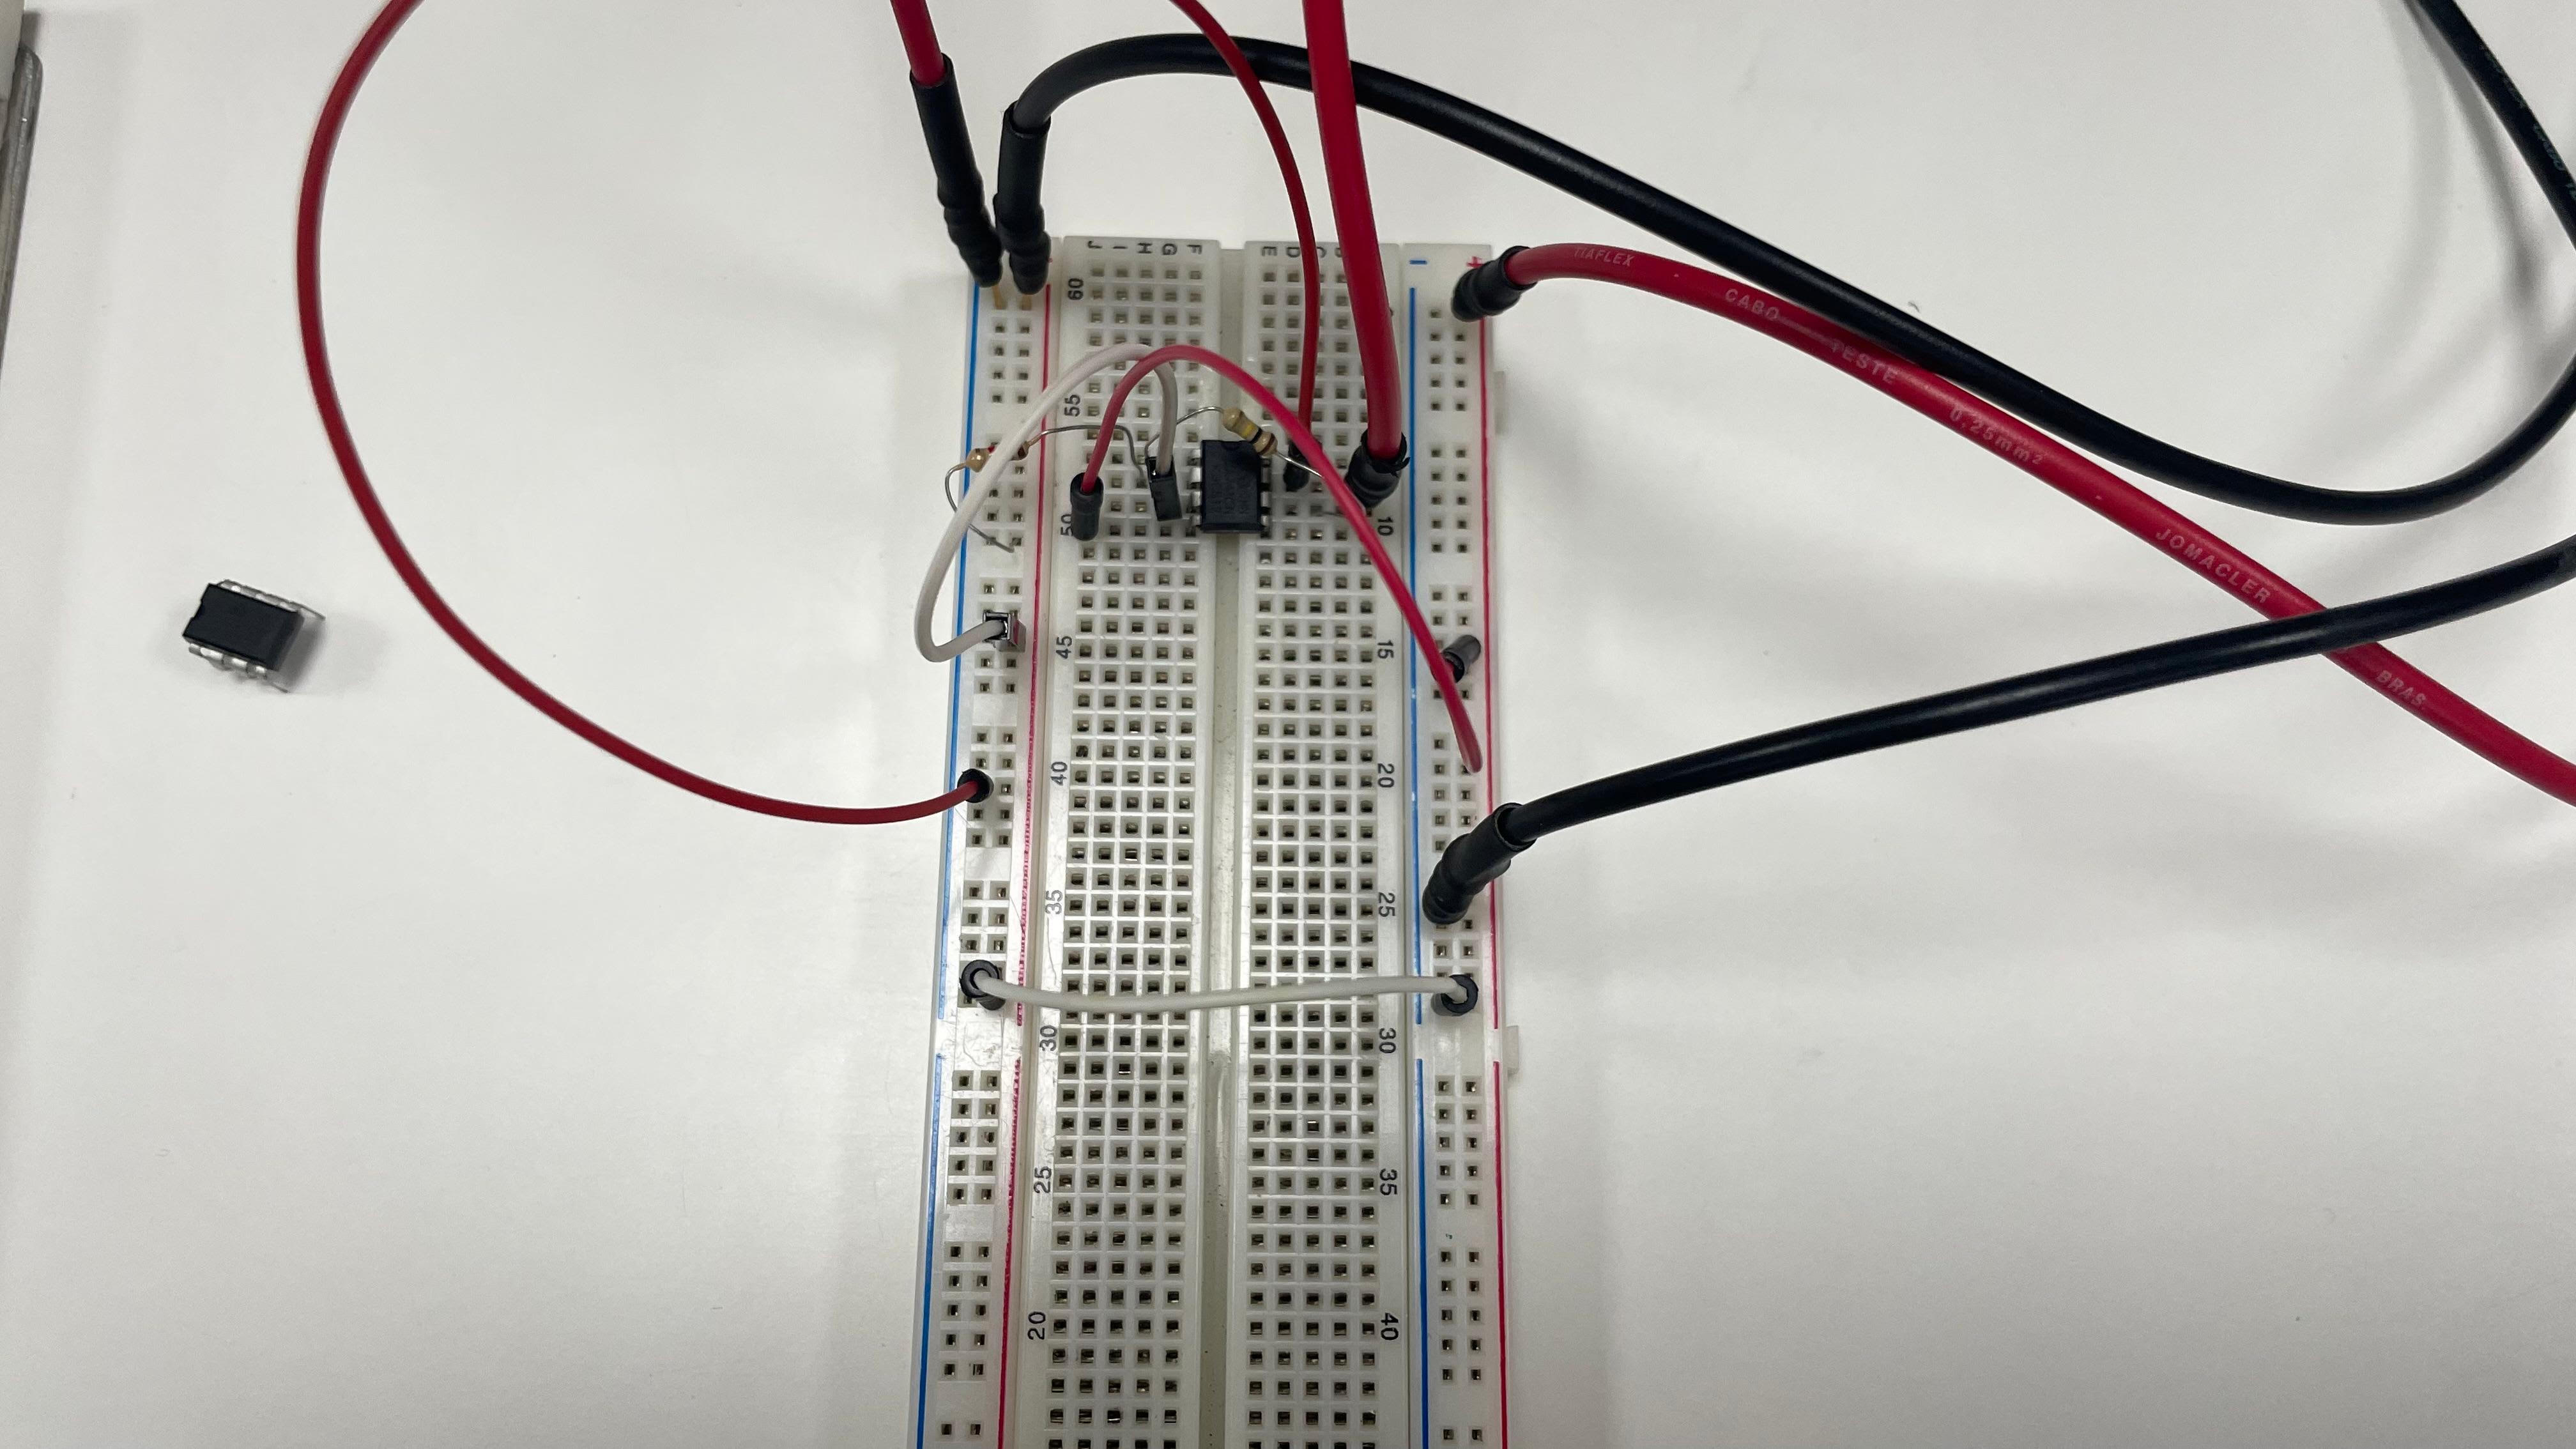
\includegraphics[width=0.65\textwidth]{imgs/montagem/3.3tensaooffset.jpg}
\caption{LM741: Montagem em bancada utilizada para a medição da tensão de offset.}
\label{fig:montagem_offset_lm741}
\end{figure}

\begin{figure}[H]
\centering
% Inserir aqui a fotografia da montagem utilizada no ensaio de tensão de offset.
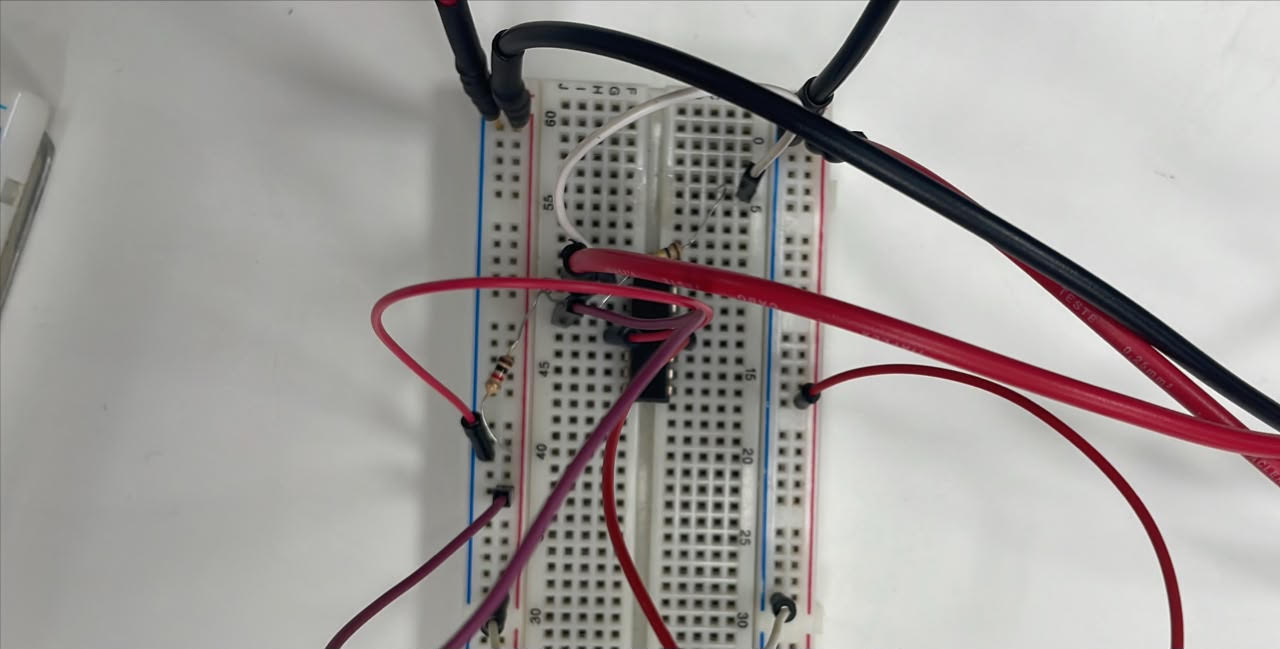
\includegraphics[width=0.65\textwidth]{imgs/montagem/3.3tensaooffset2.jpg}
\caption{TL064: Montagem em bancada utilizada para a medição da tensão de offset.}
\label{fig:montagem_offset_tl064}
\end{figure}

\subsubsection{Corrente de polarização}

Para a medição da corrente de polarização, o fio que conectava a entrada não inversora ao terra foi substituído pelo resistor $R_s=98{,}770~\mathrm{k}\Omega$ (Figuras~\ref{fig:montagem_polarizacao_lm741} e~\ref{fig:montagem_polarizacao_tl064}). A tensão de saída foi então medida novamente, permitindo determinar a variação de tensão causada pela corrente de polarização.

Para o LM741, a tensão de saída passou de $169$~mV, obtida no ensaio de offset, para $2{,}7$~mV. Assim,

$$
\Delta V_O=2{,}7-169=-166{,}3~\mathrm{mV}.
$$

A corrente de polarização resulta em

$$
I_B=
\frac{\Delta V_O}{101R_s}
=
\frac{-166{,}3~\mathrm{mV}}
{101\cdot98{,}770~\mathrm{k}\Omega}
\approx-16{,}7~\mathrm{nA}.
$$

A redução da tensão de saída indica que, nesse ensaio, a corrente de polarização do LM741 possui sentido compatível com uma corrente entrando pela entrada do amplificador operacional.

Para o TL064, a tensão de saída passou de $-49{,}5$~mV para $32{,}598$~mV. Portanto,

$$
\Delta V_O=32{,}598-(-49{,}5)
=82{,}098~\mathrm{mV},
$$

e

$$
I_B=
\frac{82{,}098~\mathrm{mV}}
{101\cdot98{,}770~\mathrm{k}\Omega}
\approx8{,}23~\mathrm{nA}.
$$

Nesse caso, o aumento da tensão de saída indica um sentido de corrente de polarização oposto ao observado no ensaio com o LM741.

\begin{table}[H]
\centering
\caption{Medição da corrente de polarização dos amplificadores operacionais.}
\label{tab:polarizacao_bancada}
\begin{tabular}{c c c c}
\hline
\textbf{Amplificador} & \textbf{$V_O$ com $R_s$} & \textbf{$\Delta V_O$} & \textbf{$I_B$} \\
\hline
LM741 & $2{,}7$~mV & $-166{,}3$~mV & $-16{,}7$~nA \\
TL064 & $32{,}598$~mV & $82{,}098$~mV & $8{,}23$~nA \\
\hline
\end{tabular}
\end{table}

A diferença entre os degraus observados para o LM741 e o TL064 está associada às características distintas dos estágios de entrada dos dois amplificadores operacionais. O LM741 possui entrada bipolar, enquanto o TL064 utiliza entrada JFET, resultando em correntes de polarização de ordens de grandeza e sentidos diferentes.

\begin{figure}[H]
\centering
% Inserir aqui a fotografia da montagem com o resistor Rs.
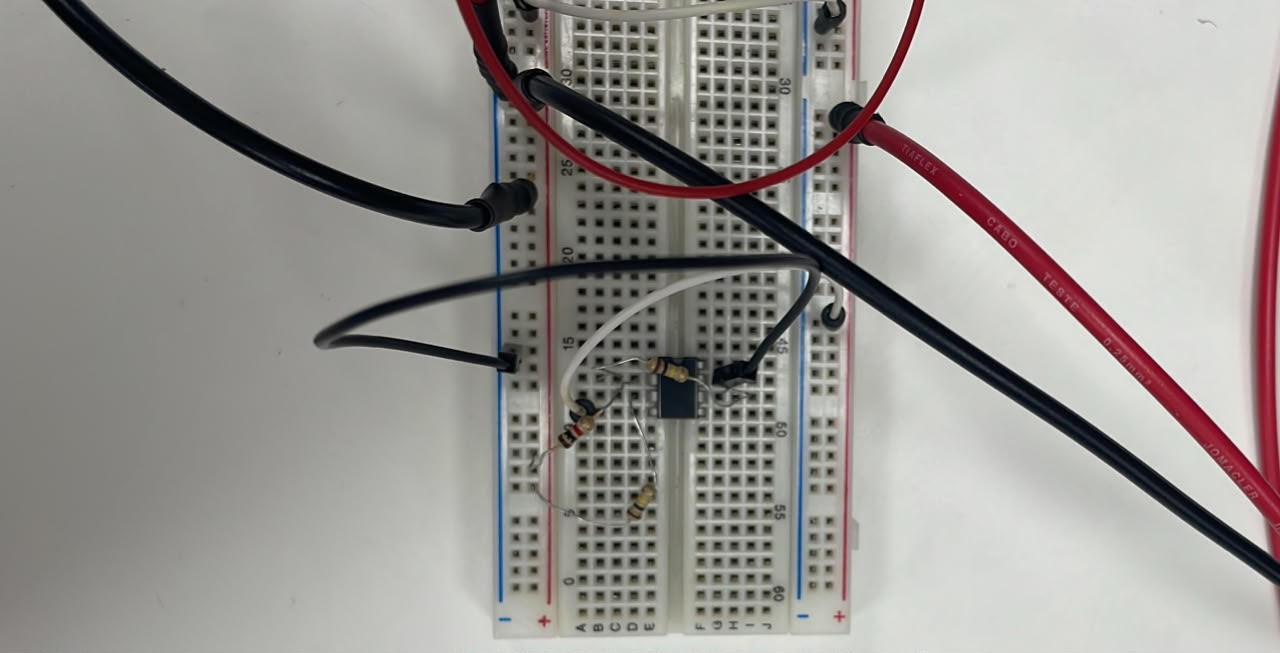
\includegraphics[width=0.65\textwidth]{imgs/montagem/3.4LM741.jpg}
\caption{LM741: Montagem utilizada para a medição da corrente de polarização.}
\label{fig:montagem_polarizacao_lm741}
\end{figure}

\begin{figure}[H]
\centering
% Inserir aqui a fotografia da montagem com o resistor Rs.
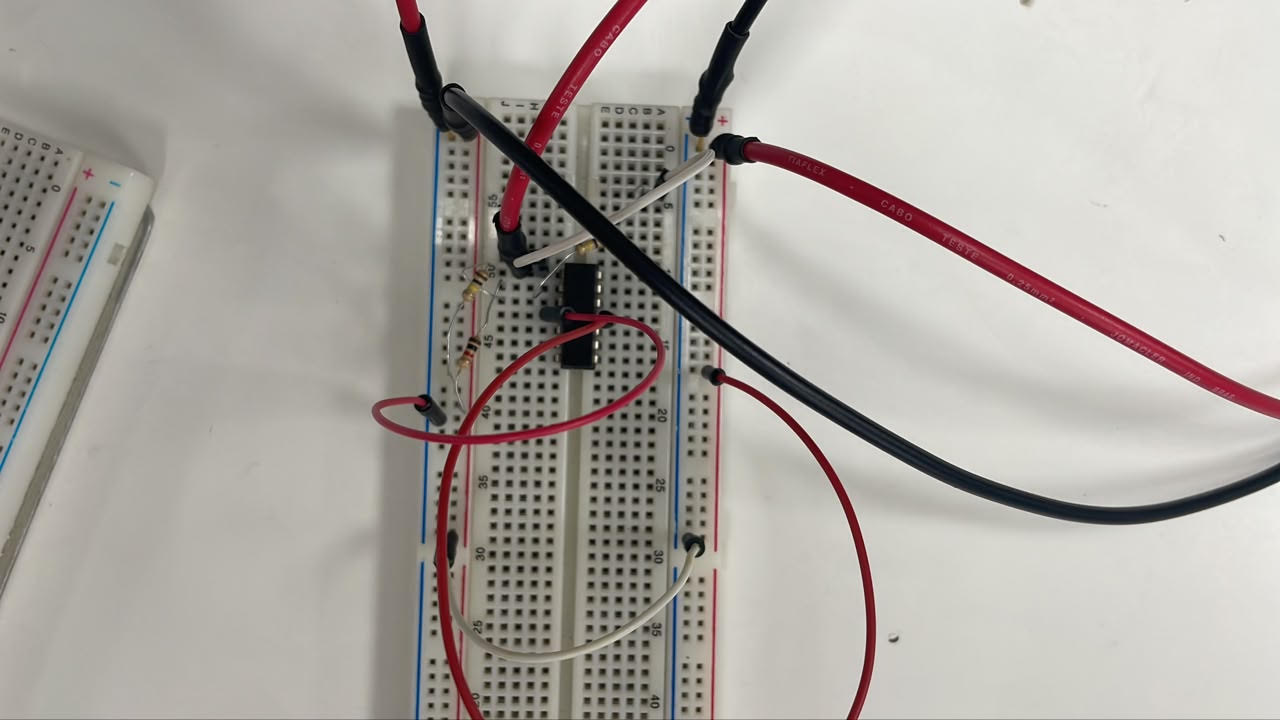
\includegraphics[width=0.65\textwidth]{imgs/montagem/3.4TL064.jpg}
\caption{TL064: Montagem utilizada para a medição da corrente de polarização.}
\label{fig:montagem_polarizacao_tl064}
\end{figure}

\subsubsection{Resposta em frequência}

Para a análise da resposta em frequência, foi utilizado o amplificador não inversor de ganho baixo da Equipe 2. Os resistores escolhidos foram $R_f'=10~\mathrm{k}\Omega$ e $R_g'=820~\Omega$, cujos valores medidos foram, respectivamente, $9{,}816~\mathrm{k}\Omega$ e $807~\Omega$.

O ganho efetivamente realizado pela razão entre os valores medidos é

$$
G_1=
1+\frac{R_f'}{R_g'}
=
1+\frac{9{,}816}{0{,}807}
\approx13{,}17.
$$

Também foi analisado o estágio de ganho alto, utilizando os valores medidos $R_f=101~\mathrm{k}\Omega$ e $R_g=983~\Omega$. Com esses valores, o ganho resistivo correspondente é

$$
G_{101,\mathrm{med}}=
1+\frac{101}{0{,}983}
\approx103{,}75.
$$

A resposta em frequência foi obtida mantendo a amplitude de entrada constante e aumentando progressivamente a frequência do sinal. A montagem está na Figura~\ref{fig:resposta_frequencia}, e os valores medidos são apresentados nas Tabelas~\ref{tab:freq_g1_equipe} e~\ref{tab:freq_g2_equipe} da Seção~5.2.




\begin{figure}[H]
\centering
% Inserir aqui o gráfico de ganho em função da frequência, com eixo de frequência logarítmico.
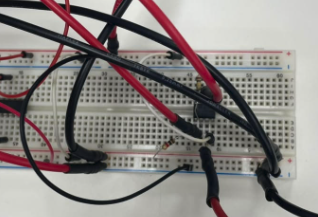
\includegraphics[width=0.85\textwidth]{imgs/montagem/3.5montagem.png}
\caption{Montagem do circuito de resposta em frequência.}
\label{fig:resposta_frequencia}
\end{figure}

A frequência de corte de cada estágio e o respectivo produto ganho-banda serão determinados a partir das curvas experimentais, considerando a frequência na qual o ganho cai para aproximadamente $0{,}707$ do valor de referência.

\subsubsection{Slew rate}

O ensaio de \textit{slew rate} foi realizado configurando o amplificador operacional como seguidor de tensão. Para a Equipe 2, a senoide aplicada possui amplitude de pico $V_p=2{,}5$~V. A frequência foi aumentada progressivamente até que a saída deixasse de apresentar comportamento senoidal e passasse a apresentar formato aproximadamente triangular. A montagem está na Figura~\ref{fig:montagem_slew}.



A frequência limite pode ser relacionada ao \textit{slew rate} pela expressão

$$
SR=2\pi f V_p.
$$

Assim, após a determinação do \textit{slew rate} a partir da inclinação da rampa medida no osciloscópio, pode-se calcular a frequência teórica correspondente e compará-la com a frequência observada experimentalmente.



\begin{figure}[H]
\centering
% Inserir aqui a captura do osciloscópio para o TL064.
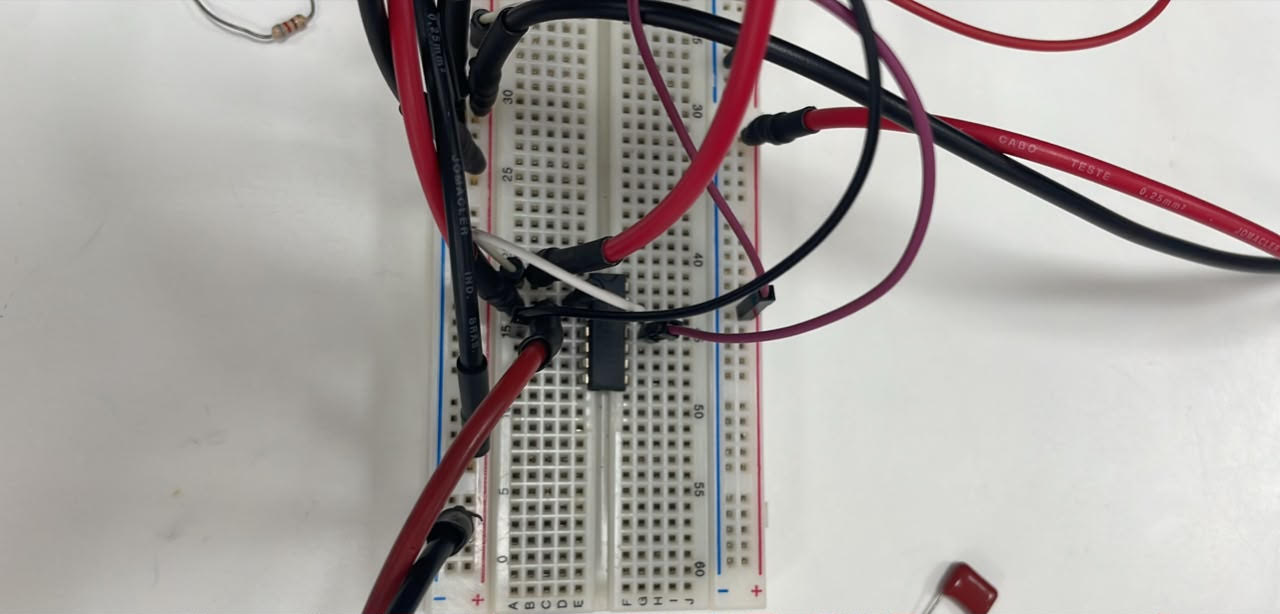
\includegraphics[width=0.75\textwidth]{imgs/montagem/3.6slewrate.jpg}
\caption{Montagem do circuito para o ensaio de \textit{slew rate}.}
\label{fig:montagem_slew}
\end{figure}


\subsection{Simulação da montagem}

Nesta etapa, os circuitos utilizados na bancada foram reconstruídos no LTspice utilizando os valores reais dos componentes medidos antes da montagem. Dessa forma, buscou-se reproduzir nas simulações as mesmas condições utilizadas experimentalmente, permitindo posteriormente confrontar os resultados de projeto, simulação e medição.

\begin{nota}{Três comparações, três causas diferentes}
Os resultados são confrontados em três pares, discutidos separadamente na Seção~6.

\smallskip
\textbf{Cálculo analítico contra simulação de projeto.} Verifica a álgebra e o esquemático de cada
integrante.

\smallskip
\textbf{Simulação de projeto contra simulação da montagem.} Mede o efeito da tolerância dos
resistores, isto é, da distância entre o valor nominal e o valor real das peças usadas.

\smallskip
\textbf{Simulação da montagem contra medição.} Verifica se o modelo descreve o circuito real.
Diferenças aqui apontam para o que o modelo não representa: a dispersão entre unidades do mesmo
CI, a fuga no protoboard ou os limites dos instrumentos.
\end{nota}

\subsubsection{Tensão de offset}

O circuito do amplificador não inversor de ganho 101 foi reconstruído utilizando os valores medidos de $R_f$ e $R_g$. A entrada não inversora foi conectada ao terra, reproduzindo a condição utilizada na bancada para a determinação da tensão de offset.

\begin{figure}[H]
\centering
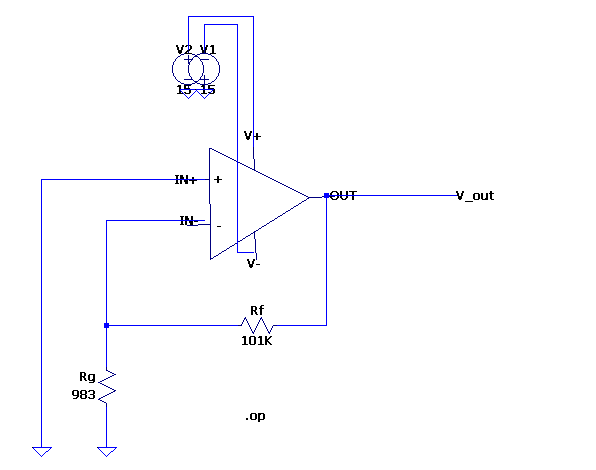
\includegraphics[width=0.75\textwidth]{imgs/simulacao/3.3circuitosimuladoLM741.png}
\caption{Simulação do circuito do LM741 utilizado para determinação da tensão de offset.}
\label{fig:sim_offset_lm741}
\end{figure}

\begin{figure}[H]
\centering
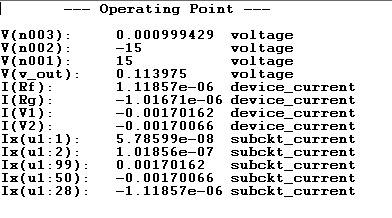
\includegraphics[width=0.75\textwidth]{imgs/simulacao/3.3resultadosimuladoLM741.png}
\caption{Resultados da simulação da tensão de offset para o LM741.}
\label{fig:sim_res_offset_lm741}
\end{figure}

O mesmo procedimento e análise foram realizados para o TL064:

\begin{figure}[H]
\centering
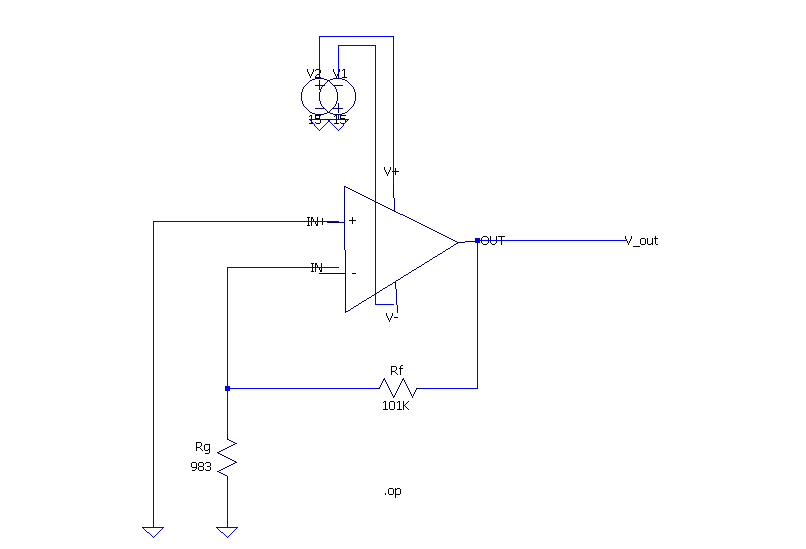
\includegraphics[width=0.75\textwidth]{imgs/simulacao/3.3circuitosimuladoTL064.png}
\caption{Simulação do circuito do TL064 utilizado para determinação da tensão de offset.}
\label{fig:sim_offset_tl064}
\end{figure}

\begin{figure}[H]
\centering
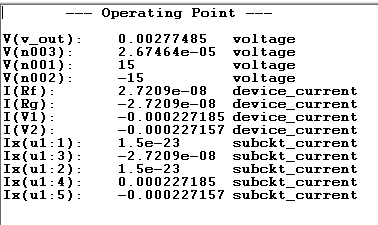
\includegraphics[width=0.75\textwidth]{imgs/simulacao/3.3resultadosimuladoTL064.png}
\caption{Resultados da simulação da tensão de offset para o TL064.}
\label{fig:sim_res_offset_tl064}
\end{figure}

Para o LM741 (Figuras~\ref{fig:sim_offset_lm741} e~\ref{fig:sim_res_offset_lm741}), a tensão de saída obtida na simulação foi de $0{,}113975~\mathrm{V}$, correspondendo a uma tensão de offset de

$$
V_{OS,\mathrm{sim}}=
\frac{V_{O,\mathrm{sim}}}{101}
=\frac{0{,}113975}{101}
\approx 1{,}13\times 10^{-3}~\mathrm{V}.
$$

Para o TL064 (Figuras~\ref{fig:sim_offset_tl064} e~\ref{fig:sim_res_offset_tl064}), a mesma divisão resulta em $V_{OS,\mathrm{sim}}\approx0{,}027$~mV. A divisão por 101 usa o ganho nominal; com o ganho dos resistores medidos, $103{,}75$, o offset do modelo do LM741 é $0{,}113975/103{,}75\approx1{,}10$~mV, como discutido na Seção~6.2.

\subsubsection{Corrente de polarização}

Para a simulação da corrente de polarização, o resistor $R_s=98{,}770~\mathrm{k}\Omega$ foi inserido entre a entrada não inversora e o terra. A diferença entre a tensão de saída dessa configuração e a tensão obtida no ensaio de offset permite determinar a corrente de polarização simulada.

\begin{figure}[H]
\centering
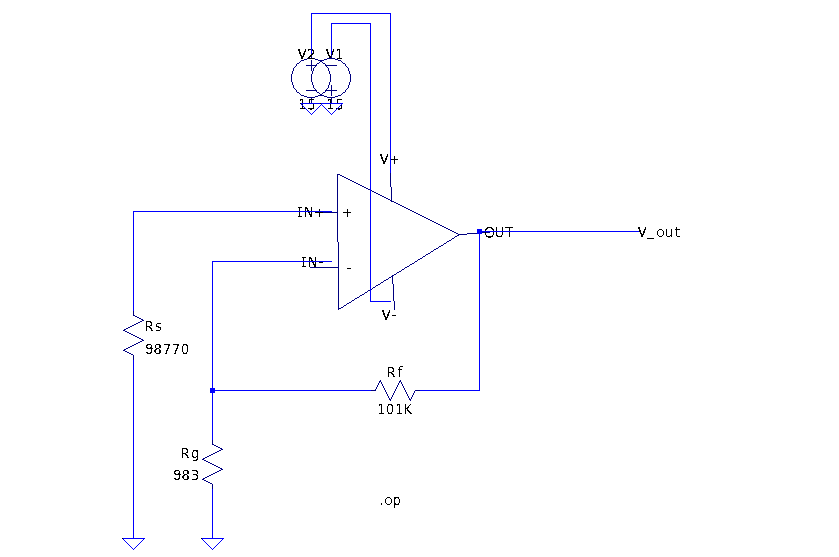
\includegraphics[width=0.75\textwidth]{imgs/simulacao/3.4circuitosimuladoLM741.png}
\caption{Simulação do circuito de corrente de polarização com o LM741.}
\label{fig:sim_polarizacao_lm741}
\end{figure}

\begin{figure}[H]
\centering
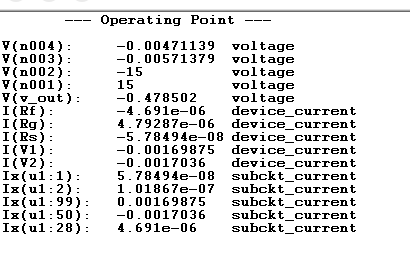
\includegraphics[width=0.75\textwidth]{imgs/simulacao/3.4resultadosimuladoLM741.png}
\caption{Resultados da simulação da corrente de polarização para o LM741.}
\label{fig:sim_res_polarizacao_lm741}
\end{figure}

Para o LM741,

$$
\Delta V_{O,\mathrm{sim}}=-0{,}592477~\mathrm{V}
$$

e

$$
I_{B,\mathrm{sim}}=
\frac{\Delta V_{O,\mathrm{sim}}}
{101R_s}
=\frac{-0{,}592477}
{101\cdot 98{,}770\times 10^3}
\approx -5{,}94\times 10^{-8}~\mathrm{A}.
$$

O mesmo procedimento foi realizado para o TL064 (Figuras~\ref{fig:sim_polarizacao_tl064} e~\ref{fig:sim_res_polarizacao_tl064}). O modelo não apresenta corrente de entrada mensurável: a corrente em $R_s$ é da ordem de $10^{-23}$~A e a saída varia apenas $\Delta V_{O,\mathrm{sim}}=-72~\mu$V, de modo que $I_{B,\mathrm{sim}}\approx0$.

\begin{figure}[H]
\centering
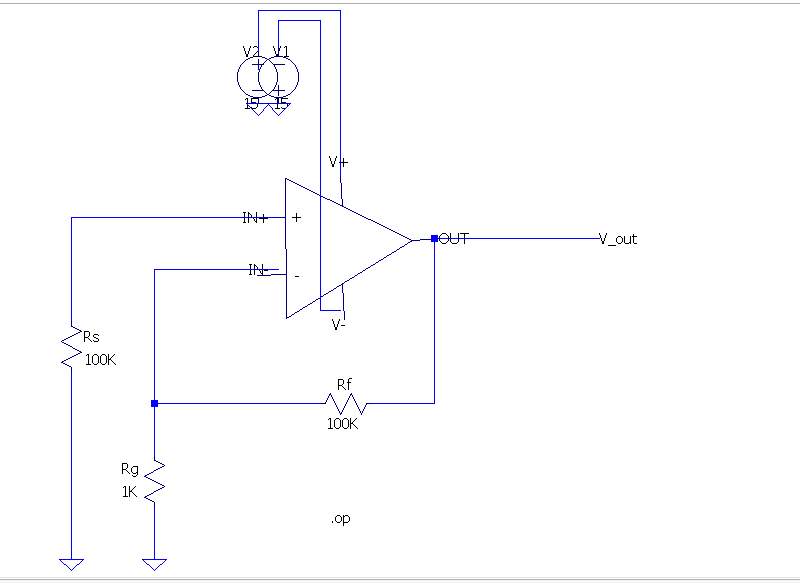
\includegraphics[width=0.75\textwidth]{imgs/simulacao/3.4circuitosimuladoTL064.png}
\caption{Simulação do circuito de corrente de polarização com o TL064.}
\label{fig:sim_polarizacao_tl064}
\end{figure}

\begin{figure}[H]
\centering
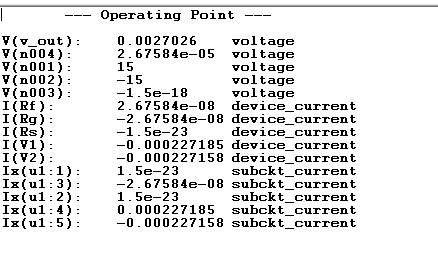
\includegraphics[width=0.75\textwidth]{imgs/simulacao/3.4resultadosimuladoTL064.png}
\caption{Resultados da simulação da corrente de polarização para o TL064.}
\label{fig:sim_res_polarizacao_tl064}
\end{figure}

\subsubsection{Resposta em frequência}

A resposta em frequência dos dois amplificadores não inversores foi simulada utilizando os valores reais dos resistores medidos em bancada. Para o estágio de ganho baixo, foram utilizados $R_f'=9{,}816~\mathrm{k}\Omega$ e $R_g'=807~\Omega$, resultando em

$$
G_{1,\mathrm{sim}}
=
1+\frac{9{,}816}{0{,}807}
\approx13{,}17.
$$

Para o estágio de ganho alto, foram utilizados $R_f=101~\mathrm{k}\Omega$ e $R_g=983~\Omega$, resultando em

$$
G_{2,\mathrm{sim}}
=
1+\frac{101}{0{,}983}
\approx103{,}75.
$$

\begin{figure}[H]
\centering
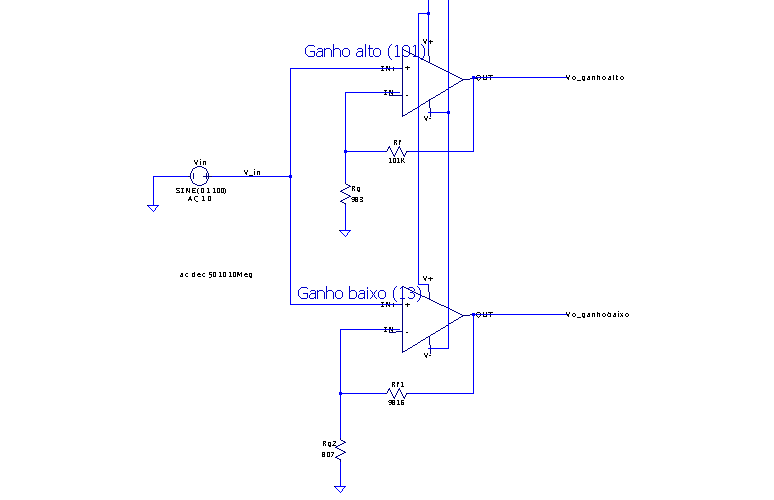
\includegraphics[width=0.80\textwidth]{imgs/simulacao/3.5circuitosimulado.png}
\caption{Circuito utilizado na simulação da resposta em frequência.}
\label{fig:sim_resposta_frequencia}
\end{figure}

O circuito está na Figura~\ref{fig:sim_resposta_frequencia}. A resposta em frequência simulada (Figura~\ref{fig:sim_gbw}) apresentou frequências de corte de aproximadamente $95{,}0~\mathrm{kHz}$ para o ganho baixo e $10{,}0~\mathrm{kHz}$ para o ganho alto.

Os respectivos produtos ganho--banda são

$$
GBW_1=G_{1,\mathrm{sim}}f_{c1}
=1{,}25\times 10^6~\mathrm{Hz}
$$

e

$$
GBW_2=G_{2,\mathrm{sim}}f_{c2}
=1{,}04\times 10^6~\mathrm{Hz}.
$$

\begin{figure}[H]
\centering
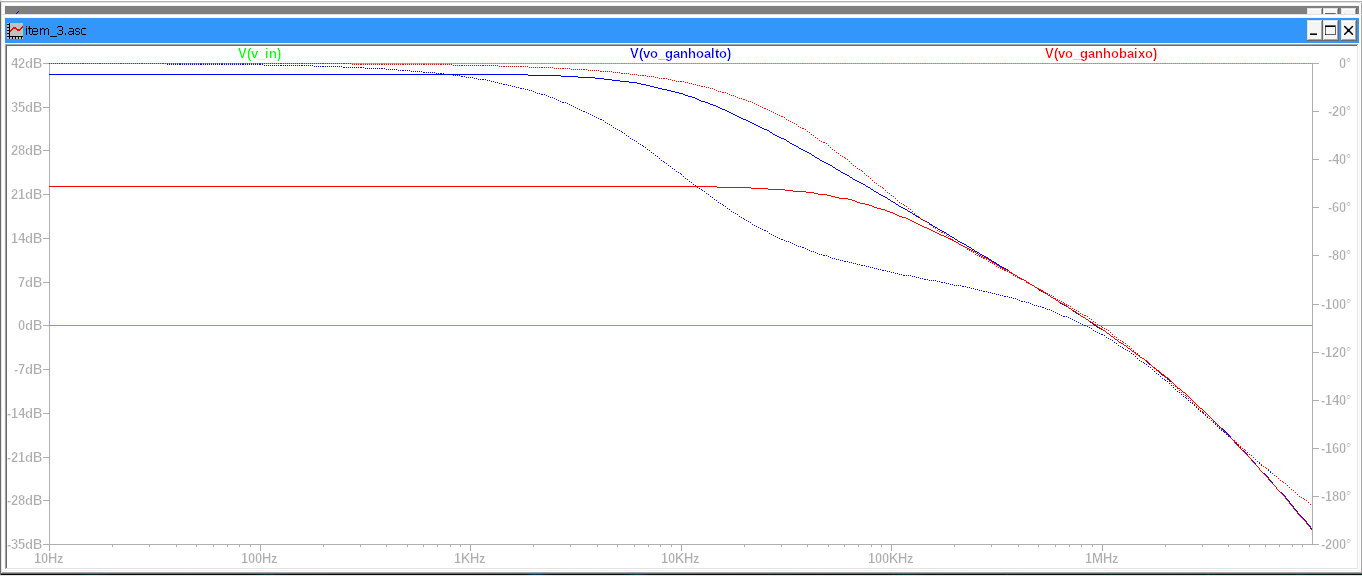
\includegraphics[width=0.85\textwidth]{imgs/simulacao/3.5resultadosimulado.png}
\caption{Resposta em frequência simulada dos estágios de ganho baixo e ganho alto.}
\label{fig:sim_gbw}
\end{figure}

\subsubsection{Slew rate}

O ensaio de \textit{slew rate} foi reproduzido no LTspice utilizando o LM741 configurado como seguidor de tensão e uma senoide com amplitude de pico $V_p=2{,}5$~V. A frequência foi variada para identificar a condição em que a saída deixa de acompanhar a forma senoidal e passa a apresentar comportamento aproximadamente triangular.

\begin{figure}[H]
\centering
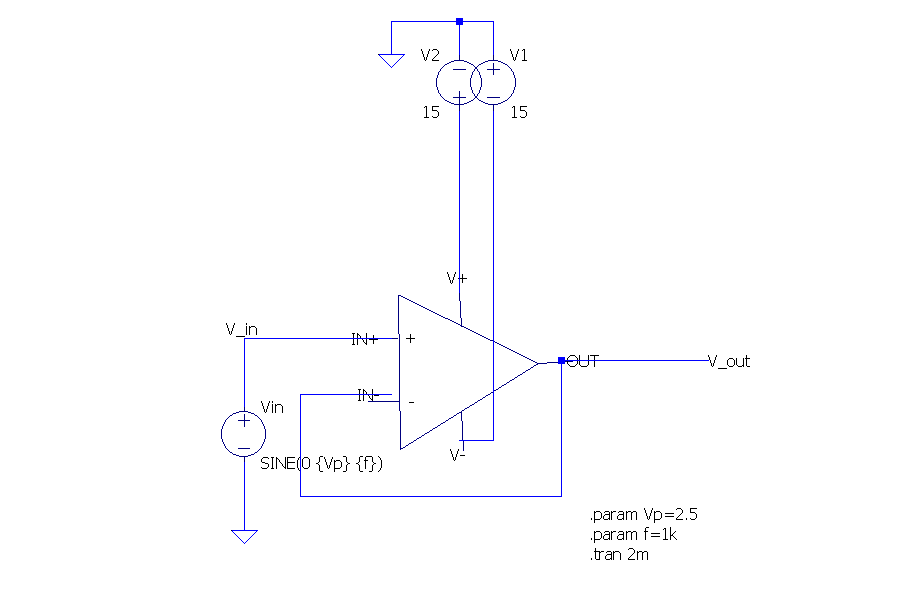
\includegraphics[width=0.80\textwidth]{imgs/simulacao/3.6circuitosimuladoLM741.png}
\caption{Simulação do circuito para o ensaio de \textit{slew rate} do LM741.}
\label{fig:sim_slew_lm741}
\end{figure}

O circuito está na Figura~\ref{fig:sim_slew_lm741}. As Figuras~\ref{fig:sim_slew_lm741_10hz} a~\ref{fig:sim_slew_lm741_1khz} mostram a saída para frequências de 10~Hz a 1~kHz:

\begin{figure}[H]
\centering
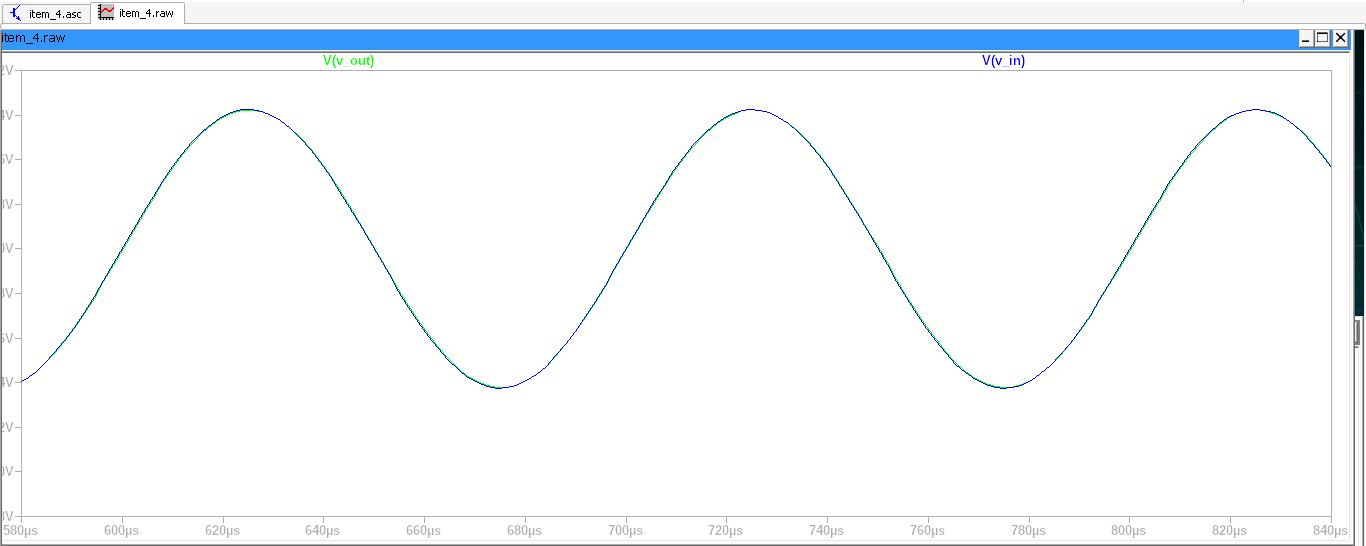
\includegraphics[width=0.80\textwidth]{imgs/simulacao/3.6resultadosimuladoLM74110Hz.png}
\caption{Simulação do \textit{slew rate} do LM741 a 10~Hz.}
\label{fig:sim_slew_lm741_10hz}
\end{figure}

\begin{figure}[H]
\centering
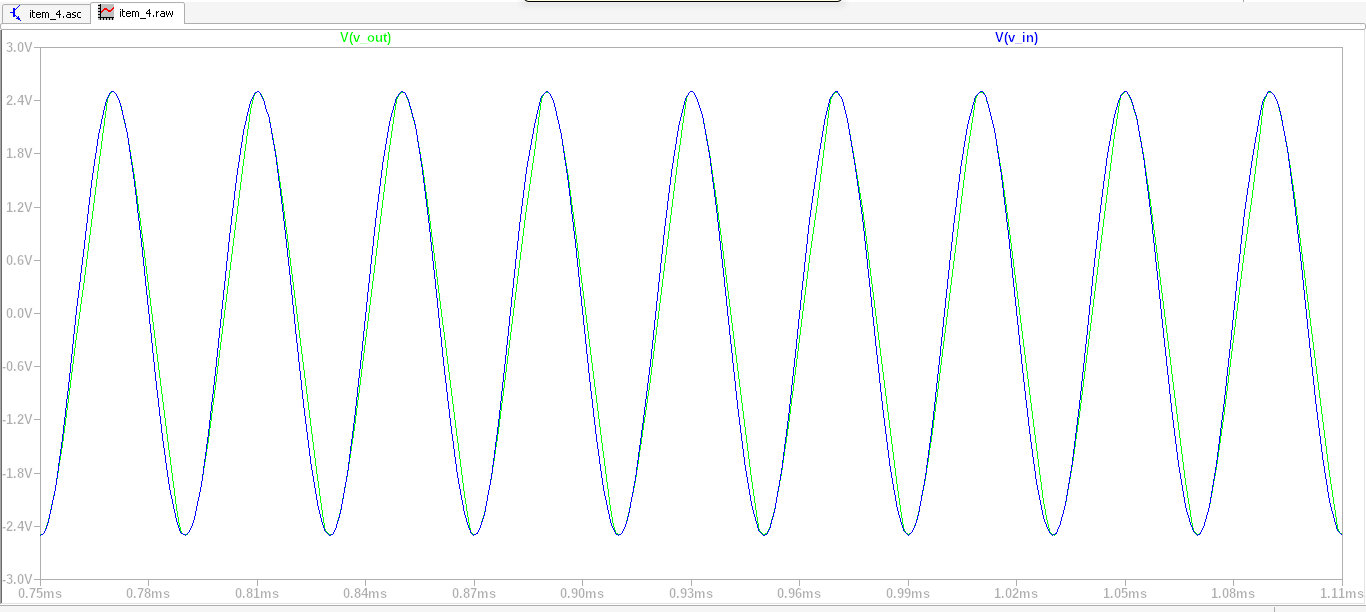
\includegraphics[width=0.80\textwidth]{imgs/simulacao/3.6resultadosimuladoLM74125Hz.png}
\caption{Simulação do \textit{slew rate} do LM741 a 25~Hz.}
\label{fig:sim_slew_lm741_25hz}
\end{figure}

\begin{figure}[H]
\centering
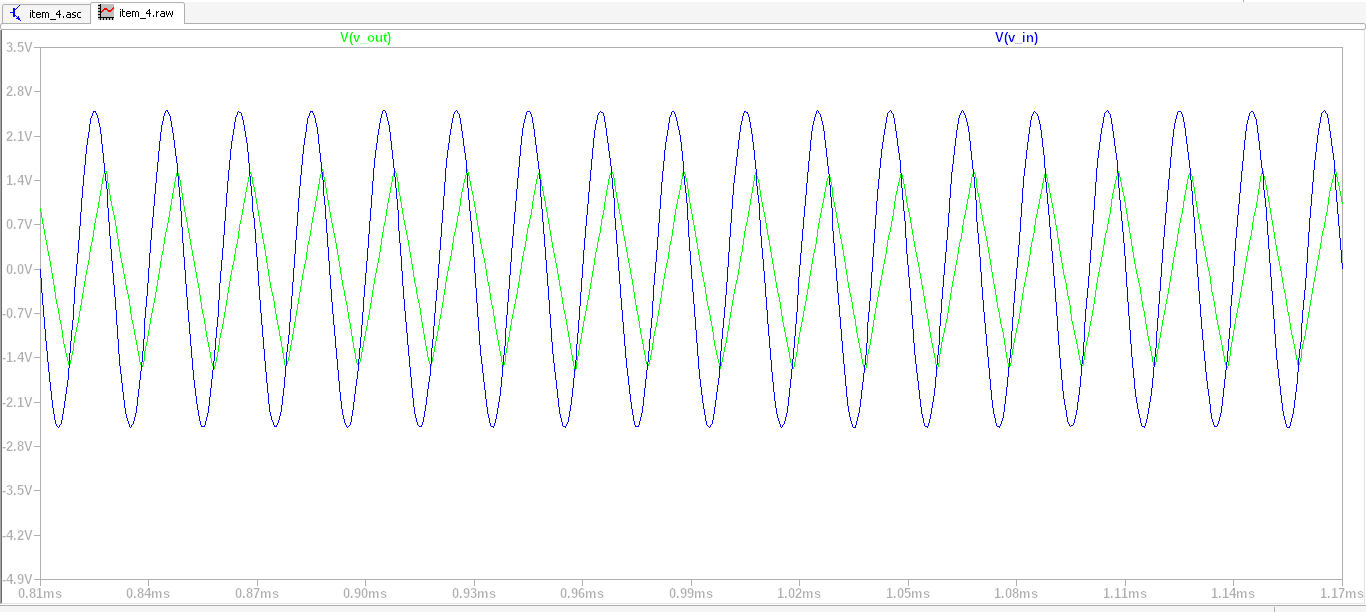
\includegraphics[width=0.80\textwidth]{imgs/simulacao/3.6resultadosimuladoLM74150Hz.png}
\caption{Simulação do \textit{slew rate} do LM741 a 50~Hz.}
\label{fig:sim_slew_lm741_50hz}
\end{figure}

\begin{figure}[H]
\centering
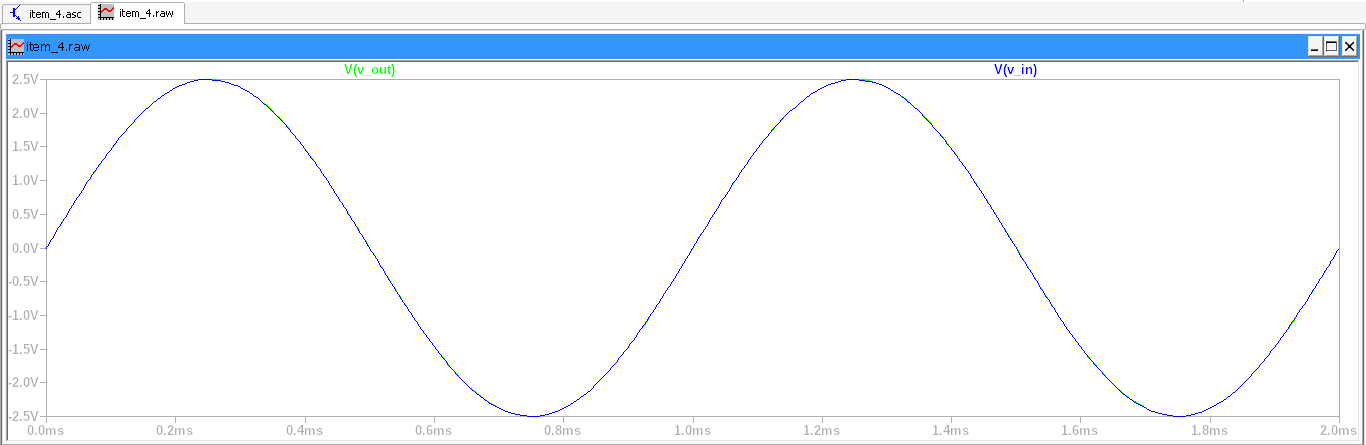
\includegraphics[width=0.80\textwidth]{imgs/simulacao/3.6resultadosimuladoLM7411kHz.png}
\caption{Simulação do \textit{slew rate} do LM741 a 1~kHz.}
\label{fig:sim_slew_lm741_1khz}
\end{figure}

Nas quatro frequências a saída acompanha a senoide de entrada, o que é esperado: todas estão abaixo de $f_{\mathrm{SR}}=SR/(2\pi V_p)\approx20$~kHz, calculado com o \textit{slew rate} do modelo ($\approx0{,}32$~V/$\mu$s, Seção~5.1). Essas simulações confirmam o regime linear em baixa frequência, mas não fornecem o \textit{slew rate}. Como o seguidor não tem resistores, a tolerância dos componentes não entra nesse ensaio, e o \textit{slew rate} das simulações de projeto (Seção~5.1) vale também para a montagem.

Para o TL064, o mesmo procedimento foi repetido utilizando o modelo correspondente (Figuras~\ref{fig:sim_slew_tl064} e~\ref{fig:sim_res_slew_tl064}).

\begin{figure}[H]
\centering
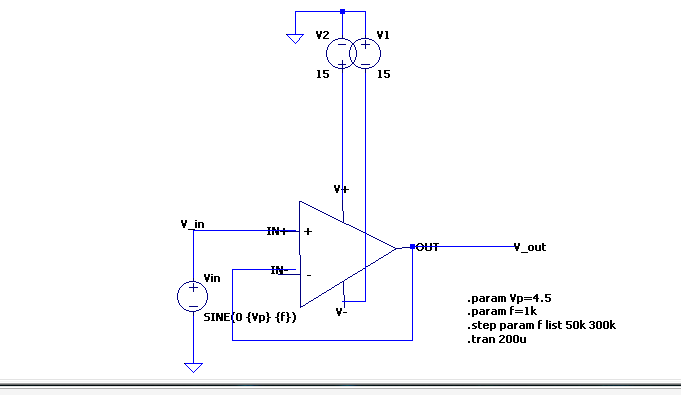
\includegraphics[width=0.80\textwidth]{imgs/simulacao/3.6circuitosimuladoTL064.png}
\caption{Simulação do circuito para o ensaio de \textit{slew rate} do TL064.}
\label{fig:sim_slew_tl064}
\end{figure}

\begin{figure}[H]
\centering
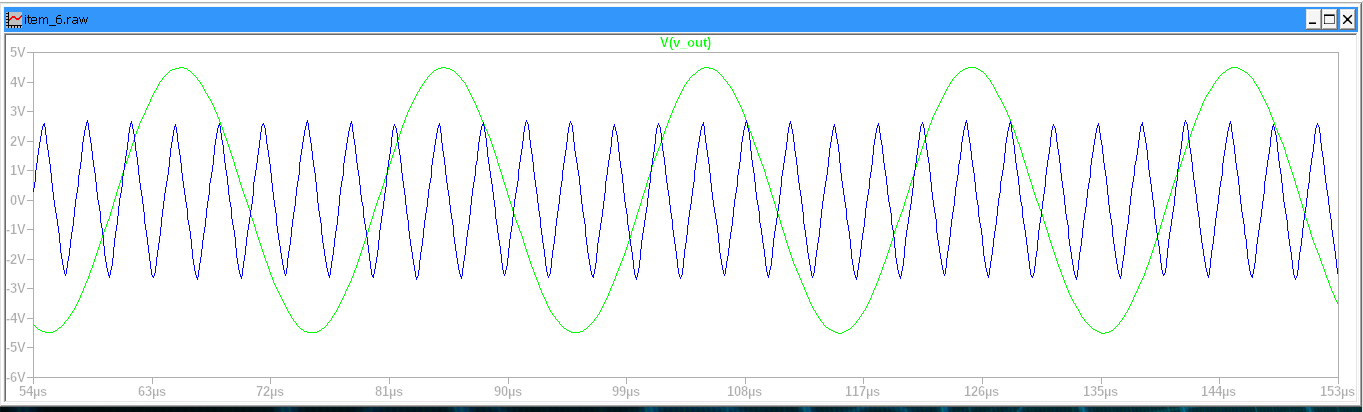
\includegraphics[width=0.80\textwidth]{imgs/simulacao/3.6resultadosimuladoTL064.png}
\caption{Simulação do \textit{slew rate} do TL064.}
\label{fig:sim_res_slew_tl064}
\end{figure}

Para uma senoide de amplitude $V_p=2{,}5$~V, a frequência limite associada ao \textit{slew rate} pode ser obtida por

$$
f_{\mathrm{SR}}=\frac{SR}{2\pi V_p}.
$$

Os valores de simulação são confrontados com a bancada e com os \textit{datasheets} na Seção~6.
\section{Resultados}

\subsection{Projeto de cada integrante}

\subsubsection{Guilherme Cardoso Oliveira da Silva Júnior (23/1038626)}

A Tabela~\ref{tab:resultados_cardoso} apresenta os parâmetros de não idealidades em corrente contínua (tensão de offset e corrente de polarização) calculados analiticamente a partir dos pontos de operação (\texttt{.op}) simulados no LTspice.

\begin{table}[H]
    \centering
    \caption{Resultados simulados de tensão de offset e corrente de polarização (Matrícula 23/1038626).}
    \label{tab:resultados_cardoso}
    \renewcommand{\arraystretch}{1.2}
    \begin{tabular}{@{}lrrr@{}}
    \toprule
    \textbf{Grandeza} & \textbf{Analítico (E12)} & \textbf{Simulado} & \textbf{Erro (\%)} \\
    \midrule    
    Ganho $G_1$ & $36{,}87$ & $36{,}86$ & $0{,}03\%$ \\
    Ganho $G_2$ & $101{,}00$ & $100{,}95$ & $0{,}05\%$ \\
    Tensão de Offset $V_{os}$ (LM741)* & $1{,}00\text{ mV}$ & $1{,}10\text{ mV}$ & $10{,}00\%$ \\
    Corrente de Polarização $I_b$ (LM741)* & $80{,}00\text{ nA}$ & $57{,}82\text{ nA}$ & $27{,}73\%$ \\
    \textit{Slew Rate} (LM741)* & $0{,}50\text{ V/}\mu\text{s}$ & $0{,}315\text{ V/}\mu\text{s}$ & $37{,}00\%$ \\
    \textit{Slew Rate} (TL064)* & $3{,}00\text{ V/}\mu\text{s}$ & $3{,}286\text{ V/}\mu\text{s}$ & $9{,}53\%$ \\
    \bottomrule
    \multicolumn{4}{l}{\footnotesize * Para as grandezas não ideais, o valor analítico reflete o típico de \textit{datasheet}.}
    \end{tabular}
\end{table}

\paragraph{Análise Analítica DC:}
A tensão de offset do LM741 foi calculada refletindo a tensão de saída para a entrada do amplificador não inversor de ganho 101, resultando em $V_{os}=\frac{111{,}13\text{ mV}}{101}=1{,}10\text{ mV}$. Este valor encontra-se perfeitamente dentro da faixa típica informada no \textit{datasheet} do componente. 

A corrente de polarização foi determinada através da variação da tensão de saída ($\Delta V_o$) ao inserir o resistor $R_s=100\text{ k}\Omega$. Para o LM741, a diferença foi de $\Delta V_o=|-472{,}85\text{ mV}-111{,}13\text{ mV}|=583{,}98\text{ mV}.$ Pela relação $I_b=\frac{\Delta V_o}{101 \cdot R_s}$, obteve-se $I_b=57{,}82\text{ nA}$, compatível com a tecnologia bipolar do AmpOp. O mesmo procedimento aplicado ao TL064 (tecnologia JFET) resultou uma variação de saída quase nula, comprovando que a sua corrente  de polarização é na ordem dos picoamperes (pA), sendo desprezível na simulação e resultando numa razão $\frac{I_{b(LM741)}}{I_{b(TL064)}} \to \infty$.

A Figura~\ref{fig:graficos_cardoso} exibe as formas de onda resultantes das simulações dinâmicas em frequência (\texttt{.ac}) e de regime transiente (\texttt{.tran}), evidenciando as limitações de largura de banda para os diferentes ganhos e as distorções causadas pela taxa de subida (\textit{slew rate}).

\begin{figure}[H]
    \centering
    \begin{minipage}[b]{0.48\linewidth}
        \centering
        \includegraphics[width=\linewidth]{imgs/cardoso/cardoso_resultados/simulação_item_3_ganho_g1.png}
        \vspace{2pt}
        {\small (a) Resposta em Frequência (Ganho $G_1=37)$.}
    \end{minipage}%
    \hfill
    \begin{minipage}[b]{0.48\linewidth}
        \centering
        \includegraphics[width=\linewidth]{imgs/cardoso/cardoso_resultados/simulação_item_3_ganho_g2.png}
        \vspace{2pt}
        {\small (b) Resposta em Frequência (Ganho $G_2=101$).}
    \end{minipage}

    \vspace{12pt}

    \begin{minipage}[b]{0.48\linewidth}
        \centering
        \includegraphics[width=\linewidth]{imgs/cardoso/cardoso_resultados/simulação_item_4_slew_rate_LM741.png}
        \vspace{2pt}
        {\small (c) \textit{Slew Rate} (LM741).}
    \end{minipage}
    \hfill
    \begin{minipage}[b]{0.48\linewidth}
        \centering
        \includegraphics[width=\linewidth]{imgs/cardoso/cardoso_resultados/simulação_item_6_slew_rate_TL064.png}
        \vspace{2pt}
        {\small (d) \textit{Slew Rate} (TL064).}
    \end{minipage}
    \caption{Resultados gráficos das simulações de projeto (matrícula 23/1038626).}
    \label{fig:graficos_cardoso}
\end{figure}

\paragraph{Análise Analítica AC e Transiente:}
A partir das curvas de resposta em frequência (Figuras~\ref{fig:graficos_cardoso}a e \ref{fig:graficos_cardoso}b), determinou-se analiticamente  o Produto Ganho-Banda (GBW) de cada configuração. Para o ganho real de malha fechada $G_1=37$ (realizado com a associação de resistores da série E12 resultando numa proporção de $36{,}87$), a frequência de corte a $-3\text{ dB}$ medida foi de $f_{c1} \approx 26{,}95\text{ kHz}$, o que acarreta num produto $GBW_1=36{,}86 \times 26{,}95\text{ kHz} \approx 993{,}3\text{ kHz}$. Para o ganho $G_2=101$, obteve-se $f_{c2} \approx 9{,}82\text{ kHz}$, gerando um produto $GBW=100{,}95 \times 9{,}82\text{ kHz} \approx 991{,}3\text{ kHz}$.

No que tange à distorção por \textit{Slew Rate} (SR), o limite de frequência teórica a partir da qual uma senoide de amplitude $V_p = 5\text{ V}$ sofre ceifamento triangular é calculado por $f_{max} = \frac{SR}{2\pi V_p}$. Através da inclinação da rampa medida com os cursores no LTspice, o SR simulado do LM741 foi de $0{,}315\text{ V/}\mu\text{s}$, projetando uma distorção limite a partir de $f_{max} \approx 10{,}0\text{ kHz}$. Em contrapartida, a medição da rampa para o TL064 resultou num SR de $3{,}286\text{ V/}\mu\text{s}$ (próximo aos $3{,}0\text{ V/}\mu\text{s}$ nominais de \textit{datasheet}), o que eleva a frequência máxima sem distorção para $f_{max} \approx 104{,}6\text{ kHz}$. A comparação evidencia de forma prática que o modelo JFET (TL064) é substancialmente mais veloz que o modelo bipolar (LM741) para lidar com variações abruptas de tensão. 

\subsubsection{Daniel Campos Silva (23/1036775)}

A Tabela~\ref{tab:resultados_daniel} apresenta os parâmetros de não idealidades em corrente contínua (tensão de offset e corrente de polarização) calculados analiticamente a partir dos pontos de operação (\texttt{.op}) simulados no LTspice.

\begin{table}[H]
    \centering
    \caption{Resultados simulados de tensão de offset e corrente de polarização (Matrícula 23/1036775).}
    \label{tab:resultados_daniel}
    \renewcommand{\arraystretch}{1.2}
    \begin{tabular}{@{}lrrr@{}}
    \toprule
    \textbf{Grandeza} & \textbf{Analítico (E12)} & \textbf{Simulado} & \textbf{Erro (\%)} \\
    \midrule    
    Ganho $G_1$ & $35{,}00$ & $35{,}02$ & $0{,}06\%$ \\
    Ganho $G_2$ & $116{,}00$ & $115{,}88$ & $0{,}10\%$ \\
    Tensão de Offset $V_{os}$ (LM741)* & $1{,}00\text{ mV}$ & $1{,}21\text{ mV}$ & $21{,}00\%$ \\
    Corrente de Polarização $I_b$ (LM741)* & $80{,}00\text{ nA}$ & $68{,}04\text{ nA}$ & $14{,}95\%$ \\
    \textit{Slew Rate} (LM741)* & $0{,}50\text{ V/}\mu\text{s}$ & $0{,}320\text{ V/}\mu\text{s}$ & $36{,}00\%$ \\
    \textit{Slew Rate} (TL064)* & $3{,}00\text{ V/}\mu\text{s}$ & $3{,}250\text{ V/}\mu\text{s}$ & $8{,}33\%$ \\
    \bottomrule
    \multicolumn{4}{l}{\footnotesize * Para as grandezas não ideais, o valor analítico reflete o típico de \textit{datasheet}.}
    \end{tabular}
\end{table}

\paragraph{Análise Analítica DC:}
A tensão de offset do LM741 foi calculada refletindo a tensão de saída para a entrada do amplificador não inversor de ganho $101$ ($R_f=100\text{ k}\Omega$ e $R_g=1\text{ k}\Omega$, Figura~\ref{fig:circs_daniel}a), resultando em $V_{os}=\frac{121{,}80\text{ mV}}{101}=1{,}21\text{ mV}$. Este valor encontra-se perfeitamente dentro da faixa típica informada no \textit{datasheet} do componente. 

A corrente de polarização foi determinada através da variação da tensão de saída ($\Delta V_o$) ao inserir o resistor $R_s=100\text{ k}\Omega$. Para o LM741, a diferença medida foi de $\Delta V_o=|-565{,}40\text{ mV}-121{,}80\text{ mV}|=687{,}20\text{ mV}.$ Pela relação $I_b=\frac{\Delta V_o}{101 \cdot R_s}$, obteve-se $I_b=68{,}04\text{ nA}$, compatível com a tecnologia bipolar do AmpOp. O mesmo procedimento aplicado ao TL064 (tecnologia JFET) resultou em uma variação de saída quase nula, comprovando que a sua corrente de polarização é da ordem dos picoamperes (pA), sendo desprezível na simulação e resultando numa razão $\frac{I_{b(LM741)}}{I_{b(TL064)}} \to \infty$.

A Figura~\ref{fig:graficos_daniel} exibe as formas de onda resultantes das simulações dinâmicas em frequência (\texttt{.ac}) e de regime transiente (\texttt{.tran}), evidenciando as limitações de largura de banda para os diferentes ganhos e as distorções causadas pela taxa de subida (\textit{slew rate}).

\begin{figure}[H]
    \centering
    \begin{minipage}[b]{0.48\linewidth}
        \centering
        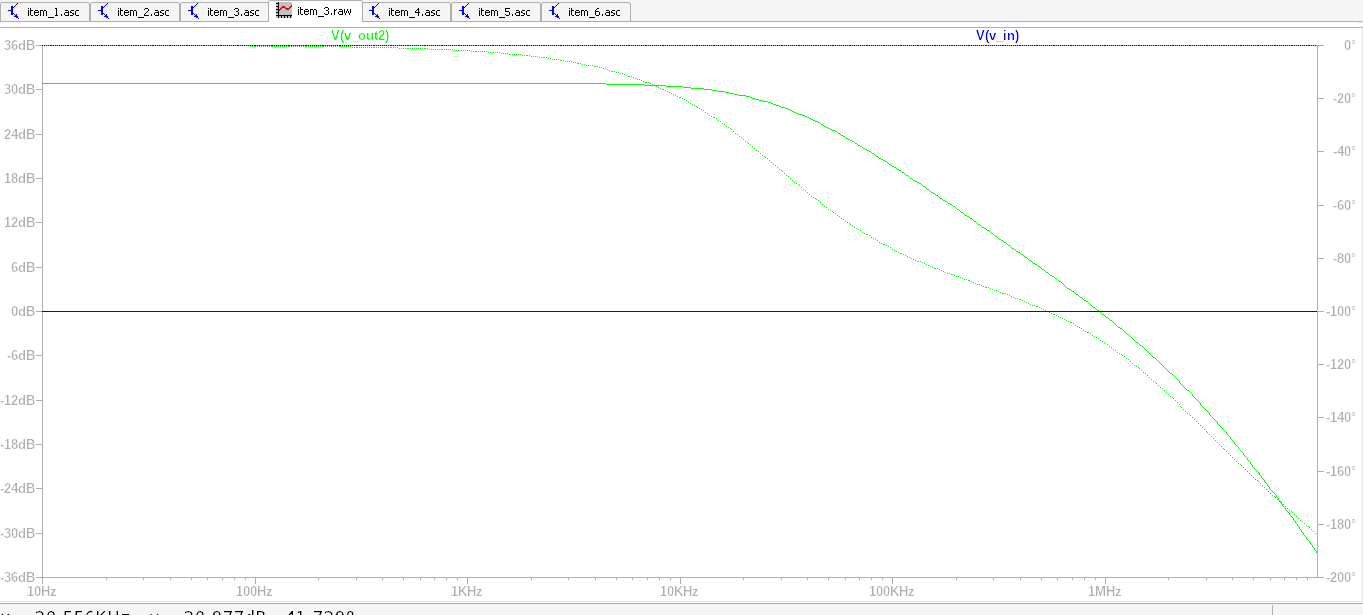
\includegraphics[width=\linewidth]{imgs/daniel/daniel_resultados/simulacao_item_3_ganho_g1.png}
        \vspace{2pt}
        {\small (a) Resposta em Frequência (Ganho $G_1=35$).}
    \end{minipage}%
    \hfill
    \begin{minipage}[b]{0.48\linewidth}
        \centering
        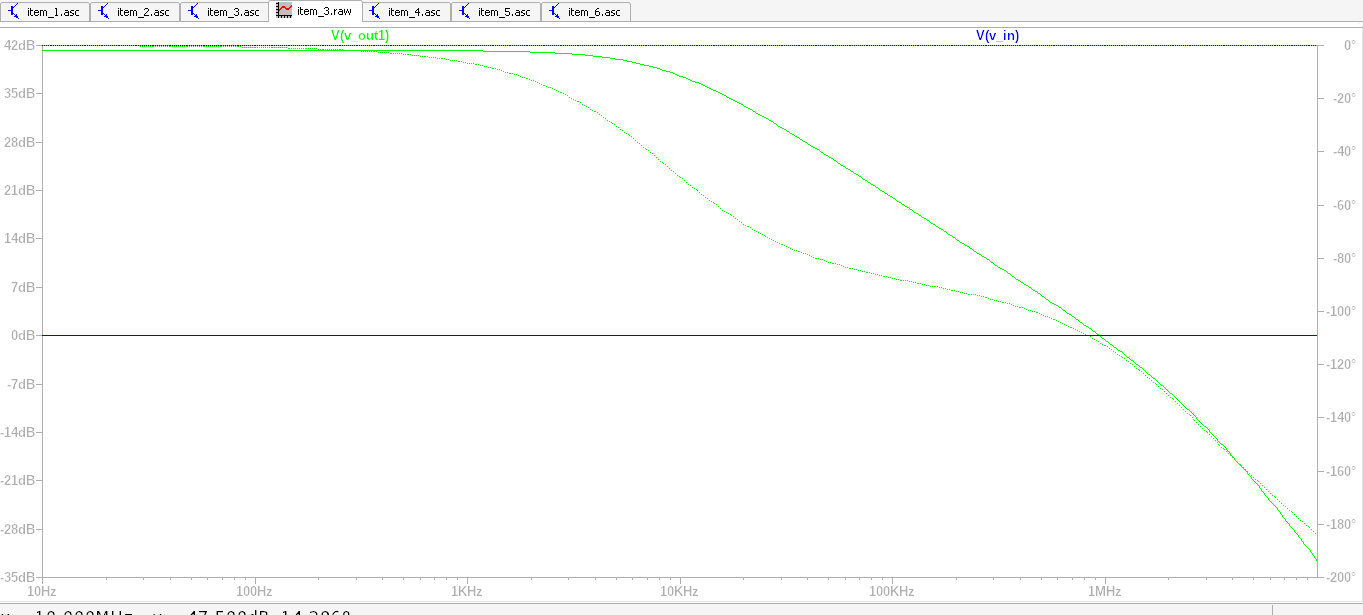
\includegraphics[width=\linewidth]{imgs/daniel/daniel_resultados/simulacao_item_3_ganho_g2.png}
        \vspace{2pt}
        {\small (b) Resposta em Frequência (Ganho $G_2=116$).}
    \end{minipage}

    \vspace{12pt}

    \begin{minipage}[b]{0.48\linewidth}
        \centering
        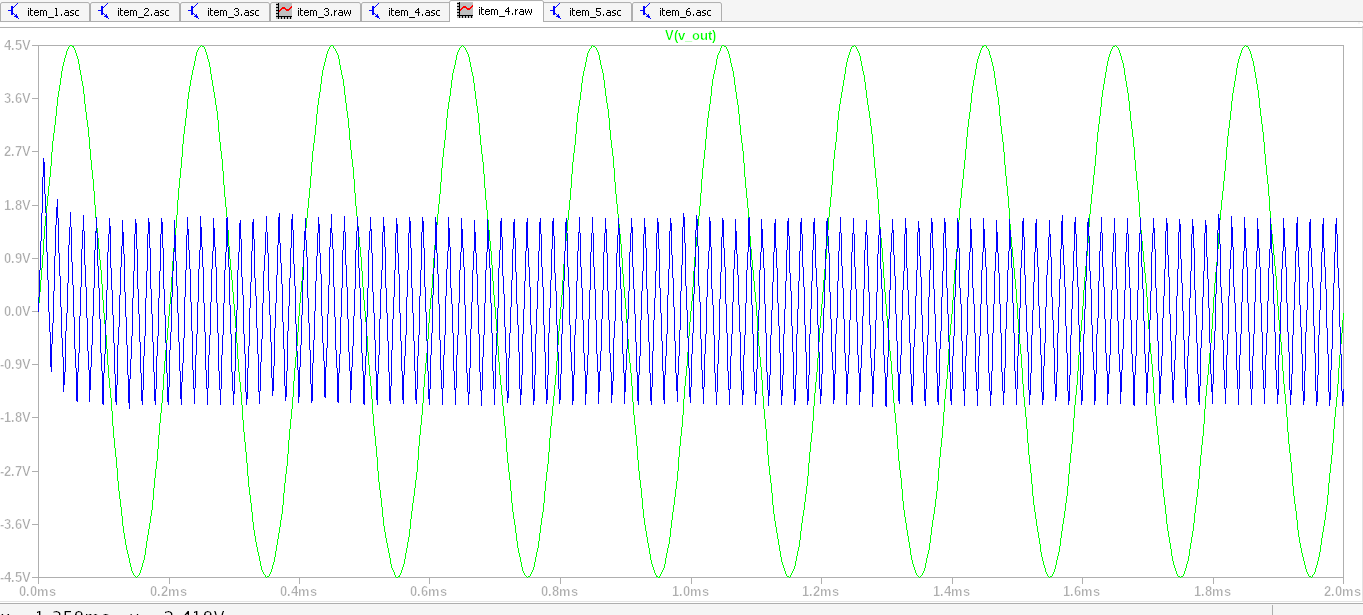
\includegraphics[width=\linewidth]{imgs/daniel/daniel_resultados/simulacao_item_4_slew_rate_LM741.png}
        \vspace{2pt}
        {\small (c) \textit{Slew Rate} (LM741).}
    \end{minipage}
    \hfill
    \begin{minipage}[b]{0.48\linewidth}
        \centering
        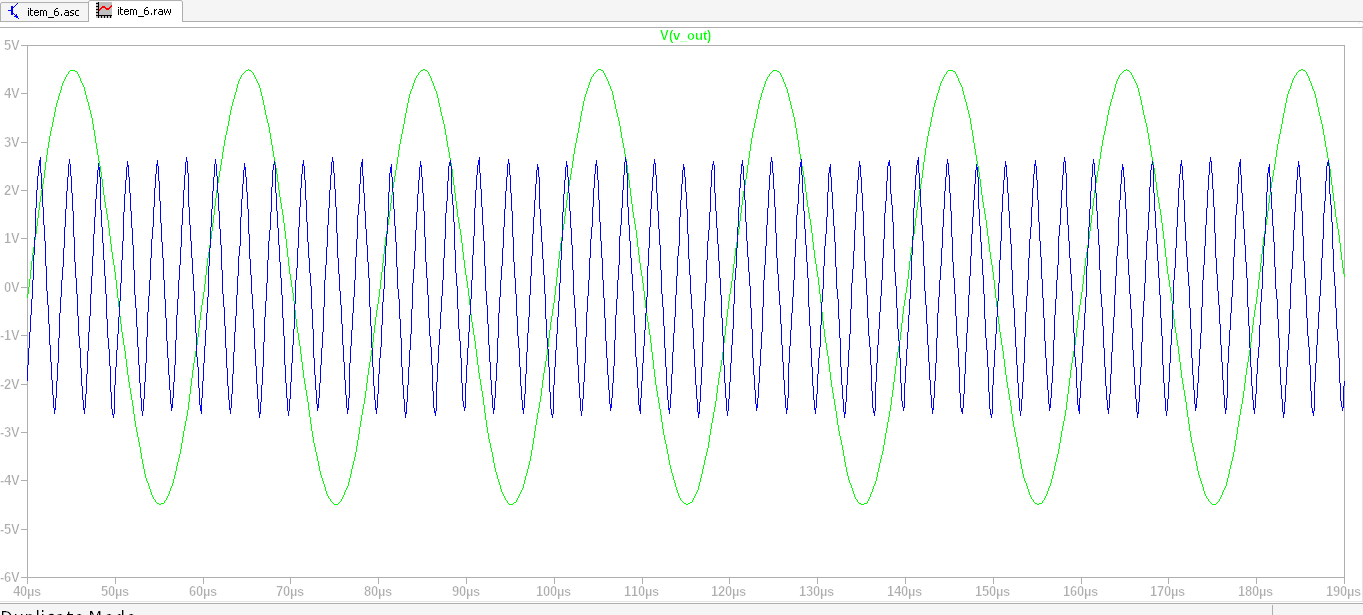
\includegraphics[width=\linewidth]{imgs/daniel/daniel_resultados/simulacao_item_6_slew_rate_TL064.png}
        \vspace{2pt}
        {\small (d) \textit{Slew Rate} (TL064).}
    \end{minipage}
    \caption{Resultados gráficos das simulações de projeto (matrícula 23/1036775).}
    \label{fig:graficos_daniel}
\end{figure}

\paragraph{Análise Analítica AC e Transiente:}
A partir das curvas de resposta em frequência (Figuras~\ref{fig:graficos_daniel}a e \ref{fig:graficos_daniel}b), determinou-se analiticamente o Produto Ganho-Banda (GBW) de cada configuração. Para o ganho real de malha fechada $G_1=35$ (realizado com os resistores $R_g = 1{,}5\text{ k}\Omega$ e $R_f = 51\text{ k}\Omega$), a frequência de corte a $-3\text{ dB}$ medida foi de $f_{c1} \approx 28{,}45\text{ kHz}$, o que acarreta em um produto $GBW_1=35{,}02 \times 28{,}45\text{ kHz} \approx 996{,}3\text{ kHz}$. Para o ganho $G_2=116$ (utilizando $R_g = 1\text{ k}\Omega$ e $R_f = 115\text{ k}\Omega$), obteve-se $f_{c2} \approx 8{,}62\text{ kHz}$, gerando um produto $GBW_2=115{,}88 \times 8{,}62\text{ kHz} \approx 998{,}9\text{ kHz}$.

No que tange à distorção por \textit{Slew Rate} (SR), o limite de frequência teórica a partir da qual uma senoide de amplitude $V_p = 4{,}5\text{ V}$ sofre ceifamento triangular é calculado por $f_{max} = \frac{SR}{2\pi V_p}$. Através da inclinação da rampa medida com os cursores no LTspice, o SR simulado do LM741 foi de $0{,}320\text{ V/}\mu\text{s}$, projetando uma distorção limite a partir de $f_{max} \approx 11{,}32\text{ kHz}$. Em contrapartida, a medição da rampa para o TL064 resultou em um SR de $3{,}250\text{ V/}\mu\text{s}$ (próximo aos $3{,}0\text{ V/}\mu\text{s}$ nominais de \textit{datasheet}), o que eleva a frequência máxima sem distorção para $f_{max} \approx 114{,}9\text{ kHz}$. A comparação evidencia de forma prática que o modelo JFET (TL064) é substancialmente mais veloz que o modelo bipolar (LM741) para lidar com variações abruptas de tensão.

\subsubsection{Lurian Correia Lima (22/2005395)}

A Figura~\ref{fig:graficos_luri} reúne as simulações dinâmicas do projeto: as respostas em frequência dos dois ganhos com o LM741 e os ensaios de \textit{slew rate} do LM741 e do TL064.

\begin{figure}[H]
    \centering
    \begin{minipage}[b]{0.48\linewidth}
        \centering
        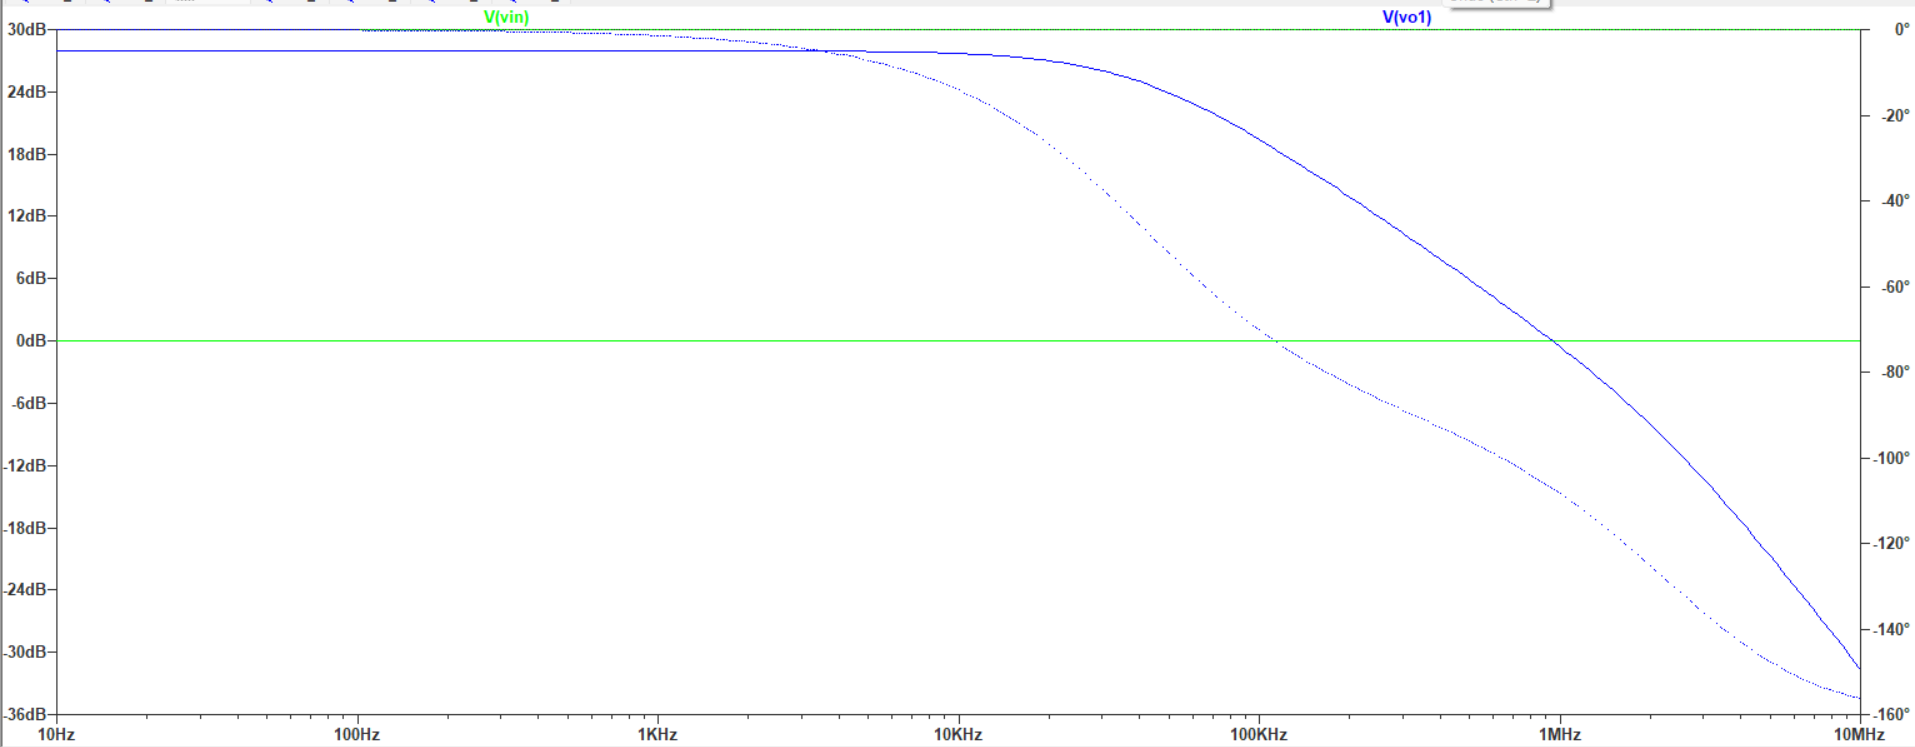
\includegraphics[width=\linewidth]{imgs/luri/resultados/Resposta em frequencia LM741(g25).png}
        \vspace{2pt}
        {\small (a) Resposta em frequência (ganho $G_1=25$).}
    \end{minipage}%
    \hfill
    \begin{minipage}[b]{0.48\linewidth}
        \centering
        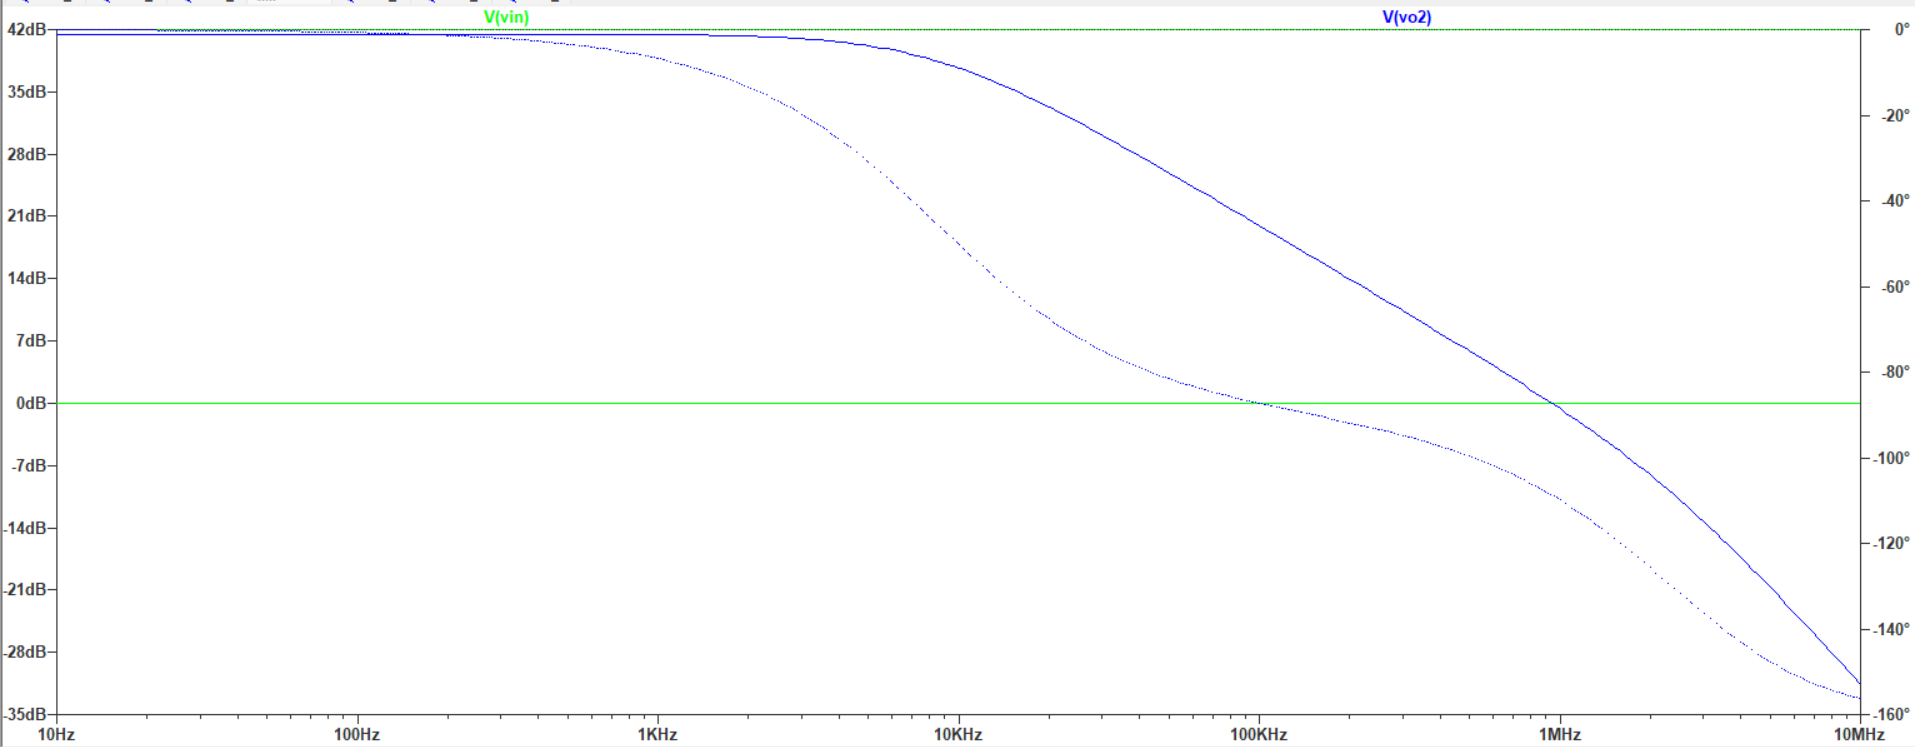
\includegraphics[width=\linewidth]{imgs/luri/resultados/Resposta em frequencia LM741(g119).png}
        \vspace{2pt}
        {\small (b) Resposta em frequência (ganho $G_2=119$).}
    \end{minipage}

    \vspace{12pt}

    \begin{minipage}[b]{0.48\linewidth}
        \centering
        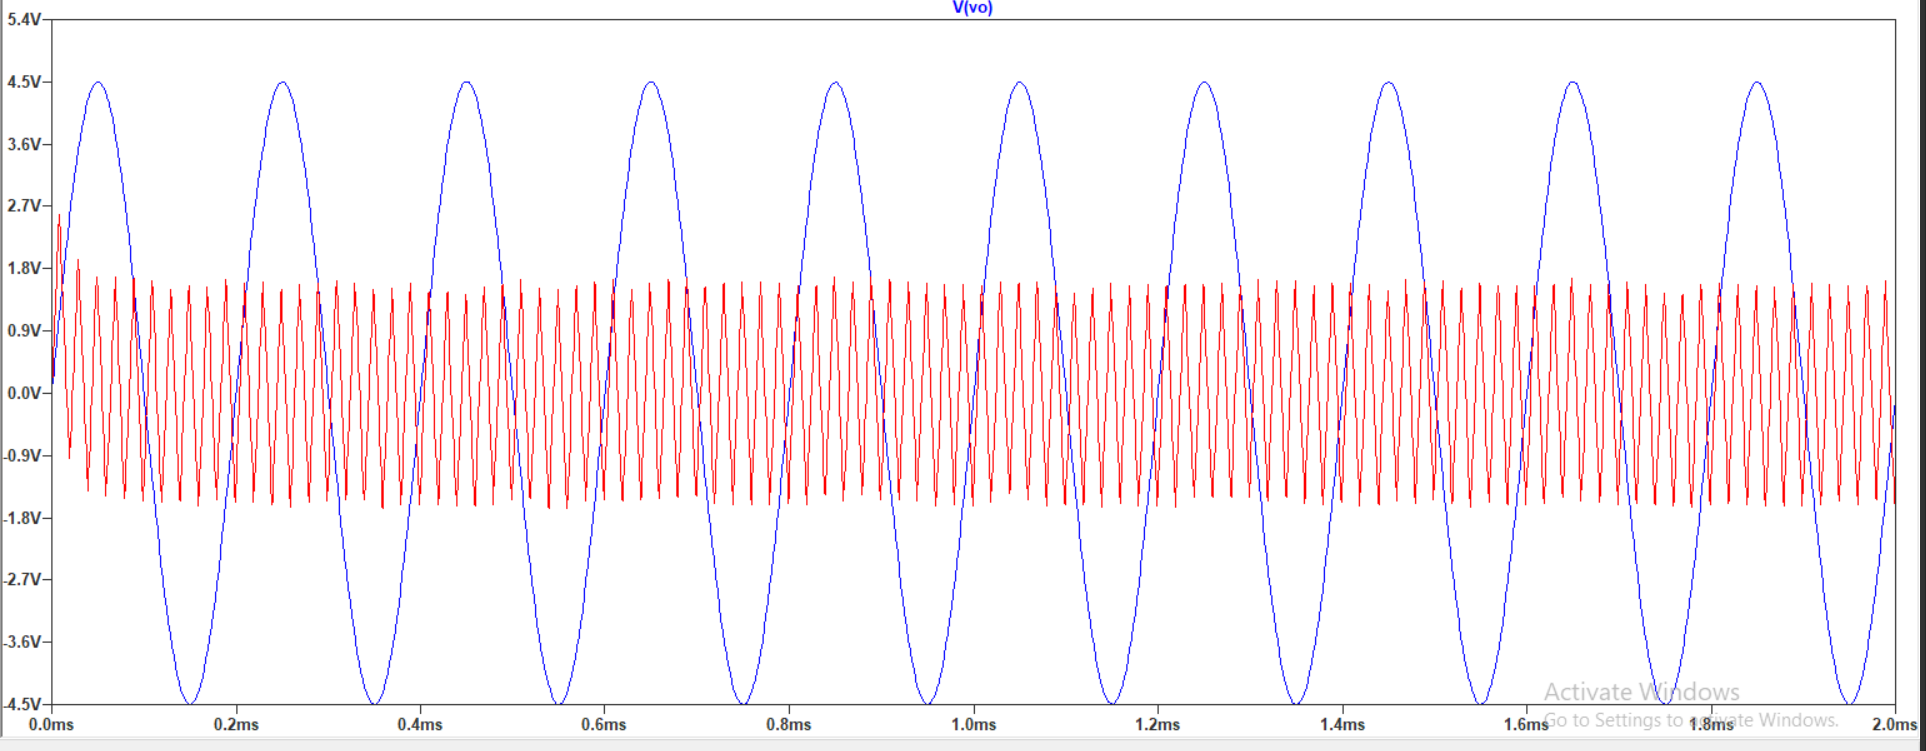
\includegraphics[width=\linewidth]{imgs/luri/resultados/slew_rate_lm741.png}
        \vspace{2pt}
        {\small (c) \textit{Slew rate} (LM741), 5~kHz e 50~kHz.}
    \end{minipage}
    \hfill
    \begin{minipage}[b]{0.48\linewidth}
        \centering
        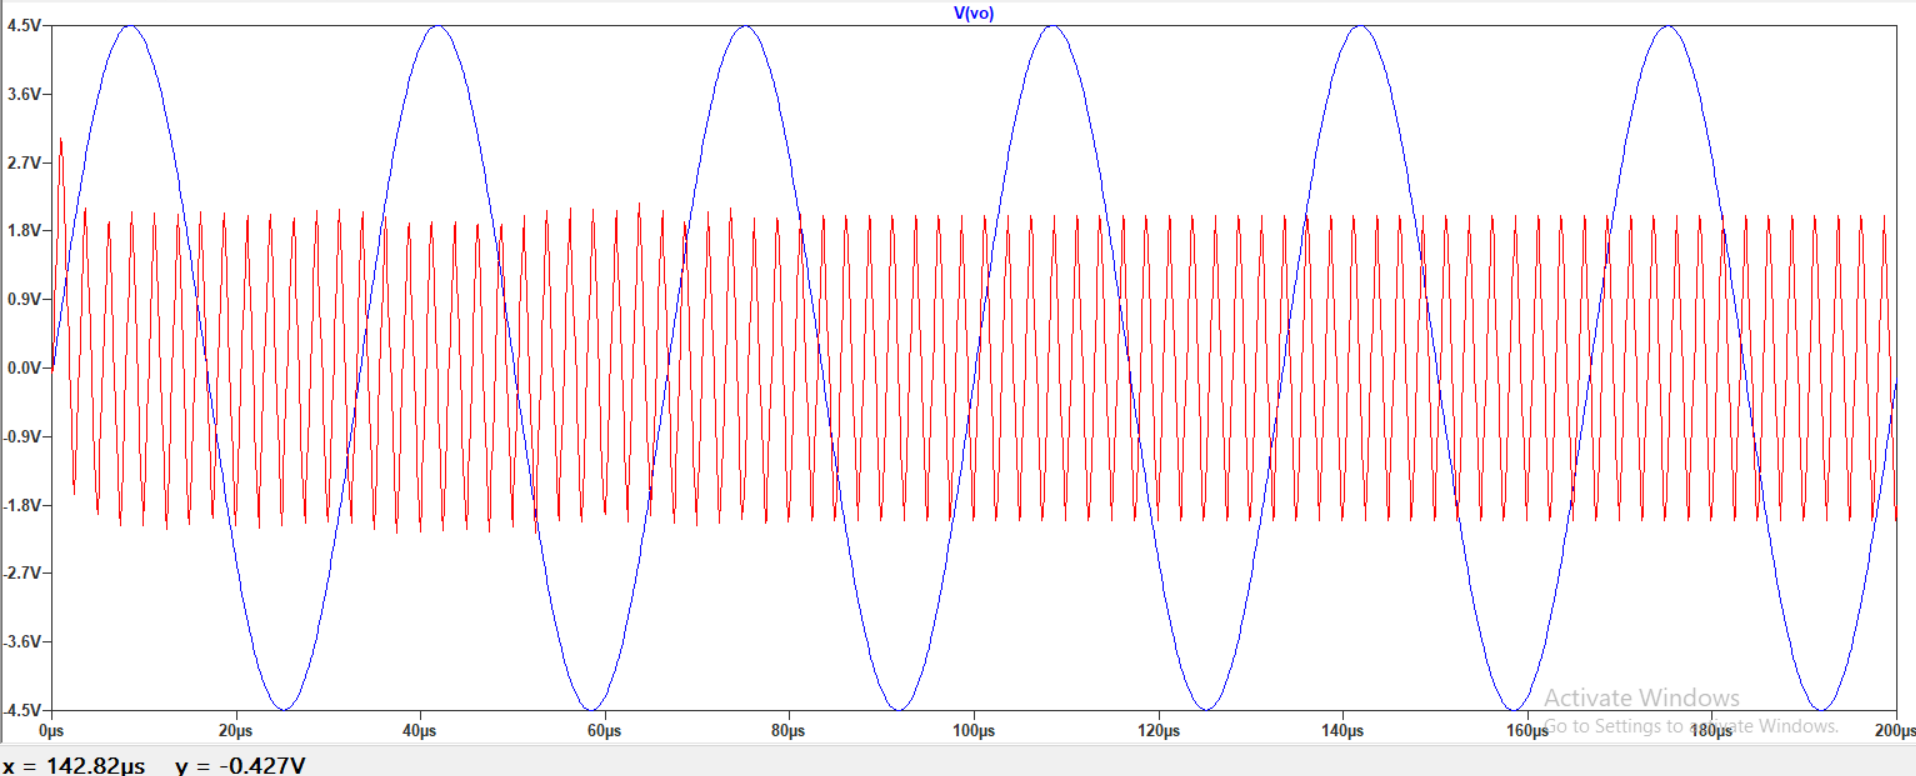
\includegraphics[width=\linewidth]{imgs/luri/resultados/slew_rate_tl064.png}
        \vspace{2pt}
        {\small (d) \textit{Slew rate} (TL064), 30~kHz e 400~kHz.}
    \end{minipage}
    \caption{Resultados gráficos das simulações de projeto (matrícula 22/2005395).}
    \label{fig:graficos_luri}
\end{figure}

\paragraph{Análise AC:}
Nas Figuras~\ref{fig:graficos_luri}a e \ref{fig:graficos_luri}b, o patamar de baixa frequência está em cerca de $28\text{ dB}$ para $G_1=25$ e em cerca de $41{,}5\text{ dB}$ para $G_2=119$, o que corresponde aos ganhos realizados de $1+24/1=25$ e $1+118/1=119$. A frequência de corte de $-3\text{ dB}$, lida nas curvas, ficou em torno de $40\text{ kHz}$ para o ganho baixo e de $8\text{ kHz}$ para o ganho alto. As duas curvas de módulo cruzam $0\text{ dB}$ praticamente no mesmo ponto, perto de $1\text{ MHz}$, e a fase passa por $-45^\circ$ nas respectivas frequências de corte, como esperado para um polo dominante. Os produtos ganho-banda ficam então em $25\times40\text{ kHz}\approx119\times8\text{ kHz}\approx1\text{ MHz}$, o que concorda com o valor obtido pelos outros integrantes ($\approx 1\text{ MHz}$) e confirma $f_c\approx \mathrm{GBW}/G$. Esses valores foram lidos graficamente, sem cursores, e por isso carregam a incerteza da leitura.

\paragraph{Análise do \textit{slew rate}:}
Com $V_p=4{,}5\text{ V}$, o limite teórico de frequência sem distorção é $f_{max}=\mathrm{SR}/(2\pi V_p)$. Nas Figuras~\ref{fig:graficos_luri}c e \ref{fig:graficos_luri}d, a senoide de frequência baixa (5~kHz no LM741 e 30~kHz no TL064) é reproduzida na saída com os $4{,}5\text{ V}$ de pico, ou seja, o amplificador acompanha o sinal. Na frequência alta (50~kHz no LM741 e 400~kHz no TL064), a saída vira um triângulo de amplitude muito menor que a da entrada, e a inclinação da rampa passa a ser o \textit{slew rate} do componente. Para um triângulo de pico $A$ e frequência $f$, a rampa sobe $2A$ em meio período, de modo que $\mathrm{SR}=4fA$.

No LM741, o triângulo tem pico de aproximadamente $1{,}6\text{ V}$ a $50\text{ kHz}$, o que dá $\mathrm{SR}\approx4\cdot50\text{ kHz}\cdot1{,}6\text{ V}\approx0{,}32\text{ V/}\mu\text{s}$, cerca de $36\%$ abaixo dos $0{,}5\text{ V/}\mu\text{s}$ típicos do \textit{datasheet}. A frequência máxima correspondente é $f_{max}\approx11{,}3\text{ kHz}$. No TL064, o pico é de aproximadamente $2{,}0\text{ V}$ a $400\text{ kHz}$, resultando em $\mathrm{SR}\approx3{,}2\text{ V/}\mu\text{s}$, próximo dos $3{,}0\text{ V/}\mu\text{s}$ usados como referência ($\approx 7\%$ de diferença), com $f_{max}\approx113\text{ kHz}$. O TL064 é, portanto, cerca de dez vezes mais rápido que o LM741 na simulação, e a distorção só aparece nele em frequências muito mais altas. Os picos dos triângulos foram lidos nos gráficos, e os valores de \textit{slew rate} são estimativas com a incerteza dessa leitura.


\subsection{Projeto da Equipe}

Esta subseção reúne as medidas feitas em bancada com a especificação da Equipe 2 ($G_1=13$, ganho alto 101 e $V_p=2{,}5$~V), usando os resistores da Tabela~\ref{tab:resistores_bancada}. As Seções 3.3 e 3.4 do roteiro foram medidas com o multímetro em tensão contínua, e as Seções 3.5 e 3.6 com o osciloscópio Agilent DSO1002A, com os dois canais. Os valores são apresentados com a resolução da leitura registrada; a incerteza instrumental de cada leitura não foi anotada em bancada.

Os valores de referência dos fabricantes, usados nas comparações, foram retirados das tabelas de características elétricas dos datasheets do LM741 e do TL064 (TEXAS INSTRUMENTS) e estão reunidos na Tabela~\ref{tab:datasheet_equipe}. A tabela do LM741 não especifica largura de banda nem produto ganho--banda; a do TL06x informa banda de ganho unitário $B_1=1$~MHz típica.

\begin{table}[H]
\centering
\caption{Valores de referência dos datasheets, a $T_A=25\,^{\circ}$C e $\pm15$~V.}
\label{tab:datasheet_equipe}
\renewcommand{\arraystretch}{1.2}
\begin{tabular}{@{}lcc@{}}
\toprule
\textbf{Parâmetro} & \textbf{LM741} & \textbf{TL064C} \\
\midrule
Tensão de offset, típ. / máx. & $1$ / $5$~mV & $3$ / $15$~mV \\
Corrente de polarização, típ. / máx. & $80$ / $500$~nA & $30$ / $400$~pA \\
\textit{Slew rate}, ganho unitário & $0{,}5$~V/$\mu$s (típ.) & $3{,}5$~V/$\mu$s (típ.); $1{,}5$~V/$\mu$s (mín.) \\
Banda de ganho unitário & não especificada & $1$~MHz (típ.) \\
\bottomrule
\end{tabular}
\end{table}

\subsubsection{Tensão de offset e corrente de polarização}

Com o amplificador não inversor de ganho 101 e a entrada não inversora ligada ao terra por um fio, mediu-se a tensão contínua de saída $V_O$; em seguida, o fio foi substituído por $R_s=98{,}770~\mathrm{k}\Omega$ e a saída foi medida de novo. As duas leituras foram repetidas após a troca do LM741 pelo TL064. A tensão de offset é $V_{OS}=V_O/101$ e a corrente de polarização é $I_B=\Delta V_O/(101\,R_s)$. Os resultados estão na Tabela~\ref{tab:offset_ib_equipe}.

\begin{table}[H]
\centering
\caption{Tensão de offset e corrente de polarização medidas com o multímetro em tensão contínua.}
\label{tab:offset_ib_equipe}
\renewcommand{\arraystretch}{1.2}
\begin{tabular}{@{}lcccccc@{}}
\toprule
\textbf{Peça} & \textbf{$V_O$ sem $R_s$} & \textbf{$V_{OS}$} & \textbf{$V_O$ com $R_s$} & \textbf{$\Delta V_O$} & \textbf{$I_B$} & \textbf{Saída com $R_s$} \\
\midrule
LM741 & $169$~mV & $1{,}67$~mV & $2{,}7$~mV & $-166{,}3$~mV & $-16{,}7$~nA & desceu \\
TL064 & $-49{,}5$~mV & $-0{,}490$~mV & $32{,}598$~mV & $+82{,}1$~mV & $+8{,}23$~nA & subiu \\
\bottomrule
\end{tabular}
\end{table}

No LM741, a saída desceu quando $R_s$ entrou, o que corresponde a $V_+=-I_B R_s<0$, isto é, corrente entrando no pino não inversor. No TL064, a saída subiu, e o degrau trocou de sinal e caiu para cerca de metade em módulo ($|\Delta V_O|$ de $166{,}3$ para $82{,}1$~mV, razão $I_{B,\mathrm{LM741}}/I_{B,\mathrm{TL064}}\approx2{,}0$). Os dois offsets medidos estão dentro do máximo dos datasheets ($1{,}67$~mV $<5$~mV no LM741 e $0{,}490$~mV $<15$~mV no TL064). A corrente do LM741 está abaixo do valor típico de $80$~nA, e a do TL064 está cerca de 20 vezes acima do máximo de $400$~pA.

\subsubsection{Resposta em frequência}

No estágio de ganho baixo, a senoide do gerador foi ajustada em 100~Hz e a frequência foi aumentada sem mexer na amplitude do gerador. No estágio de ganho 101, a referência foi tomada em 130~Hz com entrada de $20$~mV pico a pico ($10$~mV de pico). As amplitudes das Tabelas~\ref{tab:freq_g1_equipe} e~\ref{tab:freq_g2_equipe} são pico a pico, como mostra a leitura automática do osciloscópio na Figura~\ref{fig:ganho_alto_ruido}, em que a saída do ganho alto a 130~Hz é de $2{,}08$~V pico a pico; como os ganhos são razões entre amplitudes, eles não dependem dessa convenção.

Para o ganho baixo, a tensão lida no canal de entrada caiu com a frequência na mesma proporção que a saída, de modo que $V_o/V_i$ permaneceu em torno de $13{,}7$ em toda a faixa. Como o roteiro pede a entrada mantida e o gerador não foi alterado, o ganho foi calculado em relação à entrada de referência de $154$~mV medida em 100~Hz, $G=V_o/154~\mathrm{mV}$. As duas colunas são apresentadas na Tabela~\ref{tab:freq_g1_equipe}.

\begin{table}[H]
\centering
\caption{Resposta em frequência do estágio de ganho baixo ($G_1=13$), com o LM741.}
\label{tab:freq_g1_equipe}
\renewcommand{\arraystretch}{1.2}
\begin{tabular}{@{}rcccc@{}}
\toprule
\textbf{Frequência} & \textbf{$V_i$ lido} & \textbf{$V_o$} & \textbf{$V_o/V_i$} & \textbf{$G=V_o/154$~mV} \\
\midrule
$100$~Hz & $154$~mV & $2{,}11$~V & $13{,}70$ & $13{,}70$ \\
$20{,}2$~kHz & $146$~mV & $1{,}92$~V & $13{,}15$ & $12{,}47$ \\
$35{,}2$~kHz & $130$~mV & $1{,}78$~V & $13{,}69$ & $11{,}56$ \\
$41{,}0$~kHz & $124$~mV & $1{,}63$~V & $13{,}15$ & $10{,}58$ \\
$59{,}5$~kHz & $102$~mV & $1{,}39$~V & $13{,}63$ & $9{,}03$ \\
$76{,}9$~kHz & $88$~mV & $1{,}20$~V & $13{,}64$ & $7{,}79$ \\
$89{,}3$~kHz & $82$~mV & $1{,}10$~V & $13{,}41$ & $7{,}14$ \\
$104$~kHz & $66$~mV & $0{,}960$~V & $14{,}55$ & $6{,}23$ \\
$119$~kHz & $62$~mV & $0{,}864$~V & $13{,}94$ & $5{,}61$ \\
$139$~kHz & $56$~mV & $0{,}768$~V & $13{,}71$ & $4{,}99$ \\
\bottomrule
\end{tabular}
\end{table}

\begin{table}[H]
\centering
\caption{Resposta em frequência do estágio de ganho alto (101), com o LM741 e entrada de $20$~mV pico a pico.}
\label{tab:freq_g2_equipe}
\renewcommand{\arraystretch}{1.2}
\begin{tabular}{@{}rcc@{}}
\toprule
\textbf{Frequência} & \textbf{$V_o$} & \textbf{$G=V_o/V_i$} \\
\midrule
$130$~Hz & $2{,}08$~V & $104{,}0$ \\
$1{,}95$~kHz & $2{,}02$~V & $101{,}0$ \\
$5{,}00$~kHz & $1{,}68$~V & $84{,}0$ \\
$8{,}06$~kHz & $1{,}36$~V & $68{,}0$ \\
$10{,}0$~kHz & $1{,}18$~V & $59{,}0$ \\
$14{,}7$~kHz & $0{,}880$~V & $44{,}0$ \\
$20{,}0$~kHz & $0{,}700$~V & $35{,}0$ \\
$29{,}8$~kHz & $0{,}480$~V & $24{,}0$ \\
$29{,}1$~kHz$^{*}$ & $0{,}360$~V & $18{,}0$ \\
\bottomrule
\multicolumn{3}{@{}l}{\footnotesize $^{*}$Frequência anotada menor que a do ponto anterior, com saída menor;} \\
\multicolumn{3}{@{}l}{\footnotesize \phantom{$^{*}$}ponto excluído da leitura do corte.} \\
\end{tabular}
\end{table}

A Figura~\ref{fig:resposta_freq_medida} reúne as duas curvas, com o eixo de frequência em escala logarítmica. A frequência de corte de cada estágio foi lida onde o ganho cai a $0{,}707$ do valor de referência, por interpolação em escala logarítmica entre os dois pontos vizinhos:

\begin{itemize}
    \item \textbf{Ganho baixo:} $0{,}707\cdot13{,}70=9{,}69$, entre $41{,}0$ e $59{,}5$~kHz, o que dá $f_{c1}\approx50{,}8$~kHz e
    \[
    GBW_1=13{,}70\cdot50{,}8~\mathrm{kHz}\approx0{,}70~\mathrm{MHz}.
    \]
    \item \textbf{Ganho alto:} $0{,}707\cdot104{,}0=73{,}5$, entre $5{,}00$ e $8{,}06$~kHz, o que dá $f_{c2}\approx6{,}83$~kHz e
    \[
    GBW_2=104{,}0\cdot6{,}83~\mathrm{kHz}\approx0{,}71~\mathrm{MHz}.
    \]
\end{itemize}

Na assíntota do ganho alto, o produto $G\cdot f$ também fica entre $0{,}70$ e $0{,}72$~MHz ($35{,}0\cdot20{,}0$~kHz $=0{,}70$~MHz e $24{,}0\cdot29{,}8$~kHz $=0{,}72$~MHz).

\begin{figure}[H]
\centering
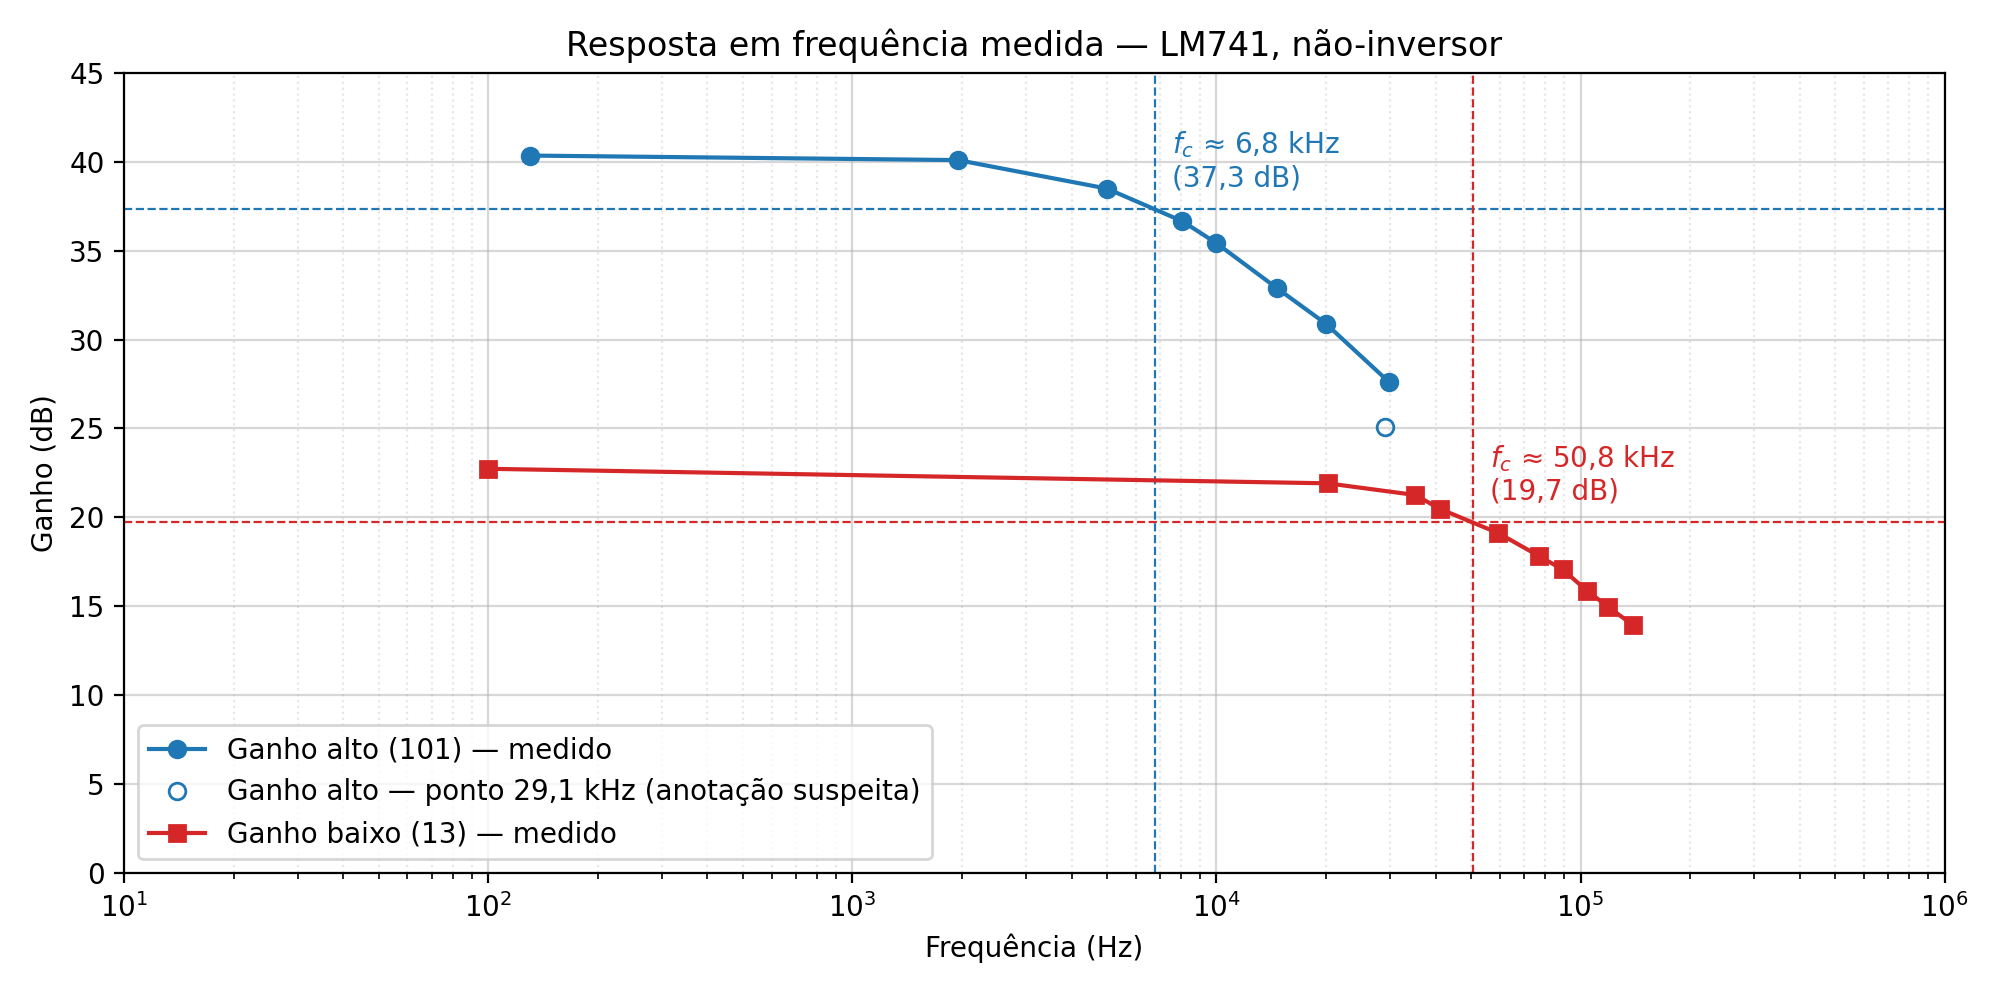
\includegraphics[width=\textwidth]{imgs/resultados/3.5_resposta_frequencia_medida.png}
\caption{Ganho medido em função da frequência para os estágios de ganho baixo (13) e ganho alto (101) com o LM741, com as frequências de corte lidas em $0{,}707$ do ganho de referência.}
\label{fig:resposta_freq_medida}
\end{figure}

\begin{figure}[H]
\centering
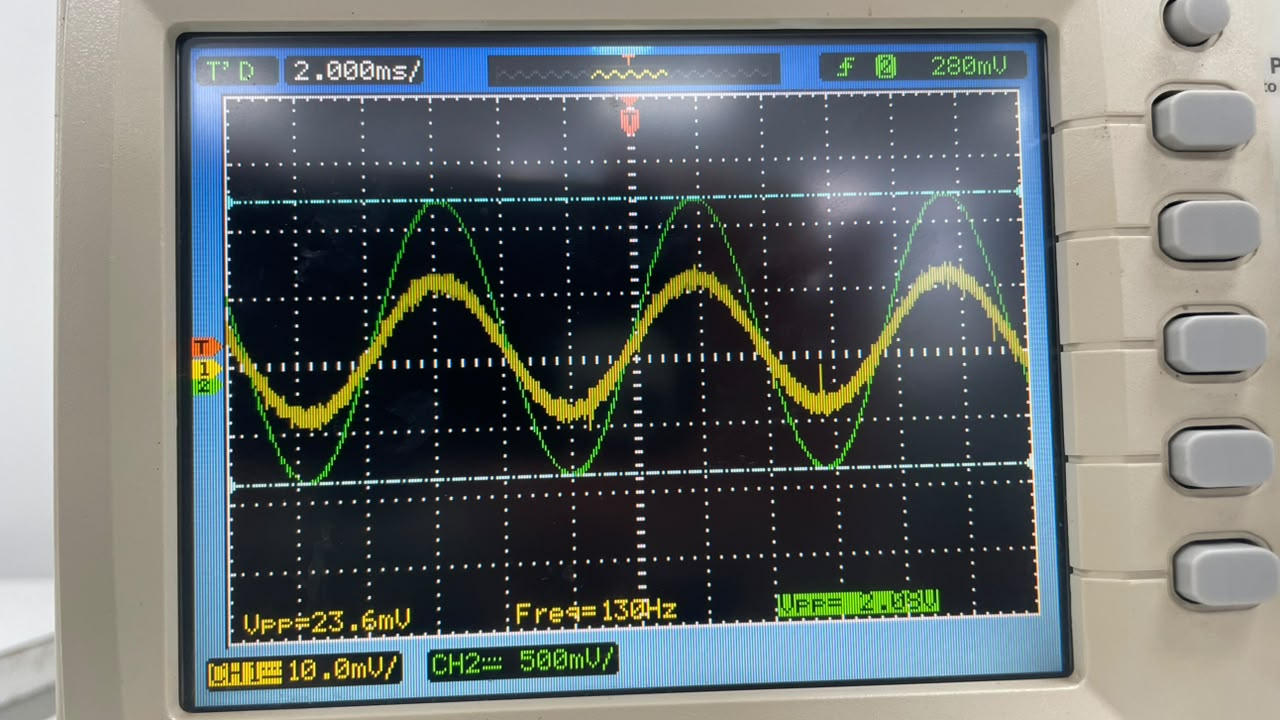
\includegraphics[width=0.75\textwidth]{imgs/resultados/3.5Ganho_alto_ruído_de_alta_frequencia.jpeg}
\caption{Estágio de ganho 101 em 130~Hz: entrada no CH1 (10~mV/div, $23{,}6$~mV pico a pico, com ruído de alta frequência sobreposto) e saída no CH2 (500~mV/div, $2{,}08$~V pico a pico).}
\label{fig:ganho_alto_ruido}
\end{figure}

Com o \textit{slew rate} típico do LM741 ($0{,}5$~V/$\mu$s), uma senoide de 1~V de pico passa a ser limitada a partir de $f=SR/(2\pi\cdot1~\mathrm{V})\approx79{,}6$~kHz, ou $\approx75{,}4$~kHz para os $\approx1{,}05$~V de pico ($2{,}11$~V pico a pico) usados no ganho baixo. O corte medido do ganho baixo, $50{,}8$~kHz, fica abaixo desse limite.

\subsubsection{Slew rate}

Com o amplificador em seguidor de tensão e senoide de $V_p=2{,}5$~V ($5{,}00$~V pico a pico na entrada do TL064, conforme a Figura~\ref{fig:slew_tl064_medido}), a frequência foi aumentada a partir de 1~kHz até a saída se tornar triangular. As capturas das Figuras~\ref{fig:slew_lm741_medido} e~\ref{fig:slew_tl064_medido} foram feitas em $56{,}8$~kHz no LM741 e em $52{,}6$~kHz no TL064.

Os cursores do osciloscópio estavam no modo amplitude, que fornece apenas $\Delta V$ entre o vale e o pico da rampa. O intervalo da rampa foi tomado como meio período do sinal, medido pelo frequencímetro, supondo triângulo simétrico:
\[
SR=\frac{\Delta V}{T/2}=2f\,\Delta V.
\]
A frequência a partir da qual uma senoide de amplitude $V_p$ passa a ser limitada é $f_{SR}=SR/(2\pi V_p)$. Os resultados estão na Tabela~\ref{tab:slew_equipe}.

\begin{table}[H]
\centering
\caption{\textit{Slew rate} medido no seguidor de tensão, com $V_p=2{,}5$~V.}
\label{tab:slew_equipe}
\renewcommand{\arraystretch}{1.2}
\begin{tabular}{@{}lcc@{}}
\toprule
\textbf{Grandeza} & \textbf{LM741} & \textbf{TL064} \\
\midrule
Frequência da captura (triângulo) & $56{,}8$~kHz & $52{,}6$~kHz \\
$\Delta V$ nos cursores & $4{,}52$~V & $4{,}60$~V \\
$\Delta t=T/2$ & $8{,}80~\mu$s & $9{,}51~\mu$s \\
\textit{Slew rate} medido & $0{,}51$~V/$\mu$s & $0{,}48$~V/$\mu$s \\
\textit{Slew rate} do datasheet (típ.) & $0{,}5$~V/$\mu$s & $3{,}5$~V/$\mu$s \\
$f_{SR}$ com o SR do datasheet & $31{,}8$~kHz & $223$~kHz \\
$f_{SR}$ com o SR medido & $32{,}7$~kHz & $30{,}8$~kHz \\
\bottomrule
\end{tabular}
\end{table}

Pela retícula das fotos (5~$\mu$s/div), as rampas não são exatamente simétricas: no LM741, a subida leva $\approx8{,}2~\mu$s ($\approx0{,}55$~V/$\mu$s) e a descida $\approx9{,}4~\mu$s ($\approx0{,}48$~V/$\mu$s); no TL064, a subida leva $\approx8{,}9~\mu$s ($\approx0{,}52$~V/$\mu$s) e a descida $\approx9{,}8~\mu$s ($\approx0{,}47$~V/$\mu$s). Na captura do TL064, o cursor foi lido na escala do CH1 (1,00~V/div), enquanto a saída está no CH2 (980~mV/div), diferença de 2\%. Na captura do LM741, os dois canais aparecem triangulares e sobrepostos. A razão entre os \textit{slew rates} medidos é $SR_{\mathrm{TL064}}/SR_{\mathrm{LM741}}\approx0{,}94$, enquanto a razão entre os valores típicos dos datasheets é $3{,}5/0{,}5=7$.

\begin{figure}[H]
\centering
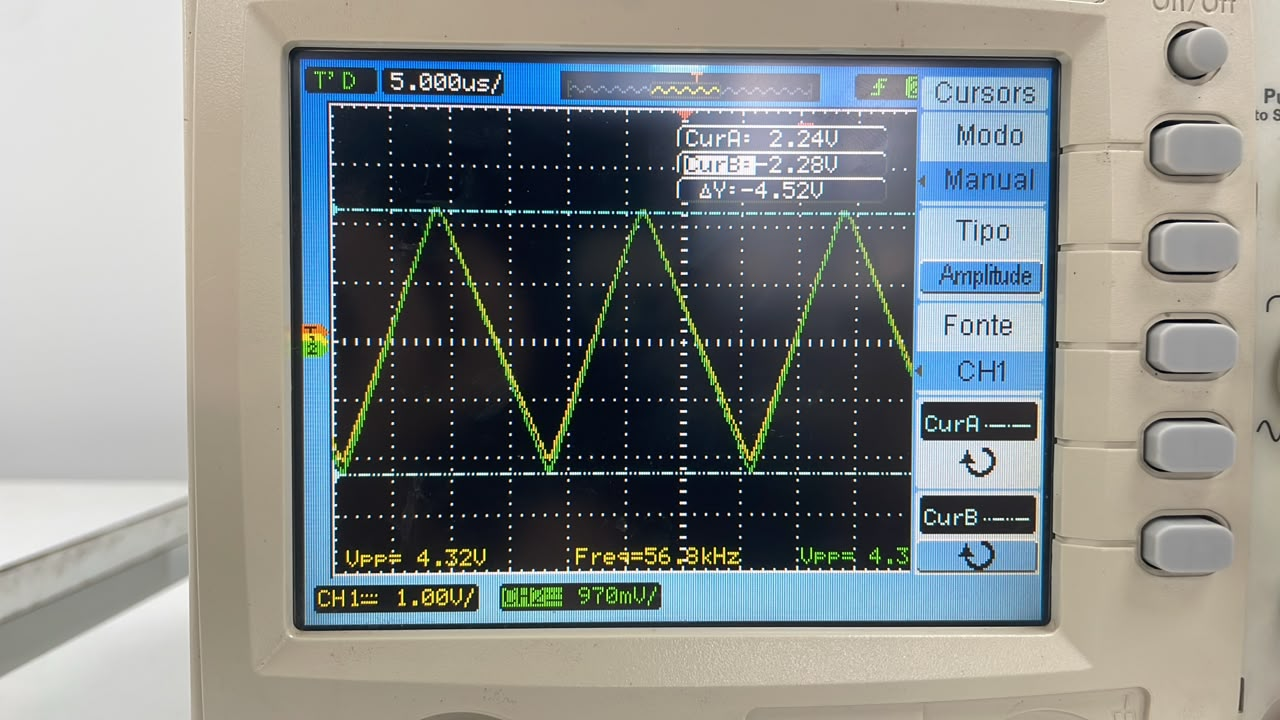
\includegraphics[width=0.75\textwidth]{imgs/resultados/3.6_Slew_rate_LM741.jpeg}
\caption{Seguidor de tensão com o LM741 em $56{,}8$~kHz: saída triangular, com $\Delta V=4{,}52$~V entre os cursores.}
\label{fig:slew_lm741_medido}
\end{figure}

\begin{figure}[H]
\centering
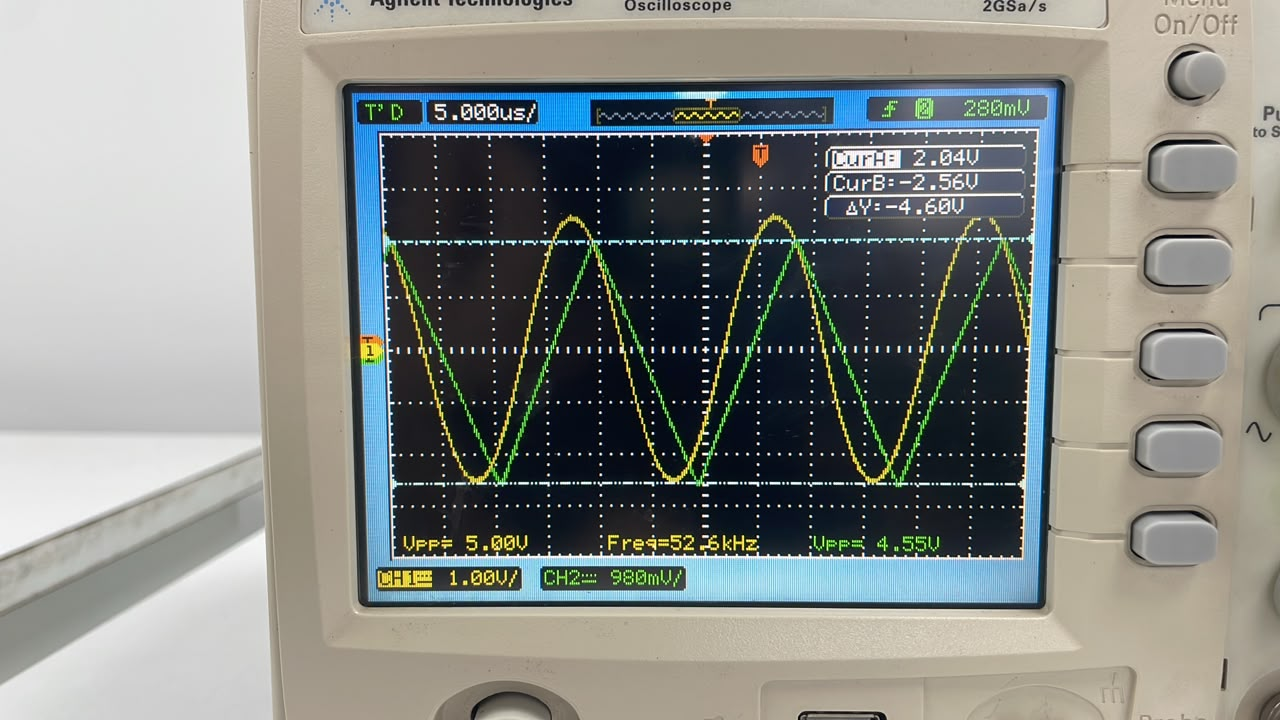
\includegraphics[width=0.75\textwidth]{imgs/resultados/3.6_Slew_rate_TL064.jpeg}
\caption{Seguidor de tensão com o TL064 em $52{,}6$~kHz: entrada senoidal no CH1 ($5{,}00$~V pico a pico) e saída triangular no CH2 ($4{,}55$~V pico a pico), com $\Delta V=4{,}60$~V entre os cursores.}
\label{fig:slew_tl064_medido}
\end{figure}

\subsubsection{Quadro-resumo}

A Tabela~\ref{tab:resumo_equipe} confronta, para cada grandeza, o valor de projeto (cálculo com os resistores nominais ou valor do datasheet), o resultado da simulação da montagem (Seção~4.3, com os valores medidos dos resistores) e o valor medido. O erro é calculado em relação à simulação da montagem; quando não há valor simulado, em relação ao projeto (marcado com $^{\dagger}$). Para a tensão de offset e a corrente de polarização do TL064, o erro não é apresentado: o datasheet fornece apenas uma faixa, e o modelo simulado do TL064 não apresenta corrente de entrada mensurável ($I(R_s)\sim10^{-23}$~A, com $\Delta V_O=-72~\mu$V).

\begin{table}[H]
\centering
\caption{Projeto, simulação da montagem e medição da Equipe 2.}
\label{tab:resumo_equipe}
\renewcommand{\arraystretch}{1.2}
\begin{tabular}{@{}lrrrr@{}}
\toprule
\textbf{Grandeza} & \textbf{Projeto} & \textbf{Sim. montagem} & \textbf{Medido} & \textbf{Erro} \\
\midrule
$V_{OS}$, LM741 & típ. $1$~mV & $1{,}13$~mV & $1{,}67$~mV & $+48\%$ \\
$V_{OS}$, TL064 & típ. $3$~mV & $0{,}027$~mV & $-0{,}490$~mV & -- \\
$I_B$, LM741 & típ. $80$~nA & $-59{,}4$~nA & $-16{,}7$~nA & $-72\%$ \\
$I_B$, TL064 & típ. $30$~pA & $\approx0$ & $+8{,}23$~nA & -- \\
Ganho baixo $G_1$ & $13{,}20$ & $13{,}16$ & $13{,}70$ & $+4{,}1\%$ \\
Ganho alto $G_2$ & $101{,}0$ & $103{,}7$ & $104{,}0$ & $+0{,}2\%$ \\
Corte $f_{c1}$ (ganho baixo) & -- & $95{,}0$~kHz & $50{,}8$~kHz & $-47\%$ \\
Corte $f_{c2}$ (ganho alto) & -- & $10{,}0$~kHz & $6{,}83$~kHz & $-32\%$ \\
$GBW_1$ (ganho baixo) & -- & $1{,}25$~MHz & $0{,}70$~MHz & $-44\%$ \\
$GBW_2$ (ganho alto) & -- & $1{,}04$~MHz & $0{,}71$~MHz & $-32\%$ \\
\textit{Slew rate}, LM741 & $0{,}5$~V/$\mu$s & -- & $0{,}51$~V/$\mu$s & $+3\%^{\dagger}$ \\
\textit{Slew rate}, TL064 & $3{,}5$~V/$\mu$s & -- & $0{,}48$~V/$\mu$s & $-86\%^{\dagger}$ \\
$f_{SR}$ ($V_p=2{,}5$~V), LM741 & $31{,}8$~kHz & -- & $32{,}7$~kHz & $+3\%^{\dagger}$ \\
$f_{SR}$ ($V_p=2{,}5$~V), TL064 & $223$~kHz & -- & $30{,}8$~kHz & $-86\%^{\dagger}$ \\
\bottomrule
\end{tabular}
\end{table}

\section{Discussão}

A discussão segue as três comparações do quadro da Seção~4: a conta contra a simulação de projeto,
esta contra a simulação da montagem, e esta contra a medição. Cada passo isola uma causa
diferente.

\subsection{Cálculo analítico contra simulação de projeto}

\paragraph{Ganhos.} Os ganhos simulados reproduzem a Equação~\eqref{eq:ganho_ni} com erro abaixo
de $0{,}1\%$ nos projetos de Guilherme ($0{,}03\%$ e $0{,}05\%$) e de Daniel ($0{,}06\%$ e
$0{,}10\%$). Na simulação de Lurian, os patamares de $28$ e $41{,}5$~dB coincidem com
$20\log 25=27{,}96$~dB e $20\log 119=41{,}51$~dB dentro da resolução da leitura gráfica. O pequeno
resíduo é sempre negativo e cresce com o ganho, como prevê o ganho de malha aberta finito:
$G_{\text{real}}\approx G\,(1-G/A_0)$, que, com $A_0\approx2\times10^5$ (200~V/mV, típico do
LM741), reduz o ganho 101 em $0{,}05\%$, exatamente o desvio simulado por Guilherme. A álgebra e os
esquemáticos estão, portanto, corretos.

\paragraph{Produto ganho-banda.} Nas seis curvas de resposta em frequência, o produto $G\cdot f_c$
ficou entre $0{,}99$ e $1{,}0$~MHz: $993$ e $991$~kHz para Guilherme, $996$ e $999$~kHz para Daniel
e cerca de $1$~MHz, por leitura gráfica, para Lurian. A Equação~\eqref{eq:fc_gbw} se confirma no
modelo, que se comporta como um polo dominante com $GBW\approx1$~MHz.

\paragraph{Comparação entre os integrantes.} Como os ganhos vieram de matrículas diferentes, as
frequências de corte também diferem, e a diferença é a que a Equação~\eqref{eq:fc_gbw} prevê.
Entre o menor ganho ($G_1=25$, Lurian) e o maior ($G_2=119$, Lurian), o corte caiu de cerca de
$40$ para cerca de $8$~kHz, razão de $5$, próxima da razão entre os ganhos, $119/25=4{,}8$. Entre
os ganhos intermediários, $G=35$ e $37$ deram $28{,}5$ e $27{,}0$~kHz, e $G=101$ e $116$ deram
$9{,}82$ e $8{,}62$~kHz, novamente na proporção inversa dos ganhos. No \textit{slew rate}, o valor
simulado do LM741 foi o mesmo nos três projetos ($0{,}315$ a $0{,}32$~V/$\mu$s), embora as
amplitudes fossem $5$~V (Guilherme) e $4{,}5$~V (Daniel e Lurian). Isso confirma que o
\textit{slew rate} é uma propriedade da peça e não do sinal. O que muda com a amplitude é a
fronteira da Equação~\eqref{eq:fsr}: $10{,}0$~kHz com $5$~V e $11{,}3$~kHz com $4{,}5$~V, razão
$1{,}11$, igual a $5/4{,}5$. Os ensaios de corrente contínua não variam entre os integrantes,
porque o ganho 101 e o resistor $R_s=100$~k$\Omega$ são fixados pelo roteiro.

\paragraph{Grandezas do componente.} Para offset, corrente de polarização e \textit{slew rate}
não existe cálculo analítico, e a comparação é entre o modelo e o valor típico do
\textit{datasheet}. O modelo do LM741 tem $V_{OS}=1{,}10$~mV (típico $1$~mV) e $I_B=57{,}8$~nA
(típico $80$~nA), ambos plausíveis. O \textit{slew rate} do modelo, $\approx0{,}32$~V/$\mu$s, está
cerca de $36\%$ abaixo do típico de $0{,}5$~V/$\mu$s. No TL064, o modelo tem $SR\approx3{,}2$ a
$3{,}3$~V/$\mu$s, $6$ a $9\%$ abaixo do típico de $3{,}5$~V/$\mu$s da Tabela~\ref{tab:datasheet_equipe}
(as tabelas da Seção~5.1 usaram $3{,}0$~V/$\mu$s como referência), e corrente de polarização nula
para fins práticos. No modelo, o TL064 é cerca de dez vezes mais rápido que o LM741, contra sete
vezes pelos valores típicos. Essas diferenças dizem o que o modelo representa, e não indicam erro
de projeto.

\subsection{Simulação de projeto contra simulação da montagem}

Os resistores medidos (Tabela~\ref{tab:resistores_bancada}) se afastam no máximo $1{,}8\%$ dos
nominais. O efeito sobre o ganho depende de como os desvios se combinam. No ganho alto, $R_f$ ficou
$1{,}0\%$ acima e $R_g$ ficou $1{,}7\%$ abaixo, e os dois desvios somam: o ganho passou de $101$
para $103{,}75$ ($+2{,}7\%$). No ganho baixo, $R_f'$ e $R_g'$ ficaram ambos cerca de $1{,}7\%$
abaixo, os desvios quase se cancelam na razão, e o ganho passou de $13{,}20$ para $13{,}16$
($-0{,}2\%$).

\paragraph{Offset e corrente de polarização.} A saída simulada do LM741 subiu de $111{,}13$~mV
(projeto) para $113{,}98$~mV (montagem), aumento de $2{,}6\%$, praticamente igual ao aumento do
ganho. Dividindo pelo ganho real, o offset do modelo é $0{,}113975/103{,}75=1{,}10$~mV, o mesmo da
simulação de projeto. O valor de $1{,}13$~mV da Seção~4.3 resulta apenas de dividir pelo ganho
nominal. O mesmo vale para a corrente de polarização: com o ganho real e $R_s=98{,}77$~k$\Omega$,
$I_B=0{,}592477/(103{,}75\cdot98{,}77~\text{k}\Omega)=57{,}8$~nA, idêntico aos $57{,}8$~nA do
projeto. A tolerância muda as leituras de saída em alguns por cento, mas não muda o parâmetro
extraído, desde que se use o ganho real. Por isso, a Equação~\eqref{eq:ib} foi aplicada à bancada
também com o ganho medido, o que dá $V_{OS}=169/103{,}75=1{,}63$~mV e
$I_B=-166{,}3~\text{mV}/(103{,}75\cdot98{,}77~\text{k}\Omega)=-16{,}2$~nA para o LM741, e
$V_{OS}=-0{,}477$~mV e $I_B=+8{,}0$~nA para o TL064. Esses valores diferem em cerca de $3\%$ dos
apresentados na Tabela~\ref{tab:offset_ib_equipe}, calculados com o ganho nominal de 101.

\paragraph{Resposta em frequência.} No ganho alto, a montagem simulada deu $f_{c2}=10{,}0$~kHz e
$GBW_2=1{,}04$~MHz, $4\%$ acima do $\approx1{,}0$~MHz do projeto, diferença compatível com a leitura
gráfica do corte. No ganho baixo, porém, $f_{c1}=95{,}0$~kHz dá $GBW_1=1{,}25$~MHz, $25\%$ acima.
Essa diferença não vem da tolerância: o ganho mudou só $0{,}2\%$, e com $GBW=1{,}0$~MHz o corte
esperado seria $1{,}0~\text{MHz}/13{,}16\approx76$~kHz. Na Figura~\ref{fig:sim_gbw}, as duas curvas
seguem a mesma assíntota acima de cerca de 200~kHz e cruzam $0$~dB no mesmo ponto, perto de 1~MHz,
o que indica um único $GBW$ para os dois estágios. O valor de $95$~kHz deve, portanto, vir da
leitura do joelho da curva de ganho baixo, que é suave e foi lida sem cursor. Uma medida com
\texttt{.meas} no ponto de $-3$~dB resolveria a dúvida.

\paragraph{\textit{Slew rate}.} O seguidor de tensão não tem resistores, e a simulação da montagem
é igual à de projeto. As simulações da Seção~4.3 no LM741 foram feitas entre 10~Hz e 1~kHz, abaixo
do limite de $\approx20$~kHz calculado com o \textit{slew rate} do modelo, e mostram a saída
acompanhando a senoide. Elas confirmam o regime linear, mas não medem o \textit{slew rate}. Para a
comparação com a bancada usa-se o valor das simulações de projeto, $\approx0{,}32$~V/$\mu$s.

\subsection{Simulação da montagem contra medição}

\paragraph{Ganho.} O ganho alto medido em baixa frequência, $104{,}0$, está a $0{,}2\%$ do valor
calculado com os resistores medidos ($103{,}75$). Esse acordo era esperado, porque em baixa
frequência o ganho depende só da razão entre os resistores (Equação~\eqref{eq:ganho_ni}). Ele
confirma a montagem e a leitura do osciloscópio, mas não diz nada sobre o amplificador, que nessa
condição se comporta como ideal. Comparado ao ganho nominal de 101, o mesmo resultado mostraria um
erro de $3\%$ que não existe: é a tolerância dos resistores, e não o circuito. No ganho baixo, o
valor medido de $13{,}70$ está $4{,}1\%$ acima de $13{,}16$. Na Tabela~\ref{tab:freq_g1_equipe}, a
razão $V_o/V_i$ fica em torno de $13{,}7$ em todas as frequências, enquanto $V_i$ cai junto com
$V_o$. Um sinal de entrada que acompanha a saída dessa forma é o que se veria com o canal de
entrada na entrada inversora, onde $V_-=V_o\,R_g'/(R_f'+R_g')$, em vez de na saída do gerador. Nessa
hipótese, $V_o/V_i$ é a razão do divisor de realimentação, e os $4\%$ restantes ficam por conta da
exatidão de ganho vertical dos dois canais do osciloscópio, especificada em $\pm3\%$ por canal.
Para evitar a dúvida, o canal de entrada deveria ficar no terminal do gerador durante toda a
varredura.

\paragraph{Produto ganho-banda.} Os dois produtos medidos, $0{,}70$ e $0{,}71$~MHz, coincidem
dentro de $2\%$, apesar de os ganhos diferirem por um fator de oito. Na assíntota do ganho alto,
$G\cdot f$ também fica entre $0{,}70$ e $0{,}72$~MHz. O modelo de polo dominante vale para a peça
real. O valor absoluto, porém, está cerca de $30\%$ abaixo dos $1{,}04$~MHz da simulação da
montagem ($f_{c2}=6{,}83$~kHz contra $10{,}0$~kHz). A tolerância dos resistores não explica a
diferença, porque o ganho medido coincide com o simulado. A instrumentação também não: o
osciloscópio tem banda de 60~MHz, e a ponta de prova está ligada à saída do amplificador, um nó de
baixa impedância. A causa é a própria peça. O \textit{datasheet} do LM741 não especifica banda nem
produto ganho-banda, e o modelo usa um valor típico de cerca de 1~MHz, enquanto a unidade usada na
bancada tem $\approx0{,}7$~MHz. Também foi verificado que o corte medido é de banda, e não de
\textit{slew rate}: com o \textit{slew rate} medido de $0{,}51$~V/$\mu$s e saída de
$\approx1{,}05$~V de pico, a distorção só começaria em $0{,}51/(2\pi\cdot1{,}05)\approx77$~kHz,
acima do corte de $50{,}8$~kHz. Foi para garantir essa folga que a amplitude de saída foi mantida
baixa, e menor ainda no ganho baixo, cujo corte é o mais alto.

\paragraph{Offset.} Os offsets medidos, $1{,}63$~mV no LM741 e $-0{,}48$~mV no TL064, diferem dos
do modelo ($1{,}10$ e $0{,}027$~mV), mas ambos estão dentro do máximo do \textit{datasheet}
($5$ e $15$~mV). O offset vem do descasamento aleatório entre os transistores do par diferencial, e
cada unidade tem o seu, com qualquer sinal. O modelo descreve uma unidade típica, e por isso essa
diferença não indica falha do modelo. Com uma única unidade de cada CI, o ensaio permite afirmar que
as peças estão dentro da especificação, mas não estimar a dispersão do componente.

\paragraph{Corrente de polarização no LM741.} A saída desceu quando $R_s$ entrou, o que indica
corrente entrando no pino não inversor, como previsto na Seção~2 para a corrente de base de um par
de entrada NPN. O módulo medido, $16{,}2$~nA, é cerca de $3{,}5$ vezes menor que os $57{,}8$~nA do
modelo e está abaixo do típico de $80$~nA. A corrente de base é inversamente proporcional ao ganho
de corrente $\beta$ dos transistores de entrada, que varia bastante entre unidades. Uma unidade
com $\beta$ alto explica o valor, que está dentro da especificação (máximo de $500$~nA).

\paragraph{Corrente de polarização no TL064.} O valor medido, $+8{,}0$~nA, é cerca de $20$ vezes
o máximo do \textit{datasheet} ($400$~pA a $25\,^\circ$C) e $270$ vezes o típico. Na entrada JFET,
a corrente é apenas a fuga reversa da junção porta-canal, e o modelo a dá como nula. O valor
medido, portanto, não é a corrente da peça. A causa mais provável é uma fuga no protoboard: uma
resistência de $15~\text{V}/8~\text{nA}\approx1{,}9$~G$\Omega$ entre o trilho de $+15$~V e o nó de
$100$~k$\Omega$ bastaria para produzir o degrau, e ela injetaria corrente no nó, elevando a saída,
que é exatamente o sentido observado. Outras causas possíveis são a deriva do offset entre as duas
leituras (bastariam $0{,}8$~mV na entrada) e a captação de rede no nó de alta impedância. Mesmo sem
nenhuma dessas causas, o arranjo não teria resolução para medir o TL064: $30$~pA em
$R_s\approx100$~k$\Omega$ produzem na saída apenas
$30~\text{pA}\cdot98{,}77~\text{k}\Omega\cdot103{,}75\approx0{,}3$~mV, da ordem da deriva entre
leituras. Para medir a corrente real seriam necessários um resistor de teste da ordem de
G$\Omega$, um capacitor em paralelo com $R_s$ para filtrar a captação e leituras alternadas com e
sem $R_s$. O resultado do TL064 deve ser lido como um limite superior.

\paragraph{\textit{Slew rate} no LM741.} O valor medido, $0{,}51$~V/$\mu$s, está a $3\%$ do típico
do \textit{datasheet} e $60\%$ acima dos $0{,}32$~V/$\mu$s do modelo. O modelo subestima o
\textit{slew rate} desta unidade, enquanto o \textit{datasheet} o descreve bem. A coincidência com o
típico era esperada para uma peça comum, mas, sendo uma única unidade, não permite estimar a
dispersão do lote. A incerteza da medida é de cerca de $\pm8\%$, porque o intervalo da rampa foi
tomado como meio período, e as rampas de subida e de descida diferem ($0{,}55$ e $0{,}48$~V/$\mu$s).
Essa assimetria é característica do estágio de saída do LM741. Medir a rampa com os cursores de
tempo eliminaria a suposição de triângulo simétrico.

\paragraph{\textit{Slew rate} no TL064.} O valor medido, $0{,}48$~V/$\mu$s, está $86\%$ abaixo do
típico de $3{,}5$~V/$\mu$s, abaixo do mínimo de $1{,}5$~V/$\mu$s a $25\,^\circ$C, e cerca de sete
vezes abaixo do modelo. Ele é, além disso, praticamente igual ao do LM741 (razão $0{,}94$). Uma
peça dentro da especificação não produziria esse valor. A coincidência com o LM741 sugere que, no
ensaio do seguidor, o sinal ainda passava pelo LM741, ou que a realimentação não foi refeita na
pinagem de 14 terminais do TL064, que é diferente da pinagem de 8 terminais do LM741. O ensaio
precisaria ser repetido com a pinagem conferida. Até lá, a bancada não confirma que o TL064 seja
mais rápido que o LM741, o que as simulações (fator $\approx10$) e o \textit{datasheet} (fator 7)
preveem.

\subsection{Retomada das hipóteses}

A hipótese de operação linear na região ativa se confirmou nos ensaios de corrente contínua e de
resposta em frequência: todas as saídas ficaram longe dos trilhos de alimentação, e a folga até o
limite de \textit{slew rate} foi verificada. O ganho ideal da Equação~\eqref{eq:ganho_ni} vale em
baixa frequência dentro de $0{,}2\%$, desde que se usem os valores medidos dos resistores. O modelo
de polo dominante (Equação~\eqref{eq:fc_gbw}) se confirmou na bancada, com o mesmo produto
ganho-banda nos dois ganhos, embora o valor da peça seja $30\%$ menor que o do modelo. As
Equações~\eqref{eq:vos} e~\eqref{eq:ib} descreveram o LM741 em sinal e ordem de grandeza. A
fronteira da Equação~\eqref{eq:fsr} é compatível com o LM741: a saída era senoidal em 1~kHz e
triangular em $56{,}8$~kHz, acima dos $32{,}7$~kHz previstos, embora a frequência exata de início da
distorção não tenha sido registrada. A única contradição entre previsão e medida, a do TL064 em
corrente de polarização e \textit{slew rate}, foi atribuída acima à montagem e não ao modelo.

\section{Conclusão}

O objetivo era medir as não idealidades de dois amplificadores operacionais, situá-las nas faixas
do \textit{datasheet} e separar experimentalmente a limitação linear de banda da limitação não
linear por \textit{slew rate}. Para o LM741, o objetivo foi atingido: offset de $1{,}63$~mV
(máximo de $5$~mV), corrente de polarização de $16$~nA entrando no pino (máximo de $500$~nA),
produto ganho-banda de $0{,}70$~MHz igual nos dois ganhos dentro de $2\%$, e \textit{slew rate}
de $0{,}51$~V/$\mu$s, a $3\%$ do típico. A separação entre os dois regimes também foi mostrada: o
corte de $50{,}8$~kHz do ganho baixo ficou abaixo do limite de \textit{slew rate} de $77$~kHz para
a amplitude usada, enquanto no seguidor com $2{,}5$~V de pico a distorção aparece a partir de
$\approx33$~kHz.

As simulações dos três integrantes confirmaram $f_c=GBW/G$ com $GBW\approx1$~MHz para ganhos de
25 a 119, e mostraram que a tolerância dos resistores muda as leituras de saída sem mudar os
parâmetros extraídos, desde que se use o ganho real. Na bancada, a peça real teve produto
ganho-banda $30\%$ menor e \textit{slew rate} $60\%$ maior que o modelo.

A principal limitação está nos ensaios do TL064. Seu offset está dentro da especificação, mas a
corrente de polarização ($8$~nA, contra o máximo de $400$~pA) e o \textit{slew rate}
($0{,}48$~V/$\mu$s, contra o mínimo de $1{,}5$~V/$\mu$s) não correspondem à peça. Por isso, o
relatório não pode afirmar, com base na bancada, qual é a corrente de polarização do TL064 nem
quantas vezes ele é mais rápido que o LM741. Além disso, a incerteza instrumental das leituras não
foi registrada, e foi usada uma única unidade de cada CI, de modo que as diferenças em relação ao
modelo não podem ser generalizadas para o componente.

\section{Referências}

\begin{referencias}
\item SEDRA, A.~S.; SMITH, K.~C. \emph{Microeletrônica}. 5.~ed. São Paulo: Pearson Prentice Hall, 2007.
\item BOYLESTAD, R.~L.; NASHELSKY, L. \emph{Dispositivos Eletrônicos e Teoria de Circuitos}. 11.~ed. São Paulo: Pearson Education do Brasil, 2013.
\item TEXAS INSTRUMENTS. \emph{LM741 General-Purpose Operational Amplifier}. Datasheet.
\item TEXAS INSTRUMENTS. \emph{TL064 Low-Power JFET-Input Operational Amplifiers}. Datasheet.
\item AGILENT TECHNOLOGIES. \emph{33220A 20 MHz Function / Arbitrary Waveform Generator}. Manual do equipamento.
\item AGILENT TECHNOLOGIES. \emph{DSO1002A Digital Storage Oscilloscope}. Manual do equipamento.
\item ANALOG DEVICES. \emph{LTspice}. Documentação e guia de criação de símbolos.
\end{referencias}

\end{document}
